% Arquivo LaTeX de exemplo de dissertação/tese a ser apresentada à CPG do IME-USP
%
% Criação: Jesús P. Mena-Chalco
% Revisão: Fabio Kon e Paulo Feofiloff
% Adaptação para UTF8, biblatex e outras melhorias: Nelson Lago
%
% Except where otherwise indicated, these files are distributed under
% the MIT Licence. The example text, which includes the tutorial and
% examples as well as the explanatory comments in the source, are
% available under the Creative Commons Attribution International
% Licence, v4.0 (CC-BY 4.0) - https://creativecommons.org/licenses/by/4.0/


%%%%%%%%%%%%%%%%%%%%%%%%%%%%%%%%%%%%%%%%%%%%%%%%%%%%%%%%%%%%%%%%%%%%%%%%%%%%%%%%
%%%%%%%%%%%%%%%%%%%%%%%%%%%%%%% PREÂMBULO LaTeX %%%%%%%%%%%%%%%%%%%%%%%%%%%%%%%%
%%%%%%%%%%%%%%%%%%%%%%%%%%%%%%%%%%%%%%%%%%%%%%%%%%%%%%%%%%%%%%%%%%%%%%%%%%%%%%%%

% A opção twoside (frente-e-verso) significa que a aparência das páginas pares
% e ímpares pode ser diferente. Por exemplo, as margens podem ser diferentes ou
% os números de página podem aparecer à direita ou à esquerda alternadamente.
% Mas nada impede que você crie um documento "só frente" e, ao imprimir, faça
% a impressão frente-e-verso.
%
% Aqui também definimos a língua padrão do documento
% (a última da lista) e línguas adicionais.
%\documentclass[12pt,twoside,brazilian,english]{book}
\documentclass[12pt,twoside,english,brazilian]{book}

% Ao invés de definir o tamanho das margens, vamos definir os tamanhos do
% texto, do cabeçalho e do rodapé, e deixamos a package geometry calcular
% o tamanho das margens em função do tamanho do papel. Assim, obtemos o
% mesmo resultado impresso, mas com margens diferentes, se o tamanho do
% papel for diferente.
\usepackage[a4paper]{geometry}
\usepackage{csquotes}
\geometry{
  textwidth=152mm,
  hmarginratio=12:17, % 24:34 -> com papel A4, 24mm + 152mm + 34mm = 210mm
  textheight=237mm,
  vmarginratio=8:7, % 32:28 -> com papel A4, 32mm + 237mm + 28mm = 297mm
  headsep=11mm, % distância entre a base do cabeçalho e o texto
  headheight=21mm, % qualquer medida grande o suficiente, p.ex., top - headsep
  footskip=10mm,
  marginpar=20mm,
  marginparsep=5mm,
}

% Vários pacotes e opções de configuração genéricos; para personalizar o
% resultado, modifique estes arquivos.
%%%%%%%%%%%%%%%%%%%%%%%%%%%%%%%%%%%%%%%%%%%%%%%%%%%%%%%%%%%%%%%%%%%%%%%%%%%%%%%%
%%%%%%%%%%%%%%%%%%%%%%% CONFIGURAÇÕES E PACOTES BÁSICOS %%%%%%%%%%%%%%%%%%%%%%%%
%%%%%%%%%%%%%%%%%%%%%%%%%%%%%%%%%%%%%%%%%%%%%%%%%%%%%%%%%%%%%%%%%%%%%%%%%%%%%%%%

% Vários comandos auxiliares para o desenvolvimento de packages e classes;
% aqui, usamos em alguns comandos de formatação e condicionais.
\usepackage{etoolbox}
%\RequirePackage{pdftexcmds}
\usepackage{letltxmacro}
%\usepackage{ltxcmds}

% LaTeX 3
\usepackage{expl3}
\usepackage{xparse}

%\usepackage{filehook}

% Detecta se estamos usando pdftex, luatex, xetex etc.
\usepackage{iftex}

%\usepackage{xfp} % Floating-point calculations

\usepackage{regexpatch}

% O projeto LaTeX3 renomeou algumas macros em 2019-03-05 e removeu
% a compatibilidade com os nomes antigos em 2020-07-17 a partir de
% 2021-01-01 (veja o arquivo l3deprecation.dtx e o changelog em
% https://github.com/latex3/latex3/blob/main/l3kernel/CHANGELOG.md).
% Isso afetou a package regexpatch: versões antigas da package não
% funcionam com versões novas de LaTeX e vice-versa. Infelizmente,
% ubuntu 21.04 (hirsute) e debian 11 (bullseye) incluem essas versões
% incompatíveis e, portanto, a package regexpatch não funciona nesses
% ambientes. Talvez fosse possível contornar esse problema com a
% package latexrelease, mas isso afetaria muitos outros recursos.
% Ao invés disso, vamos restaurar manualmente a compatibilidade.
% TODO: remover isto após debian bullseye se tornar obsoleta,
%       provavelmente no final de 2024.
\makeatletter
\ExplSyntaxOn
\@ifpackagelater{regexpatch}{2021/03/21}
  {} % Se regexpatch é "nova", expl3 deve ser também; nada a fazer
  {
    % Talvez o correto seja 2021/01/01, mas na prática o resultado é o mesmo
    \@ifpackagelater{expl3}{2020/07/17}
      {
        % As versões são incompatíveis; vamos recuperar as macros preteridas
        \cs_gset:Npn \token_get_prefix_spec:N { \cs_prefix_spec:N }
        \cs_gset:Npn \token_get_arg_spec:N { \cs_argument_spec:N }
        \cs_gset:Npn \token_get_replacement_spec:N { \cs_replacement_spec:N }
      }
      {} % As duas packages são antigas e, portanto, compatíveis entre si
  }
\ExplSyntaxOff
\makeatother

% Algumas packages dependem de xpatch e tentam carregá-la, causando conflitos
% com regexpatch. Como regexpatch oferece todos os recursos de xpatch (ela
% é uma versão estendida de xpatch, mas ainda considerada experimental), vamos
% fazê-las acreditar que xpatch já foi carregada.
\makeatletter
\@ifpackagelater{regexpatch}{2020/10/06}
    {\expandafter\xdef\csname ver@xpatch.sty\endcsname{2020/03/25}}
    {\expandafter\xdef\csname ver@xpatch.sty\endcsname{2012/10/02}}
\makeatother

% Acrescenta a correção deste bug (contida na release 2018-11-28):
% https://github.com/latex3/latex2e/issues/94 . Se a correção não
% puder ser aplicada, temos uma versão de LaTeX que já a incorpora.
% Esse bug afeta apenas textos em duas colunas.
% TODO: remover após ubuntu 18.04 se tornar obsoleta (abril/2023)
\makeatletter
\patchcmd\@combinedblfloats{\box\@outputbox}{\unvbox\@outputbox}{}{}
\makeatother

% Arithmetic expressions in \set{length,counter} & \addto{length,counter};
% commands \widthof, \heightof, \depthof, \totalheightof, \settototalheight
\usepackage{calc}

% Algumas packages "padrão" da AMS, que são praticamente obrigatórias.
% Algumas delas devem ser carregadas antes de unicode-math ou das
% definições das fontes do documento. É preciso carregar amsthm após
% amsmath para o comando \qedhere funcionar dentro do ambiente align.
\usepackage{amssymb}
\usepackage{amsmath}
\usepackage{amsthm}

% "fontenc" é um parâmetro do NFSS (sistema de gestão de fontes do
% LaTeX; consulte "texdoc fntguide" e "texdoc fontenc"). O default
% é OT1, mas ele tem algumas limitações; a mais importante é que,
% com ele, palavras acentuadas não podem ser hifenizadas. Por
% conta disso, quase todos os documentos LaTeX utilizam o fontenc
% T1. A escolha do fontenc tem consequências para as fontes que
% podem ser usadas com NFSS; hoje em dia T1 tem mais opções de
% qualidade, então não se perde nada em usá-lo. A package fontspec
% (para gestão de fontes usando outro mecanismo, compatível apenas
% com lualatex e xelatex) carrega fontenc automaticamente, mas
% usando outra codificação ("TU" e não "T1"). Ainda assim, é útil
% carregar o fontenc T1 (antes de carregar fontspec!) para o caso
% de alguma fonte "antiga" ser utilizada no documento (embora isso
% não seja recomendado: lualatex e xelatex só são capazes de
% hifenizar palavras acentuadas com o fontenc TU).
\usepackage[T1]{fontenc}

\ifPDFTeX
  % O texto está escrito em utf8.
  \usepackage[utf8]{inputenc}

  % Várias packages que definem as fontes do documento carregam fontaxes,
  % mas carregamos aqui porque, com qualquer fonte, ela permite utilizar
  % small caps + itálico. Algumas raras packages de fontes podem causar
  % conflitos com fontaxes, em geral por utilizarem a package "concorrente"
  % nfssext-cfr.
  %
  % TODO A funcionalidade pela qual faz sentido carregar fontaxes aqui
  %      (small caps + itálico) foi incorporada ao kernel do LaTeX na
  %      versão 2020-02-02, então está em TeXLive 2021. Remover isto
  %      quando arxiv usar TeXLive >= 2021 e ubuntu 20.04 (focal) for
  %      descontinuada (abril de 2025). As packages que precisam de
  %      fontaxes podem continuar a carregá-la sem problemas.
  \usepackage{fontaxes}

  % LaTeX substitui algumas sequências de caracteres, como
  % "fi", "fl" e outras, por caracteres especiais ("ligaduras").
  % Para que seja possível fazer copiar/colar ou buscas por
  % textos contendo essas ligaduras, o arquivo PDF precisa
  % conter uma tabela indicando quais são elas. Com fontes
  % OTF (LuaLaTeX ou XeLaTeX) isso não costuma ser um problema,
  % mas com pdfLaTeX pode ser. Estes dois comandos (que só
  % existem no pdfLaTeX) incluem uma tabela genérica que
  % funciona para a maioria das fontes. Veja a seção 5 de
  % http://www.tug.org/TUGboat/Articles/tb29-1/tb91thanh-fonts.pdf
  % Note que alguns visualizadores de PDF tentam "adivinhar"
  % o conteúdo da tabela quando ela está incompleta ou não
  % existe, então copiar/colar e buscas podem funcionar em
  % alguns visualizadores e em outros não.
  %
  % TODO Isto foi incluído no kernel do LaTeX versão 2021-06-01,
  %      então está em TeXLive 2022. Remover isto quando arxiv
  %      usar TeXLive >= 2022 e ubuntu 22.04 (jammy) for
  %      descontinuada (abril de 2027).
  \input glyphtounicode.tex
  \pdfgentounicode=1
\else
  % Não é preciso carregar inputenc com LuaTeX e XeTeX, pois
  % com eles utf8 é obrigatório.
  \usepackage{fontspec}

  % Ao invés de usar o sistema tradicional de LaTeX para gerir
  % as fontes matemáticas, utiliza as extensões matemáticas do
  % formato otf definidas pela microsoft. Ao ativar esta package
  % o mecanismo tradicional não funciona mais! Há poucas fontes
  % com suporte a unicode-math.
  \usepackage{unicode-math}
\fi

% Acesso a símbolos adicionais, como \textrightarrow, \texteuro etc.,
% disponíveis na maioria das fontes através do fontenc TS1 ou mudando
% momentaneamente para computer modern/latin modern. Raramente útil
% com lualatex/xelatex, mas não causa problemas. Várias packages de
% fontes carregam textcomp, às vezes com opções específicas; assim,
% para evitar problemas, vamos carregá-la no final do preâmbulo para
% o caso de ela não ter sido carregada antes.
%
% TODO A funcionalidade oferecida por textcomp foi incorporada ao kernel
%      do LaTeX na versão 2020-02-02, então está em TeXLive 2021. Remover
%      isto quando arxiv usar TeXLive >= 2021 e ubuntu 20.04 (focal) for
%      descontinuada (abril de 2025). As packages que precisam de textcomp
%      podem continuar a carregá-la sem problemas.
\AtBeginDocument{\usepackage{textcomp}}

% TeXLive 2018 inclui a versão 2.7a da package microtype e a versão
% 1.07 de luatex. Essa combinação faz aparecer um bug:
% https://tex.stackexchange.com/a/476742
% Aqui, aplicamos a solução sugerida, que não tem "contra-indicações".
% TODO: remover após ubuntu 18.04 se tornar obsoleta (abril/2023)
\ifLuaTeX
  \usepackage{luatexbase}
\fi

% microajustes no tamanho das letras, espaçamento etc. para melhorar
% a qualidade visual do resultado.
\usepackage{microtype}

% Alguns "truques" (sujos?) para minimizar over/underfull boxes.
%
% Para fazer um texto justificado, é preciso modificar o tamanho dos espaços
% em cada linha para mais ou para menos em relação ao seu tamanho ideal. Para
% escolher as quebras de linha, TeX vai percorrendo o texto procurando lugares
% possíveis para quebrar as linhas considerando essa flexibilidade mas dentro
% de um certo limite mínimo/máximo. Nesse processo, ele associa a cada possível
% linha o valor *badness*, que é o nível de distorção do tamanho dos espaços
% daquela linha em relação ao ideal, e ignora opções que tenham badness muito
% grande (esse limite é dado por \tolerance). Depois de encontradas todas
% as possíveis quebras de linha e a badness de cada uma, TeX calcula as
% *penalties* das quebras encontradas, que são uma medida de quebras "ruins".
% Por exemplo, na configuração padrão, quebrar uma linha hifenizando uma
% palavra gera uma penalty de 50; já uma quebra que faça a última linha
% do parágrafo ficar sozinha na página seguinte gera uma penalty de 150.
% Finalmente, TeX calcula a "feiúra" de cada possível linha (demerits)
% com base na badness e nas penalties e escolhe a solução que minimiza os
% demerits totais do parágrafo. Os comandos \linebreak e \pagebreak funcionam
% simplesmente acrescentando uma penalty negativa ao lugar desejado para a
% quebra.
%
% Para cada fonte, o espaço entre palavras tem um tamanho ideal, um
% tamanho mínimo e um tamanho máximo (é possível obter os valores com
% \number\fontdimenX\font\relax, veja https://tex.stackexchange.com/q/88991 ).
% TeX nunca reduz um espaço para menos que o mínimo da fonte, mas pode
% aumentá-lo para mais que o máximo. Se os espaços de uma linha ficam
% com o tamanho ideal, a badness da linha é 0; se o tamanho é
% reduzido/aumentado 50% do mínimo/máximo, a badness da linha é 12; se
% o tamanho é reduzido/aumentado para o mínimo/máximo, a badness é 100,
% e assim por diante. O valor máximo possível para badness é 10.000, que
% significa "badness infinita". Como é feito o cálculo: se as medidas
% do espaço definidas pela fonte são "x plus y minus z" e o tamanho
% final do espaço é "x + k*y" ou "x - k*z", a badness é 100*(k^3). Com
% Libertinus corpo 12, os valores são "3pt plus 1.5pt minus .9996pt",
% Então se o espaço tiver sido aumentado para 3.75pt, o fator é 0.5 e
% a badness é 100*(.5^3) = 12.
%
% \tolerance indica a badness máxima que TeX aceita para uma linha; seu valor
% default é 200. Assim, aumentar para, digamos, 300 ou 400, permite que
% TeX escolha parágrafos com maior variação no espaçamento entre as palavras.
% No entanto, no cálculo de demerits, a badness e as penalties de cada linha
% são elevadas ao quadrado, então TeX geralmente prefere escolher outras
% opções no lugar de uma linha com espaçamento ruim. Por exemplo, órfãs/viúvas
% têm demerit de 22.500 e dois hífens seguidos têm demerit de 10.000; já uma
% linha com badness 400 tem demerit 160.000. Portanto, não é surpreendente que
% a maioria dos parágrafos tenha demerits abaixo de 40.000, quase todos abaixo
% de 100.000 e praticamente nenhum acima de 1.000.000. Isso significa que, para
% a grande maioria dos parágrafos, aumentar \tolerance não faz diferença: uma
% linha com badness 400 nunca será efetivamente escolhida se houver qualquer
% outra opção com badness menor. Também fica claro que não há muita diferença
% real entre definir \tolerance como 800 ou 9.999 (a não ser fazer TeX
% trabalhar mais desnecessariamente).
%
% O problema muda de figura se TeX não consegue encontrar uma solução. Isso
% pode acontecer em dois casos: (1) o parágrafo tem ao menos uma linha que não
% pode ser quebrada com badness < 10.000 ou (2) o parágrafo tem ao menos uma
% linha que não pode ser quebrada com badness < tolerance (mas essa badness é
% menor que 10.000).
%
% No primeiro caso, se houver várias possibilidades de linhas que não podem ser
% quebradas, TeX não vai ser capaz de compará-las e escolher a melhor: todas
% têm a badness máxima (10.000) e, portanto, a que gerar menos deméritos no
% restante do parágrafo será a escolhida. Na realidade, no entanto, essas
% linhas *não* são igualmente ruins entre si, o que pode levar TeX a fazer uma
% má escolha. Para evitar isso, TeX tenta novamente aplicando
% \emergencystretch, que "faz de conta" que o tamanho máximo ideal dos espaços
% da linha é maior que o definido na fonte. Isso reduz a badness de todas as
% linhas, o que soa parecido com aumentar \tolerance. Há três diferenças, no
% entanto: (1) essa mudança só afeta os parágrafos que falharam; (2) soluções
% que originalmente teriam badness = 10.000 (e, portanto, seriam vistas como
% equivalentes) podem ser avaliadas e comparadas entre si; e (3) como a badness
% de todas as linhas diminui, a possibilidade de outras linhas que
% originalmente tinham badness alta serem escolhidas aumenta. Esse último ponto
% significa que \emergencystretch pode fazer TeX escolher linhas mais
% espaçadas, fazendo o espaçamento do parágrafo inteiro aumentar e, portanto,
% tornando o resultado mais homogêneo mesmo com uma linha particularmente ruim.
%
% É esse último ponto que justifica o uso de \emergencystretch no segundo caso
% também: apenas aumentar a tolerância, nesse caso, poderia levar TeX a
% diagramar uma linha ruim em meio a um parágrafo bom, enquanto
% \emergencystretch pode fazer TeX aumentar o espaçamento de maneira geral no
% parágrafo, minimizando o contraste da linha problemática com as demais.
% Colocando a questão de outra maneira, aumentar \tolerance para lidar com
% esses parágrafos problemáticos pode fazê-los ter uma linha especialmente
% ruim, enquanto \emergencystretch pode dividir o erro entre várias linhas.
% Assim, definir \tolerance em torno de 800 parece razoável: no caso geral,
% não há diferença e, se um desses casos difíceis não pode ser resolvido com
% uma linha de badness até 800, \emergencystretch deve ser capaz de gerar um
% resultado igual ou melhor.
%
% Penalties & demerits: https://tex.stackexchange.com/a/51264
% Definições (fussy, sloppy etc.): https://tex.stackexchange.com/a/241355
% Mais definições (hfuzz, hbadness etc.): https://tex.stackexchange.com/a/50850
% Donald Arseneau defendendo o uso de \sloppy: https://groups.google.com/d/msg/comp.text.tex/Dhf0xxuQ66E/QTZ7aLYrdQUJ
% Artigo detalhado sobre \emergencystretch: https://www.tug.org/TUGboat/tb38-1/tb118wermuth.pdf
% Esse artigo me leva a crer que algo em torno de 1.5em é suficiente

\tolerance=800
\hyphenpenalty=100 % Default 50; se o texto é em 2 colunas, 50 é melhor
\setlength{\emergencystretch}{1.5em}

% Não gera warnings para Overfull menor que 1pt
\hfuzz=1pt
\vfuzz\hfuzz

% Não gera warnings para Underfull com badness < 1000
\hbadness=1000
\vbadness=1000

% Por padrão, o algoritmo LaTeX para textos não-justificados é (muito) ruim;
% este pacote implementa um algoritmo bem melhor
\usepackage[newcommands]{ragged2e}

% ragged2e funciona porque permite que LaTeX hifenize palavras em textos
% não-justificados quando necessário. No caso de textos centralizados,
% no entanto, isso em geral não é desejável. Assim, newcommands não é
% interessante para \centering e \begin{center}. newcommands também
% causa problemas com legendas se o float correspondente usa \centering
% (o que é muito comum). Assim, vamos voltar \centering e \begin{center}
% à definição padrão.
\let\centering\LaTeXcentering
\let\center\LaTeXcenter
\let\endcenter\endLaTeXcenter

% Com ragged2e e a opção "newcommands", textos curtos não-justificados
% podem gerar warnings sobre "underfull \hbox". Não há razão para pensar
% muito nesses warnings, então melhor desabilitá-los.
% https://tex.stackexchange.com/a/18019
\makeatletter
\gappto{\raggedright}{\hbadness=\@M}
\gappto{\RaggedRight}{\hbadness=\@M}
\gappto{\raggedleft}{\hbadness=\@M}
\gappto{\RaggedLeft}{\hbadness=\@M}
\gappto{\Centering}{\hbadness=\@M} % not \centering
\gappto{\flushleft}{\hbadness=\@M}
\gappto{\FlushLeft}{\hbadness=\@M}
\gappto{\flushright}{\hbadness=\@M}
\gappto{\FlushRight}{\hbadness=\@M}
\gappto{\Center}{\hbadness=\@M} % not \center
\makeatother

% Espaçamento entre linhas configurável (\singlespacing, \onehalfspacing etc.)
\usepackage{setspace}

% LaTeX às vezes coloca notas de rodapé logo após o final do texto da
% página ao invés de no final da página; este pacote evita isso e faz
% notas de rodapé funcionarem corretamente em títulos de seções.
% Esta package deve ser carregada depois de setspace.
\usepackage[stable,bottom]{footmisc}

% Se uma página está vazia, não imprime número de página ou cabeçalho
\usepackage{emptypage}

% hyperref deve preferencialmente ser carregada próximo ao final
% do preâmbulo mas, para o caso de alguma package forçar a sua
% carga antes de executarmos \usepackage explicitamente, vamos
% garantir que estas opções estejam ativas.
\PassOptionsToPackage{
  unicode=true,
  pdfencoding=unicode,
  plainpages=false,
  pdfpagelabels,
  bookmarksopen=true,
  breaklinks=true,
  %hyperfootnotes=false, % polui desnecessariamente com bordercolor
}{hyperref}

% Carrega nomes de cores disponíveis (podem ser usados com hyperref e listings)
\usepackage[hyperref,svgnames,x11names,table]{xcolor}

% LaTeX oferece 2 pares de comandos nativos para mudar textos para caixa
% alta ou baixa: \uppercase ou \lowercase (TeX "puro") e \MakeUppercase
% ou \MakeLowecase (LaTeX), mas esses comandos têm algumas limitações
% (https://tug.org/TUGboat/tb41-1/tb127wright-case.pdf ). Esta package
% define os comandos \MakeTextUppercase e \MakeTextLowercase que resolvem
% isso.
% TODO: quando TeXLive 2023 for a versão mais antiga de LaTeX a que
%       estivermos dando suporte, podemos eliminar a package textcase
%       e usar \MakeUppercase e \MakeLowercase diretamente. A partir
%       dessa versão, essas macros usam \text_[upper|lower]case:n de
%       expl3.
\usepackage{textcase}

% Em documentos frente-e-verso, LaTeX faz o final da página terminar sempre
% no mesmo lugar (exceto no final dos capítulos). Esse comportamento pode ser
% ativado explicitamente com o comando "\flushbottom". Mas se, por alguma
% razão, o volume de texto na página é "pequeno", essa página vai ter espaços
% verticais artificialmente grandes. Uma solução para esse problema é utilizar
% "\raggedbottom" (padrão em documentos que não são frente-e-verso): com essa
% opção, as páginas podem terminar em alturas ligeiramente diferentes. Outra
% opção é corrigir manualmente cada página problemática, por exemplo com o
% comando "\enlargethispage".
%\raggedbottom
\flushbottom

% Por padrão, LaTeX coloca uma espaço aumentado após sinais de pontuação;
% Isso não é tão bom quanto alguns TeX-eiros defendem :) .
% Esta opção desabilita isso e, consequentemente, evita problemas com
% "id est" (i.e.) e "exempli gratia" (e.g.)
\frenchspacing

% Mais recursos para trechos de texto "puro" (tabs, quebras de linha etc.
% não são modificados), além do ambiente "\begin{comment}".
\usepackage{verbatim}

% Durante o processamento, LaTeX procura por arquivos adicionais necessários
% (tanto componentes do próprio LaTeX, como packages e fontes, quanto partes
% do conteúdo em si, como imagens carregadas com \includegraphics ou arquivos
% solicitados com \input ou \include) no diretório de instalação e também
% no diretório atual (ou seja, o diretório do projeto). Assim, normalmente
% é preciso usar caminhos relativos para incluir arquivos de subdiretórios:
% "\input{diretorio/arquivo}". No entanto, há duas limitações:
%
% 1. É necessário dizer "\input{diretorio/arquivo}" mesmo quando o arquivo
%    que contém esse comando já está dentro do subdiretório.
%
% 2. Isso não deve ser usado para packages ("\usepackage{diretorio/package}"),
%    embora na prática funcione.
%
% Há três maneiras recomendadas de resolver esses problemas:
%
% 1. Acrescentando os diretórios desejados ao arquivo texmf.cnf
%
% 2. Acrescentando os diretórios desejados às variáveis de ambiente
%    TEXINPUTS e BSTINPUTS
%
% 3. Colocando os arquivos adicionais na árvore TEXMF (geralmente, no
%    diretório texmf dentro do diretório do usuário).
%
% Essas soluções, no entanto, não podem ser automatizadas por este modelo
% e são um tanto complicadas para usuários menos experientes. Veja mais a
% respeito na seção 5 de "texdoc kpathsea" e em
% https://www.overleaf.com/learn/latex/Articles/An_introduction_to_Kpathsea_and_how_TeX_engines_search_for_files .
%
% A package import pode solucionar o primeiro problema, mas exige o uso
% de outro comando no lugar de \input, então não a usamos aqui.
%\usepackage{import}
%
% Uma solução mais simples é acrescentar os diretórios desejados à macro
% \input@path, originalmente criada para resolver um problema relacionado
% à portabilidade. Seu uso não é normalmente recomendado por razões de
% desempenho, mas no nosso caso (em que adicionamos apenas um diretório
% com poucos arquivos e com máquinas modernas) isso não é um problema. Veja
% https://tex.stackexchange.com/questions/241828/define-path-for-packages-in-the-latex-file-analog-of-inputpath-or-graphicspa#comment705011_241832
\csappto{input@path}{{extras/}}

%%%%%%%%%%%%%%%%%%%%%%%%%%%%%%%%%%%%%%%%%%%%%%%%%%%%%%%%%%%%%%%%%%%%%%%%%%%%%%%%
%%%%%%%%%%%%%%%%%%%%%%%%%%%%%%%%%%% LÍNGUAS %%%%%%%%%%%%%%%%%%%%%%%%%%%%%%%%%%%%
%%%%%%%%%%%%%%%%%%%%%%%%%%%%%%%%%%%%%%%%%%%%%%%%%%%%%%%%%%%%%%%%%%%%%%%%%%%%%%%%

\makeatletter
\ExplSyntaxOn

% We need to have at least some variant of Portuguese and of English
% loaded to generate the abstract/resumo, palavras-chave/keywords etc.
% We will make sure that both languages are present in the class options
% list by adding them if needed. With this, these options become global
% and therefore are seen by all packages (among them, babel).
%
% babel traditionally uses "portuguese", "brazilian", "portuges", or
% "brazil" to support the Portuguese language, using .ldf files. babel
% is also in the process of implementing a new scheme, using .ini
% files, based on the concept of "locales" instead of "languages". This
% mechanism uses the names "portuguese-portugal", "portuguese-brazil",
% "portuguese-pt", "portuguese-br", "portuguese", "brazilian", "pt",
% "pt-PT", and "pt-BR" (i.e., neither "portuges" nor "brazil"). To avoid
% compatibility problems, let's stick with "brazilian" or "portuguese"
% by substituting portuges and brazil if necessary.

\NewDocumentCommand\@IMEportugueseAndEnglish{m}{

  % Make sure any instances of "portuges" and "brazil" are replaced
  % by "portuguese" e "brazilian"; other options are unchanged.
  \seq_gclear_new:N \l_tmpa_seq
  \seq_gclear_new:N \l_tmpb_seq
  \seq_gset_from_clist:Nc \l_tmpa_seq {#1}

  \seq_map_inline:Nn \l_tmpa_seq{
    \def\@tempa{##1}
    \ifstrequal{portuges}{##1}
      {
        \GenericInfo{sbc2019}{}{Substituting~language~portuges~->~portuguese}
        \def\@tempa{portuguese}
      }
      {}
    \ifstrequal{brazil}{##1}
      {
        \GenericInfo{}{Substituting~language~brazil~->~brazilian}
        \def\@tempa{brazilian}
      }
      {}
    \seq_gput_right:NV \l_tmpb_seq {\@tempa}
  }

  % Remove the leftmost duplicates (default is to remove the rightmost ones).
  % Necessary in case the user did "portuges,portuguese", "brazil,brazilian"
  % or some variation: When we substitute the language, we end up with the
  % exact same language twice, which may mess up the main language selection.
  \seq_greverse:N \l_tmpb_seq
  \seq_gremove_duplicates:N \l_tmpb_seq
  \seq_greverse:N \l_tmpb_seq

  % If the user failed to select some variation of English and Portuguese,
  % we add them here. We also remember which ones of portuguese/brazilian,
  % english/american/british etc. were selected.
  \exp_args:Nnx \regex_extract_all:nnNTF
    {\b(portuguese|brazilian)\b}
    {\seq_use:Nn \l_tmpb_seq {,}}
    \l_tmpa_tl
    {
      \tl_reverse:N \l_tmpa_tl
      \xdef\@IMEpt{\tl_head:N \l_tmpa_tl}
    }
    {
      \seq_gput_left:Nn \l_tmpb_seq {brazilian}
      \gdef\@IMEpt{brazilian}
    }

  \exp_args:Nnx \regex_extract_all:nnNTF
    {\b(english|american|USenglish|canadian|british|UKenglish|australian|newzealand)\b}
    {\seq_use:Nn \l_tmpb_seq {,}}
    \l_tmpa_tl
    {
      \tl_reverse:N \l_tmpa_tl
      \xdef\@IMEen{\tl_head:N \l_tmpa_tl}
    }
    {
      \seq_gput_left:Nn \l_tmpb_seq {english}
      \gdef\@IMEen{english}
    }

  \exp_args:Nc \xdef {#1} {\seq_use:Nn \l_tmpb_seq {,}}
}


% https://tex.stackexchange.com/a/43541
% This message is part of a larger thread that discusses some
% limitations of this method, but it is enough for us here.
\def\@getcl@ss#1.cls#2\relax{\def\@currentclass{#1}}
\def\@getclass{\expandafter\@getcl@ss\@filelist\relax}
\@getclass

% The three class option lists we need to update: \@unusedoptionlist,
% \@classoptionslist and one of \opt@book.cls, \opt@article.cls etc.
% according to the current class. Note that beamer.cls (and maybe
% others) does not use \@unusedoptionlist; with it, we incorrectly
% add "english,brazilian" to \@unusedoptionlist, but that does not
% cause problems.
\@IMEportugueseAndEnglish{@unusedoptionlist}
\@IMEportugueseAndEnglish{@classoptionslist}
\@IMEportugueseAndEnglish{opt@\@currentclass .cls}

\ExplSyntaxOff
\makeatother

% Babel permite definir a língua ou línguas usadas no documento e deve
% ser um dos primeiros pacotes a serem carregados. É possível definir
% as línguas como parâmetro aqui, mas já fizemos isso ao carregar a
% classe, no início do documento.
%
% A escolha da língua afeta quatro coisas:
%
% 1. A internacionalização das palavras criadas automaticamente, como
%    "Capítulo/Chapter", "Sumário/Table of Contents" etc. - babel chama
%    essas palavras de "captions";
%
% 2. A hifenização das palavras;
%
% 3. Algumas convenções tipográficas. Por exemplo, em francês é usual
%    acrescentar um espaço antes de caracteres como "?" e "!"; línguas
%    diferentes usam caracteres diferentes para as aspas tipográficas;
%    com algumas línguas asiáticas, pode ser necessário utilizar uma
%    fonte diferente etc.;
%
% 4. Atalhos (shorthands) - algumas línguas definem "atalhos" (shorthands"),
%    ou seja, tratam alguns caracteres como comandos especiais; por exemplo,
%    em francês o espaço que é colocado antes da exclamação funciona porque
%    o caracter "!" é, na verdade, um comando.
%
%%%% MUDANDO A LÍNGUA E HIFENIZAÇÃO %%%%
%
% Cada documento tem uma língua padrão; quando usamos pequenos trechos em
% outra língua, como por exemplo em citações, queremos alterar apenas os
% aspectos 2, 3 e 4; nesse caso, a troca da língua deve ser feita com
% \foreignlanguage{língua}{texto} ou com \begin{otherlanguage*}{língua}.
% Para alterar todos os quatro aspectos, deve-se usar \selectlanguage{língua}
% (que altera a língua padrão a partir desse ponto) ou
% \begin{otherlanguage}{língua}{texto}, que faz a alteração apenas até
% \end{otherlanguage}. Se você quiser apenas desabilitar a hifenização de
% um trecho de texto, pode usar \begin{hyphenrules}{nohyphenation}.
% Finalmente, com \babeltags é possível definir comandos curtos como
% "\textbr" (para "brazilian") que são equivalentes a \foreignlanguage.
%
%%%% PERSONALIZANDO CAPTIONS %%%%
%
% É possível personalizar os captions. Para versões de babel a partir
% de 3.51 (lançada em outubro de 2020), basta fazer
% \setlocalecaption{english}{contents}{Table of Contents}. Com versões
% anteriores, por razões históricas há dois mecanismos para fazer isso,
% então é preciso checar qual deve ser usado para cada língua (veja a
% documentação de babel ou faça um teste). São eles:
%
%   1. \renewcommand\spanishchaptername{Capítulo}
%
%   2. \addto\captionsenglish{\renewcommand\contentsname{Table of Contents}}
%      (este é o mais comum)
%
% Esses métodos valem também para a bibliografia, mas apenas se você
% estiver usando bibtex; com biblatex, que é o padrão neste modelo, é
% melhor usar o comando "\DefineBibliographyStrings" (veja a documentação
% de biblatex).
%
% Quando babel faz uma troca de língua, ele executa \extraslíngua e, se for
% necessário trocar os "captions", \captionslíngua (ou seja, os comandos
% acima modificam \captionslíngua). Então, se você quiser executar algo a
% mais quando uma língua é selecionada, faça \addto\extrasenglish{\blah}.
\usepackage{babel}
\usepackage{iflang}

% Por padrão, LaTeX utiliza maiúsculas no início de cada palavra nestas
% expressões ("Lista de Figuras"); vamos usar maiúsculas apenas na primeira
% palavra.
\addto\captionsbrazilian{%
  \renewcommand\listfigurename{Lista de figuras}%
  \renewcommand\listtablename{Lista de tabelas}%
  \renewcommand\indexname{Índice remissivo}%
}

% Alguns pacotes (tikz, siunitx) usam, além de babel, este pacote como
% auxiliar para a tradução de palavras-chave, como os meses do ano.
\usepackage{translator}

%%%%%%%%%%%%%%%%%%%%%%%%%%%%%%%%%%%%%%%%%%%%%%%%%%%%%%%%%%%%%%%%%%%%%%%%%%%%%%%%
%%%%%%%%%%%%%%%%%%%%%%%%%%%%%%%%%%% FONTE %%%%%%%%%%%%%%%%%%%%%%%%%%%%%%%%%%%%%%
%%%%%%%%%%%%%%%%%%%%%%%%%%%%%%%%%%%%%%%%%%%%%%%%%%%%%%%%%%%%%%%%%%%%%%%%%%%%%%%%

% LaTeX normalmente usa quatro tipos de fonte:
%
% * uma fonte serifada, para o corpo do texto;
% * uma fonte com design similar à anterior, para modo matemático;
% * uma fonte sem serifa, para títulos ou "entidades". Por exemplo, "a classe
%   \textsf{TimeManager} é responsável..." ou "chamamos \textsf{primos} os
%   números que...". Observe que em quase todos os casos desse tipo é mais
%   adequado usar negrito ou itálico;
% * uma fonte "teletype", para trechos de programas.
%
% A escolha de uma família de fontes para o documento normalmente é feita
% carregando uma package específica que, em geral, seleciona as quatro fontes
% de uma vez.
%
% LaTeX usa por default a família de fontes "Computer Modern". Essas fontes
% precisaram ser re-criadas diversas vezes em formatos diferentes, então há
% diversas variantes dela. Com o fontenc OT1 (default "ruim" do LaTeX), a
% versão usada é a BlueSky Computer Modern, que é de boa qualidade, mas com
% os problemas do OT1. Com fontenc T1 (padrão deste modelo e recomendado), o
% LaTeX usa o conjunto "cm-super". Com fontspec (ou seja, com LuaLaTeX e
% XeLaTeX), LaTeX utiliza a versão "Latin Modern". Ao longo do tempo, versões
% diferentes dessas fontes foram recomendadas como "a melhor"; atualmente, a
% melhor opção para usar a família Computer Modern é a versão "Latin Modern".
%
% Você normalmente não precisa lidar com isso, mas pode ser útil saber: O
% mecanismo tradicionalmente usado por LaTeX para gerir fontes é o NFSS
% (veja "texdoc fntguide"). Ele funciona com todas as versões de LaTeX,
% mas só com fontes que foram adaptadas para funcionar com LaTeX. LuaLaTeX
% e XeLaTeX podem usar NFSS mas também são capazes de utilizar um outro
% mecanismo (através da package fontspec), que permite utilizar quaisquer
% fontes instaladas no computador.

\ifPDFTeX
    % Usando pdfLaTeX

    % Ativa Latin Modern como a fonte padrão.
    \usepackage{lmodern}

    % Alguns truques para melhorar a aparência das fontes Latin Modern;
    % eles não funcionam com LuaLaTeX e XeLaTeX.

    % Latin Modern não tem fontes bold + Small Caps, mas cm-super sim;
    % assim, vamos ativar o suporte às fontes cm-super (sem ativá-las
    % como a fonte padrão do documento) e configurar substituições
    % automáticas para que a fonte Latin Modern seja substituída por
    % cm-super quando o texto for bold + Small Caps.
    \usepackage{fix-cm}

    % Com Latin Modern, é preciso incluir substituições para o encoding TS1
    % também por conta dos números oldstyle, porque para inclui-los nas fontes
    % computer modern foi feita uma hack: os dígitos são declarados como sendo
    % os números itálicos da fonte matemática e, portanto, estão no encoding TS1.
    %
    % Primeiro forçamos o LaTeX a carregar a fonte Latin Modern (ou seja, ler
    % o arquivo que inclui "DeclareFontFamily") e, a seguir, definimos a
    % substituição
    \fontencoding{TS1}\fontfamily{lmr}\selectfont
    \DeclareFontShape{TS1}{lmr}{b}{sc}{<->ssub * cmr/bx/n}{}
    \DeclareFontShape{TS1}{lmr}{bx}{sc}{<->ssub * cmr/bx/n}{}

    \fontencoding{T1}\fontfamily{lmr}\selectfont
    \DeclareFontShape{T1}{lmr}{b}{sc}{<->ssub * cmr/bx/sc}{}
    \DeclareFontShape{T1}{lmr}{bx}{sc}{<->ssub * cmr/bx/sc}{}

    % Latin Modern não tem "small caps + itálico", mas tem "small caps + slanted";
    % vamos definir mais uma substituição aqui.
    \fontencoding{T1}\fontfamily{lmr}\selectfont % já feito acima, mas tudo bem
    \DeclareFontShape{T1}{lmr}{m}{scit}{<->ssub * lmr/m/scsl}{}
    \DeclareFontShape{T1}{lmr}{bx}{scit}{<->ssub * lmr/bx/scsl}{}

    % Se fizermos mudanças manuais na fonte Latin Modern, estes comandos podem
    % vir a ser úteis
    %\newcommand\lmodern{%
    %  \renewcommand{\oldstylenums}[1]{{\fontencoding{TS1}\selectfont ##1}}%
    %  \fontfamily{lmr}\selectfont%
    %}
    %
    %\DeclareRobustCommand\textlmodern[1]{%
    %  {\lmodern #1}%
    %}
\else
    % Com LuaLaTex e XeLaTeX, Latin Modern é a fonte padrão. Existem
    % diversas packages e "truques" para melhorar alguns aspectos de
    % Latin Modern, mas eles foram feitos para pdflatex (veja mais
    % acima). Assim, se você pretende usar Latin Modern como a fonte
    % padrão do documento, é melhor usar pdfLaTeX. Deve ser possível
    % implementar essas melhorias com fontspec também, mas este modelo
    % não faz isso, apenas ativamos Small Caps aqui.

    \ifLuaTeX
      % Com LuaTeX, basta indicar o nome de cada fonte; para descobrir
      % o nome "certo", use o comando "otfinfo -i" e veja os itens
      % "preferred family" e "full name"
      \setmainfont{Latin Modern Roman}[
        SmallCapsFont = {LMRomanCaps10-Regular},
        ItalicFeatures = {
          SmallCapsFont = {LMRomanCaps10-Oblique},
        },
        SlantedFont = {LMRomanSlant10-Regular},
        SlantedFeatures = {
          SmallCapsFont = {LMRomanCaps10-Oblique},
          BoldFont = {LMRomanSlant10-Bold}
        },
      ]
    \fi

    \ifXeTeX
      % Com XeTeX, é preciso informar o nome do arquivo de cada fonte.
      \setmainfont{lmroman10-regular.otf}[
        SmallCapsFont = {lmromancaps10-regular.otf},
        ItalicFeatures = {
          SmallCapsFont = {lmromancaps10-oblique.otf},
        },
        SlantedFont = {lmromanslant10-regular.otf},
        SlantedFeatures = {
          SmallCapsFont = {lmromancaps10-oblique.otf},
          BoldFont = {lmromanslant10-bold.otf}
        },
      ]
    \fi
\fi

% Algumas packages mais novas que tratam de fontes funcionam corretamente
% tanto com fontspec (LuaLaTeX/XeLaTeX) quanto com NFSS (qualquer versão
% de LaTeX, mas menos poderoso que fontspec). No entanto, muitas funcionam
% apenas com NFSS. Nesse caso, em LuaLaTeX/XeLaTeX é melhor usar os
% comandos de fontspec, como exemplificado mais abaixo.

% É possível mudar apenas uma das fontes. Em particular, a fonte
% teletype da família Computer Modern foi criada para simular
% as impressoras dos anos 1970/1980. Sendo assim, ela é uma fonte (1)
% com serifas e (2) de espaçamento fixo. Hoje em dia, é mais comum usar
% fontes sem serifa para representar código-fonte. Além disso, ao imprimir,
% é comum adotar fontes que não são de espaçamento fixo para fazer caber
% mais caracteres em uma linha de texto. Algumas opções de fontes para
% esse fim:
%\usepackage{newtxtt} % Não funciona com fontspec (lualatex / xelatex)
%\usepackage{DejaVuSansMono}
% inconsolata é uma boa fonte, mas não tem variante itálico
%\ifPDFTeX
%  \usepackage[narrow]{inconsolata}
%\else
%  \setmonofont{inconsolatan}
%\fi
\usepackage[scale=.85]{sourcecodepro}

% Ao invés da família Computer Modern, é possível usar outras como padrão.
% Uma ótima opção é a libertine, similar (mas não igual) à Times mas com
% suporte a Small Caps e outras qualidades. A fonte teletype da família
% é serifada, então é melhor definir outra; a opção "mono=false" faz
% o pacote não carregar sua própria fonte, mantendo a escolha anterior.
% Versões mais novas de LaTeX oferecem um fork desta fonte, libertinus.
% As packages libertine/libertinus funcionam corretamente com pdfLaTeX,
% LuaLaTeX e XeLaTeX.
% TODO: remover suporte a Libertine no final de 2022
\makeatletter
\IfFileExists{libertinus.sty}
    {
      \usepackage[mono=false]{libertinus}
      % Com LuaLaTeX/XeLaTeX, Libertinus configura também
      % a fonte matemática; aqui só precisamos corrigir \mathit
      \ifLuaTeX
        \setmathfontface\mathit{Libertinus Serif Italic}
      \fi
      \ifXeTeX
        % O nome de arquivo da fonte mudou na versão 2019-04-04
        \@ifpackagelater{libertinus-otf}{2019/04/03}
            {\setmathfontface\mathit{LibertinusSerif-Italic.otf}}
            {\setmathfontface\mathit{libertinusserif-italic.otf}}
      \fi
    }
    {
      % Libertinus não está disponível; vamos usar libertine
      \usepackage[mono=false]{libertine}

      % Com Libertine, é preciso modificar também a fonte
      % matemática, além de \mathit
      \ifLuaTeX
        \setmathfont{Libertinus Math}
        \setmathfontface\mathit{Linux Libertine O Italic}
      \fi

      \ifXeTeX
        \setmathfont{libertinusmath-regular.otf}
        \setmathfontface\mathit{LinLibertine_RI.otf}
      \fi
    }
\makeatother

\ifPDFTeX
  % A família libertine por padrão não define uma fonte matemática
  % específica para pdfLaTeX; uma opção que funciona bem com ela:
  %\usepackage[libertine]{newtxmath}
  % Outra, provavelmente melhor:
  \usepackage{libertinust1math}
\fi

% Ativa apenas a fonte biolinum, que é a fonte sem serifa da família.
%\IfFileExists{libertinus.sty}
%  \usepackage[sans]{libertinus}
%\else
%  \usepackage{biolinum}
%\fi

% Também é possível usar a Times como padrão; nesse caso, a fonte
% sem serifa usualmente é a Helvetica. Mas provavelmente libertine
% é uma opção melhor.
%\ifPDFTeX
%  \usepackage[helvratio=0.95,largesc]{newtxtext}
%  \usepackage{newtxtt} % Fonte teletype
%  \usepackage{newtxmath}
%\else
%  % Clone da fonte Times como fonte principal
%  \setmainfont{TeX Gyre Termes}
%  \setmathfont[Scale=MatchLowercase]{TeX Gyre Termes Math}
%  % TeX Gyre Termes Math tem um bug e não define o caracter
%  % \setminus; Vamos contornar esse problema usando apenas
%  % esse caracter da fonte STIX Two Math
%  \setmathfont[range=\setminus]{STIX Two Math}
%  % Clone da fonte Helvetica como fonte sem serifa
%  \setsansfont{TeX Gyre Heros}
%  % Clone da Courier como fonte teletype, mas provavelmente
%  % é melhor utilizar sourcecodepro
%  %\setmonofont{TeX Gyre Cursor}
%\fi

% Cochineal é outra opção de qualidade; ela define apenas a fonte
% com serifa.
%
% Com NFSS (recomendado no caso de cochineal):
%\usepackage{cochineal}
%\usepackage[cochineal,vvarbb]{newtxmath}
%\usepackage[cal=boondoxo]{mathalfa}
%
% Com fontspec (até a linha "setmathfontface..."):
%
%\setmainfont{Cochineal}[
%  Extension=.otf,
%  UprightFont=*-Roman,
%  ItalicFont=*-Italic,
%  BoldFont=*-Bold,
%  BoldItalicFont=*-BoldItalic,
%  %Numbers={Proportional,OldStyle},
%]
%
%\DeclareRobustCommand{\lfstyle}{\addfontfeatures{Numbers=Lining}}
%\DeclareTextFontCommand{\textlf}{\lfstyle}
%\DeclareRobustCommand{\tlfstyle}{\addfontfeatures{Numbers={Tabular,Lining}}}
%\DeclareTextFontCommand{\texttlf}{\tlfstyle}
%
%% Cochineal não tem uma fonte matemática; com fontspec, provavelmente
%% o melhor a fazer é usar libertinus.
%\setmathfont{Libertinus Math}
%\setmathfontface\mathit{Cochineal-Italic.otf}

% gentium inclui apenas uma fonte serifada, similar a Garamond, que busca
% cobrir todos os caracteres unicode
%\usepackage{gentium}

% LaTeX normalmente funciona com fontes que foram adaptadas para ele, ou
% seja, ele não usa as fontes padrão instaladas no sistema: para usar
% uma fonte é preciso ativar o pacote correspondente, como visto acima.
% É possível escapar dessa limitação e acessar as fontes padrão do sistema
% com XeTeX ou LuaTeX. Com eles, além dos pacotes de fontes "tradicionais",
% pode-se usar o pacote fontspec para usar fontes do sistema.
%\usepackage{fontspec}
%\setmainfont{DejaVu Serif}
%\setmainfont{Charis SIL}
%\setsansfont{DejaVu Sans}
%\setsansfont{Libertinus Sans}[Scale=1.1]
%\setmonofont{DejaVu Sans Mono}

% fontspec oferece vários recursos interessantes para manipular fontes.
% Por exemplo, Garamond é uma fonte clássica; a versão EBGaramond é muito
% boa, mas não possui versões bold e bold-italic; aqui, usamos
% CormorantGaramond ou Gentium para simular a versão bold.
%\setmainfont{EBGaramond12}[
%  Numbers        = {Lining,} ,
%  Scale          = MatchLowercase ,
%  UprightFont    = *-Regular ,
%  ItalicFont     = *-Italic ,
%  BoldFont       = gentiumbasic-bold ,
%  BoldItalicFont = gentiumbasic-bolditalic ,
%%  BoldFont       = CormorantGaramond Bold ,
%%  BoldItalicFont = CormorantGaramond Bold Italic ,
%]
%
%\newfontfamily\garamond{EBGaramond12}[
%  Numbers        = {Lining,} ,
%  Scale          = MatchLowercase ,
%  UprightFont    = *-Regular ,
%  ItalicFont     = *-Italic ,
%  BoldFont       = gentiumbasic-bold ,
%  BoldItalicFont = gentiumbasic-bolditalic ,
%%  BoldFont       = CormorantGaramond Bold ,
%%  BoldItalicFont = CormorantGaramond Bold Italic ,
%]

% Crimson tem Small Caps, mas o recurso é considerado "em construção".
% Vamos utilizar Gentium para Small Caps
%\setmainfont{Crimson}[
%  Numbers           = {Lining,} ,
%  Scale             = MatchLowercase ,
%  UprightFont       = *-Roman ,
%  ItalicFont        = *-Italic ,
%  BoldFont          = *-Bold ,
%  BoldItalicFont    = *-Bold Italic ,
%  SmallCapsFont     = Gentium Plus ,
%  SmallCapsFeatures = {Letters=SmallCaps} ,
%]
%
%\newfontfamily\crimson{Crimson}[
%  Numbers           = {Lining,} ,
%  Scale             = MatchLowercase ,
%  UprightFont       = *-Roman ,
%  ItalicFont        = *-Italic ,
%  BoldFont          = *-Bold ,
%  BoldItalicFont    = *-Bold Italic ,
%  SmallCapsFont     = Gentium Plus ,
%  SmallCapsFeatures = {Letters=SmallCaps} ,
%]

% Com o pacote fontspec, também é possível usar o comando "\fontspec" para
% selecionar uma fonte temporariamente, sem alterar as fontes-padrão do
% documento.

%%%%%%%%%%%%%%%%%%%%%%%%%%%%%%%%%%%%%%%%%%%%%%%%%%%%%%%%%%%%%%%%%%%%%%%%%%%%%%%%
%%%%%%%%%%%%%%%%%%%%%%%%%%%%% FIGURAS / FLOATS %%%%%%%%%%%%%%%%%%%%%%%%%%%%%%%%%
%%%%%%%%%%%%%%%%%%%%%%%%%%%%%%%%%%%%%%%%%%%%%%%%%%%%%%%%%%%%%%%%%%%%%%%%%%%%%%%%

% LaTeX escolhe automaticamente o "melhor" lugar para colocar cada float.
% Por padrão, ele tenta colocá-los no topo da página e depois no pé da
% página; se não tiver sucesso, vai para a página seguinte e recomeça.
% Se esse algoritmo não tiver sucesso "logo", LaTeX cria uma página só
% com floats. É possível modificar esse comportamento com as opções de
% posicionamento: "tp", por exemplo, instrui LaTeX a considerar apenas
% o topo da página ou uma página só de floats (ignorando o pé da página),
% e "htbp" o instrui para tentar "aqui" como a primeira opção. A ordem
% dessas opções não é relevante: dentre as opções disponíveis, LaTeX
% sempre tenta "aqui, topo, pé, página". Os pacotes "float" e "floatrow"
% acrescentam a opção "H", que significa "aqui, incondicionalmente".
%
% A escolha do "melhor" lugar leva em conta os parâmetros abaixo, mas é
% possível ignorá-los com a opção de posicionamento "!". Dado que os
% valores default não são muito bons para floats "grandes" ou documentos
% com muitos floats, é muito comum usar "!" ou "H". No entanto, modificando
% estes parâmetros o algoritmo automático tende a funcionar melhor. Ainda
% assim, vale ler a discussão a respeito na seção "Limitações do LaTeX"
% deste modelo.

% Fração da página que pode ser ocupada por floats no topo. Default: 0.7
\renewcommand{\topfraction}{.8}
% Idem para documentos em colunas e floats que tomam as 2 colunas. Default: 0.7
%\renewcommand{\dbltopfraction}{.7}
% Fração da página que pode ser ocupada por floats no pé. Default: 0.3
%\renewcommand{\bottomfraction}{.3}
% Fração mínima da página que deve conter texto. Default: 0.2
%\renewcommand{\textfraction}{.2}
% Numa página só de floats, fração mínima que deve ser ocupada. Default: 0.5
% floatpagefraction *deve* ser menor que topfraction.
\renewcommand{\floatpagefraction}{.66}
% Idem para documentos em colunas e floats que tomam as 2 colunas. Default: 0.5
\renewcommand{\dblfloatpagefraction}{.66}
% Máximo de floats no topo da página. Default: 2
\setcounter{topnumber}{3}
% Idem para documentos em colunas e floats que tomam as 2 colunas. Default: 2
%\setcounter{dbltopnumber}{2}
% Máximo de floats no pé da página. Default: 1
\setcounter{bottomnumber}{2}
% Máximo de floats por página. Default: 3
\setcounter{totalnumber}{5}

% A package float é amplamente utilizada; ela permite definir novos tipos
% de float e também acrescenta a possibilidade de definir "H" como opção de
% posicionamento do float, que significa "aqui, incondicionalmente". No
% entanto, ela tem algumas fragilidades e não é atualizada desde 2001.
% floatrow é uma versão aprimorada e com mais recursos da package "float",
% mas também não é atualizada desde 2009. Aqui utilizamos alguns recursos
% disponibilizados por ambas e é possível escolher qual delas utilizar.
% Um dos principais recursos dessas packages é permitir a criação de novos
% tipos de float; veja o arquivo source-code.tex para um exemplo.
%\usepackage{float}
\usepackage{floatrow}

% Por padrão, LaTeX prefere colocar floats no topo da página que
% onde eles foram definidos; vamos mudar isso. Este comando depende
% do pacote "floatrow", carregado logo acima.
\floatplacement{table}{htbp}
\floatplacement{figure}{htbp}

% Em alguns casos, um float pode aparecer antes do local do texto em que
% foi definido (ou seja, no topo da página ao invés do meio da página).
% Esta package garante que floats (tabelas e figuras) só apareçam após
% o local no texto em que foram definidos; veja os detalhes em
% https://tex.stackexchange.com/a/297580 . Note que, se o float tem a
% opção "h", normalmente LaTeX *não* coloca o float no topo da página
% atual: se o float não pode ser colocado "here", ele é delegado para
% a página seguinte. Portanto, com a opção "h" flafter em geral não faz
% diferença.
\usepackage{flafter}

% Às vezes um float pode ser adiado por muitas páginas; é possível forçar
% LaTeX a imprimir todos os floats pendentes com o comando \clearpage mas,
% para isso, o usuário deve identificar os casos problemáticos e inserir
% \clearpage manualmente. Esta package acrescenta o comando \FloatBarrier,
% que executa \clearpage apenas se necessário no local em que é chamado.
% "above" e "below" desabilitam a barreira quando os floats estão na mesma
% página. A desvantagem de placeins é que, para funcionar, ela gera quebras
% de página que muitas vezes são inesperadas; em muitos casos, é melhor
% fazer ajustes manualmente.
\usepackage[above,below]{placeins}

% Em documentos com duas colunas, floats normalmente são colocados como
% parte de uma das colunas. No entanto, é possível usar "\begin{figure*}"
% ou "\begin{table*}" para criar floats que ocupam as duas colunas. Floats
% "duplos" desse tipo têm algumas limitações:
%
% 1. Mesmo que haja espaço disponível na página atual, eles são sempre
%    inseridos na página seguinte ao lugar em que foram definidos (então
%    é comum defini-los antes do lugar "certo" para compensar isso)
%
% 2. Eles só podem aparecer no topo da página ou em uma página de floats,
%    ou seja, nunca "here" nem no pé da página.
%
% 3. Em alguns casos, eles podem aparecer fora da ordem em relação aos
%    demais floats do mesmo tipo (o que não acontece com floats "normais")
%
% Esta package:
%
% 1. Soluciona parcialmente o primeiro problema: floats "duplos" podem
%    aparecer na página em que são definidos se sua definição está contida
%    no texto da coluna da esquerda;
%
% 2. Soluciona o segundo problema: floats "duplos" podem aparecer tanto no
%    topo quanto no pé da página. Observe que eles *não* podem aparecer
%    "here" porque isso não faz sentido: a figura interromperia o fluxo
%    do texto da "outra" coluna (ainda assim, as packages midfloat e cuted
%    permitem fazer isso).
%
% 3. Soluciona o terceiro problema.
\usepackage{stfloats}

% Às vezes é interessante utilizar uma imagem mais larga que o texto.
% Por padrão, \centering *não* vai centralizar a imagem corretamente
% nesse caso. Com esta package, podemos acrescentar a opção "center"
% ao comando \includegraphics para resolver esse problema:
% \noindent\includegraphics[width=1.2\textwidth,center]{imagem}.
% A package tem muitos outros recursos também
\usepackage[export]{adjustbox}

% Define o ambiente "\begin{landscape} -- \end{landscape}"; o texto entre
% esses comandos é impresso em modo paisagem, podendo se estender por várias
% páginas. A rotação não inclui os cabeçalhos e rodapés das páginas.
% O principal uso desta package é em conjunto com a package longtable: se
% você precisa mostrar uma tabela muito larga (que precisa ser impressa em
% modo paisagem) e longa (que se estende por várias páginas), use
% "\begin{landscape}" e "\begin{longtable}" em conjunto. Note que o modo
% landscape entra em ação imediatamente, ou seja, "\begin{landscape}" gera
% uma quebra de página no local em que é chamado. Na maioria dos casos, o
% que se quer não é isso, mas sim um "float paisagem"; isso é o que a
% package rotating oferece (veja abaixo).
\usepackage{pdflscape}

% Define dois novos tipos de float: sidewaystable e sidewaysfigure, que
% imprimem a figura ou tabela sozinha em uma página em modo paisagem. Além
% disso, permite girar elementos na página de diversas outras maneiras.
\usepackage[figuresright,clockwise]{rotating}

% Captions com fonte menor, indentação normal, corpo do texto
% negrito e nome do caption itálico
\usepackage[
  font=small,
  format=plain,
  labelfont=bf,up,
  textfont=it,up]{caption}

% Em geral, a package caption é capaz de "adivinhar" se o caption
% está acima ou abaixo da figura/tabela, mas isso não funciona
% corretamente com longtable. Aqui, forçamos a package a considerar
% que os captions ficam abaixo das tabelas.
\captionsetup*[longtable]{position=bottom}

% Sub-figuras (e seus captions) - observe que existe uma package chamada
% "subfigure", mas ela é obsoleta; use esta no seu lugar.
\usepackage{subcaption}

% Permite criar imagens com texto ao redor
%\usepackage{wrapfig}
% Esta é similar, mas me parece uma opção melhor:
%\usepackage{cutwin}

% Permite incorporar um arquivo PDF como uma página adicional. Útil se
% for necessário importar uma imagem ou tabela muito grande ou ainda
% para definir uma capa personalizada.
\usepackage{pdfpages}

% Permite importar figuras. LaTeX "tradicional" só é capaz de trabalhar com
% figuras EPS; hoje em dia não há nenhuma boa razão para usar essa versão.
% Já pdfTeX, XeTeX e LuaTeX podem usar figuras nos formatos PDF, JPG e PNG.
% Em algumas instalações, essas versões conseguem converter automaticamente
% arquivos EPS para PDF, mas não isso é garantido, então é melhor evitar o
% formato EPS.
\usepackage{graphicx}

% Caixas de texto coloridas
%\usepackage{tcolorbox}


%%%%%%%%%%%%%%%%%%%%%%%%%%%%%%%%%%%%%%%%%%%%%%%%%%%%%%%%%%%%%%%%%%%%%%%%%%%%%%%%
%%%%%%%%%%%%%%%%%%%%%%%%%%%%%%%%%% TABELAS %%%%%%%%%%%%%%%%%%%%%%%%%%%%%%%%%%%%%
%%%%%%%%%%%%%%%%%%%%%%%%%%%%%%%%%%%%%%%%%%%%%%%%%%%%%%%%%%%%%%%%%%%%%%%%%%%%%%%%

% Tabelas simples são fáceis de fazer em LaTeX; tabelas com alguma sofisticação
% são trabalhosas, pois é difícil controlar alinhamento, largura das colunas,
% distância entre células etc. Ou seja, é muito comum que a tabela final fique
% "torta". Por isso, em muitos casos, vale mais a pena gerar a tabela em uma
% planilha, como LibreOffice calc ou excel, transformar em PDF e importar como
% figura, especialmente se você quer controlar largura/altura das células
% manualmente etc. No entanto, se você quiser fazer as tabelas em LaTeX para
% garantir a consistência com o tipo e o tamanho das fontes, é possível e o
% resultado é muito bom. Aqui há alguns pacotes que incrementam os recursos de
% tabelas do LaTeX e alguns comandos pré-prontos que podem facilitar um pouco
% seu uso.

% LaTeX por padrão não permite notas de rodapé dentro de tabelas. De maneira
% geral, notas de rodapé em tabelas são consideradas "ruins" em termos de
% tipografia, mas às vezes são necessárias. Se esse é o caso, o recomendado
% é que as notas de rodapé apareçam no "rodapé" da tabela, com numeração
% própria, e não no rodapé da página. Você pode fazer isso com esta package:
\usepackage{threeparttable}
% Formatação personalizada das notas de threeparttable:
\appto{\TPTnoteSettings}{\footnotesize\itshape}
\def\TPTtagStyle{\textit}
% Outra opção é a package ctable, que ainda oferece vários outros
% recursos mas usa uma sintaxe diferente.
%\usepackage{ctable}

% Se você realmente quer notas de rodapé em tabelas que aparecem como as
% demais notas de rodapé (no final da página e mantendo a sequência numérica),
% você pode usar a package abaixo. No entanto, ela não funciona com floats
% duplos (floats que ocupam toda a largura da página em um documento de duas
% colunas) e, em alguns casos, a nota pode desaparecer ou aparecer em uma
% página diferente da tabela (mova o lugar do texto em que ela é definida
% para resolver esse problema).
\usepackage{tablefootnote}

% Por padrão, cada coluna de uma tabela tem a largura do maior texto contido
% nela, ou seja, se uma coluna contém uma célula muito larga, LaTeX não
% força nenhuma quebra de linha e a tabela "estoura" a largura do papel. A
% solução simples, nesses casos, é inserir uma ou mais quebras de linha
% manualmente, o que além de deselegante não é totalmente trivial (é preciso
% usar \makecell).
% Esta package estende o ambiente tabular para permitir definir um tamanho
% fixo para uma ou mais colunas; nesse caso, LaTeX quebra as linhas se uma
% célula é larga demais para a largura definida. Encontrar valores "bons"
% para as larguras das colunas, no entanto, também é um trabalho manual
% um tanto penoso. As packages tabularx e tabulary permitem configurar
% algumas colunas como "largura automática", evitando a necessidade da
% definição manual. Finalmente, ltxtable permite utilizar tabularx e
% longtable juntas. Neste modelo, não usamos tabularx/tabulary, mas você
% pode carregá-las se quiser.
\usepackage{array}

% Permite alinhar os elementos de uma coluna pelo ponto decimal; dê
% preferência à package siunitx (carregada em utils.tex), que também
% oferece esse recurso e muitos outros.
%\usepackage{dcolumn}

% Define tabelas do tipo "longtable", similares a "tabular" mas que podem ser
% divididas em várias páginas. "longtable" também funciona corretamente com
% notas de rodapé. Note que, como uma longtable pode se estender por várias
% páginas, não faz sentido colocá-las em um float "table". Por conta disso,
% longtable define o comando "\caption" internamente.
\usepackage{longtable}

% Permite agregar linhas de tabelas, fazendo colunas "compridas"
\usepackage{multirow}

% Cria comando adicional para possibilitar a inserção de quebras de linha
% em uma célula de tabela, entre outros
\usepackage{makecell}

% Modifica (melhora) o layout default das tabelas e acrescenta os comandos
% \toprule, \bottomrule, \midrule e \cmidrule. Vale muito a pena ler a
% documentação desta package!
\usepackage{booktabs}

% Permite colorir linhas, colunas ou células
\usepackage{colortbl}

% Ao invés de digitar os dados de uma tabela dentro do seu documento,
% você pode fazer LaTeX ler os dados de um arquivo CSV e criar uma
% tabela automaticamente com uma destas duas packages:
%\usepackage{csvsimple}     % mais simples
%\usepackage{pgfplotstable} % mais complexa

% Você também pode se interessar pelo ambiente "tabbing", que permite
% criar tabelas simples com algumas vantagens em relação a "tabular",
% ou por esta package, que permite criar tabulações.
%\usepackage{tabto}

%%%%%%%%%%%%%%%%%%%%%%%%%%%%%%%%%%%%%%%%%%%%%%%%%%%%%%%%%%%%%%%%%%%%%%%%%%%%%%%%
%%%%%%%%%%%%%%% CAPA E PÁGINAS PRELIMINARES (TESE/DISSERTAÇÃO)  %%%%%%%%%%%%%%%%
%%%%%%%%%%%%%%%%%%%%%%%%%%%%%%%%%%%%%%%%%%%%%%%%%%%%%%%%%%%%%%%%%%%%%%%%%%%%%%%%

% Formatação de datas de acordo com a língua
\usepackage[useregional]{datetime2}
\DTMusemodule{brazilian}{portuges}
\DTMnewdatestyle{month-year}{%
  \renewcommand*{\DTMdisplaydate}[4]{##2,\space##1}%
  \renewcommand*{\DTMDisplaydate}{\DTMdisplaydate}%
}

\makeatletter


%%%%%%%%%%%%%%%%%%%%%%%%%%%%%%%%%%%%%%%%%%%%%%%%%%%%%%%%%%%%%%%%%%%%%%%%%%%%%%%%
%%%%%%%%%%%%%%%%%%%%% TEXTOS PADRÃO EM PT E EN PARA A CAPA %%%%%%%%%%%%%%%%%%%%%
%%%%%%%%%%%%%%%%%%%%%%%%%%%%%%%%%%%%%%%%%%%%%%%%%%%%%%%%%%%%%%%%%%%%%%%%%%%%%%%%

% \extrasLANGUAGE vs \captionsLANGUAGE: https://tex.stackexchange.com/a/354197

% Palavras fixas a serem traduzidas
\providecommand\keywordsname{} % Keywords / Palavras-chave
\providecommand\programname{} % Program / Programa
\providecommand\committeename{} % Examining committee / Comissão julgadora
\providecommand\advisorname{} % Advisor / Orientador(a)
\providecommand\coadvisorname{} % Co-advisor / Coorientador(a)
\providecommand\workname{} % Report, Thesis / Tese, Dissertação, Monografia
\providecommand\degreename{} % Masters, Doctorate, Bachelor / Mestrado, Doutorado, Bacharelado
\providecommand\titlename{} % Master, Doctor, Bachelor / Mestre(a), Doutor(a), Bacharel
\providecommand\@assembleLicenseText[1]{O conteúdo deste trabalho
                                        é publicado sob a licença #1}

% Textos longos a serem traduzidos
\providecommand\@coverTCCText{}
\providecommand\@coverQualiText{}
\providecommand\@coverThesisText{}
\providecommand\@institutionBlockText{} % Só para TCC
\providecommand\@provisionalFrontmatterText{}
\providecommand\@finalFrontmatterText{}
\providecommand\@institution{}

% Este não precisa ser traduzido, o texto em inglês não utiliza
\providecommand\@bywhom{%
  \ifdefstring{\@authorGender}{masc}
    {pelo candidato \@author}
    {pela candidata \@author}%
}

%%%%%%%%%% PORTUGUÊS %%%%%%%%%%
\expandafter\addto\csname captions\@IMEpt\endcsname{%
  \DTMrenewdatestyle{month-year}{%
    \renewcommand*{\DTMdisplaydate}[4]
      {\DTMportugesmonthname{##2}\space de\space##1}%
  }%
  \renewcommand\keywordsname{Palavras-chave}%
  \renewcommand\programname{Programa}%
  \renewcommand\committeename{Comissão julgadora}%
  \renewcommand\advisorname{%
    \iftoggle{@tcc}{%
      \ifdefstring{\@advisorGender}{masc}
        {Supervisor}
        {Supervisora}%
    }{%
      \ifdefstring{\@advisorGender}{masc}
        {Orientador}
        {Orientadora}%
    }%
  }%
  \renewcommand\coadvisorname[1]{%
    \iftoggle{@tcc}{%
      \ifcsstring{@coadvisor#1Gender}{masc}
        {Cossupervisor}
        {Cossupervisora}%
    }{%
      \ifcsstring{@coadvisor#1Gender}{masc}
        {Coorientador}
        {Coorientadora}%
    }%
  }%
  \renewcommand\workname{%
    \iftoggle{@tcc}
      {Monografia}
      {\iftoggle{@qualificacao}
        {Exame de Qualificação}
        {\iftoggle{@doutorado}
          {Tese}
          {Dissertação}%
        }%
      }%
  }%
  \renewcommand\degreename{%
    \iftoggle{@doutorado}
      {Doutorado}
      {\iftoggle{@mestrado}
        {Mestrado}
        {\iftoggle{@tcc}
          {Bacharelado}
          {Nível não definido!}%
        }%
      }%
  }%
  \renewcommand\titlename{%
    \iftoggle{@doutorado}
      {\ifdefstring{\@authorGender}{masc}{Doutor}{Doutora}}
      {\iftoggle{@mestrado}
        {\ifdefstring{\@authorGender}{masc}{Mestre}{Mestra}}
        {\iftoggle{@tcc}
          {Bacharel}{Nível não definido!}%
        }%
      }%
  }%
  %
  %
  \renewcommand\@coverTCCText{%
    Monografia Final\vspace{.5\baselineskip}\\
    \@macCDXCIX{} --- Trabalho de\\
    Formatura Supervisionado%
  }%
  \renewcommand\@coverQualiText{%
    Relatório apresentado ao\\
    Instituto de Matemática e Estatística\\
    da Universidade de São Paulo\\
    para exame de qualificação de\\
    \degreename{} em Ciências%
  }%
  \renewcommand\@coverThesisText{%
    \workname{} apresentada ao\\
    Instituto de Matemática e Estatística\\
    da Universidade de São Paulo\\
    para obtenção do título de\\
    \titlename{} em Ciências%
  }%
  \renewcommand\@institutionBlockText{%
    Universidade de São Paulo\\
    Instituto de Matemática e Estatística\\
    Bacharelado em Ciência da Computação%
  }%
  \renewcommand\@provisionalFrontmatterText{%
    \iftoggle{@qualificacao}{%
      Esta é a versão original do texto de qualificação elaborado
      \@bywhom{}, tal como submetido à Comissão Julgadora.%
    }{%
      Esta é a versão original da \MakeTextLowercase{\workname} elaborada
      \@bywhom{}, tal como submetida à Comissão Julgadora.%
    }%
  }%
  \renewcommand\@finalFrontmatterText{%
    Esta versão da \MakeTextLowercase{\workname} contém as correções e alterações
    sugeridas pela Comissão Julgadora durante a defesa da versão
    original do trabalho, realizada em \DTMusedate{@defensedate}.\\[1\baselineskip]
    Uma cópia da versão original está disponível no Instituto de
    Matemática e Estatística da Universidade de São Paulo.%
  }%
  \renewcommand\@institution{%
    Instituto de Matemática e Estatística,
    Universidade de São Paulo%
  }%
  \renewcommand{\@assembleLicenseText}[1]{O conteúdo deste trabalho
                                          é publicado sob a licença #1}%
}


%%%%%%%%%% INGLÊS %%%%%%%%%%
\expandafter\addto\csname captions\@IMEen\endcsname{%
  \DTMrenewdatestyle{month-year}{%
    \renewcommand*{\DTMdisplaydate}[4]
      {\DTMenglishmonthname{##2},\space##1}%
  }%
  \renewcommand\keywordsname{Keywords}%
  \renewcommand\programname{Program}%
  \renewcommand\committeename{Examining Committee}
  \renewcommand\advisorname{%
    \iftoggle{@tcc}{Supervisor}{Advisor}%
  }%
  \renewcommand\coadvisorname[1]{%
    \iftoggle{@tcc}{Co-supervisor}{Coadvisor}%
  }%
  % "Tese" e "dissertação" têm sentido contrário em língua inglesa:
  % http://guides.lib.berkeley.edu/dissertations_theses
  % https://www.grad.ubc.ca/handbook-graduate-supervision/graduate-thesis
  % Como "Thesis" é o nome genérico, vamos usar para mestrado e doutorado
  %
  %%%%%
  %
  % Nomes possíveis para o TCC em inglês:
  %
  % * monograph/monography
  %     usado para trabalho de alto nível de um autor "senior",
  %     então não faz sentido para um trabalho de graduação.
  %
  % * undergraduate thesis / bachelor's thesis
  %     plausível, mas no nosso caso report parece melhor.
  %
  % * senior project / senior thesis / honor thesis
  %     usado para "TCCs" de caráter fortemente acadêmico;
  %     não é o caso aqui.
  %
  % * essay / report
  %     razoável, porque trata-se de um texto/relato
  %     sobre o projeto de TCC.
  \renewcommand\workname{%
    \iftoggle{@tcc}
      {Capstone Project Report}
      {\iftoggle{@qualificacao}
        {Qualifying Exam}
        {Thesis}%
      }%
  }%
  \renewcommand\degreename{%
    \iftoggle{@doutorado}
      {Doctorate}
      {\iftoggle{@mestrado}
        {Master's}
        {\iftoggle{@tcc}
          {Bachelor}
          {Nível não definido!}%
        }%
      }%
  }%
  \renewcommand\titlename{%
    \iftoggle{@doutorado}
      {Doctor}
      {\iftoggle{@mestrado}
        {Master}
        {\iftoggle{@tcc}
          {Bachelor}%
          {Nível não definido!}%
        }%
      }%
  }%
  %
  %
  \renewcommand\@coverTCCText{%
    Final Essay\vspace{.5\baselineskip}\\
    \@macCDXCIX{} --- Capstone Project%
  }%
  \renewcommand\@coverQualiText{%
    Report presented to the\\
    Institute of Mathematics and Statistics\\
    of the University of São Paulo\\
    for the \titlename{} of Science\\
    qualifying examination\\%
  }%
  \renewcommand\@coverThesisText{%
    \workname{} presented to the\\
    Institute of Mathematics and Statistics\\
    of the University of São Paulo\\
    in partial fulfillment\\
    of the requirements\\
    for the degree of\\
    \titlename{} of Science%
  }%
  \renewcommand\@institutionBlockText{%
    University of São Paulo\\
    Institute of Mathematics and Statistics\\
    Bachelor of Computer Science%
  }%
  \renewcommand\@provisionalFrontmatterText{%
    \iftoggle{@qualificacao}{%
      This is the original version of the qualifying text prepared
      by candidate \@author, as submitted to the Examining Committee.%
    }{%
      This is the original version of the \MakeTextLowercase{\workname} prepared
      by candidate \@author, as submitted to the Examining Committee.%
    }%
  }%
  \renewcommand\@finalFrontmatterText{%
    This version of the \MakeTextLowercase{\workname} includes the corrections
    and modifications suggested by the Examining Committee during
    the defense of the original version of the work, which took
    place on \DTMusedate{@defensedate}.\\[1\baselineskip]
    A copy of the original version is available at the Institute of
    Mathematics and Statistics of the University of São Paulo.%
  }%
  \renewcommand\@institution{%
    Institute of Mathematics and Statistics,
    University of São Paulo%
  }%
  \renewcommand{\@assembleLicenseText}[1]{The content of this work is
                                          published under the #1 license}%
}


%%%%%%%%%%%%%%%%%%%%%%%%%%%%%%%%%%%%%%%%%%%%%%%%%%%%%%%%%%%%%%%%%%%%%%%%%%%%%%%%
%%%%%%%%%%%%%%%%%%%%%%% COLETA E DEFINIÇÃO DE METADADOS %%%%%%%%%%%%%%%%%%%%%%%%
%%%%%%%%%%%%%%%%%%%%%%%%%%%%%%%%%%%%%%%%%%%%%%%%%%%%%%%%%%%%%%%%%%%%%%%%%%%%%%%%

\renewcommand\author[2][masc]{
  \gdef\@author{#2}
  \gdef\@authorGender{#1}
  \hypersetup{pdfauthor={\@author}}
}

\NewDocumentCommand{\orientador}{O{masc} m}{
  \gdef\@advisor{#2}
  \gdef\@advisorGender{#1}
}

% Mais de um coorientador é raro, mas acontece
\ExplSyntaxOn
\newcounter{numberOfCoadvisors}
\NewDocumentCommand\coorientador{O{masc} m}{
    \stepcounter{numberOfCoadvisors}
    \tl_gclear_new:c {@coadvisor\Roman{numberOfCoadvisors}}
    \tl_gclear_new:c {@coadvisor\Roman{numberOfCoadvisors}Gender}

    \tl_set:cn {@coadvisor\Roman{numberOfCoadvisors}} {#2}
    \tl_set:cn {@coadvisor\Roman{numberOfCoadvisors}Gender} {#1}
}

\seq_gclear_new:N \@committeeMembers

\newtoggle{@mestrado}
\newtoggle{@doutorado}
\newtoggle{@tcc}
\newtoggle{@qualificacao}
\newtoggle{@finalversion}

% Opções usando LaTeX3 (veja texdoc l3keys).
\keys_define:nn { IME / defense }
  {
    % Chaves à esquerda definem as variáveis à direita
    data .code:n= {\DTMsavedate{@defensedate}{#1}},
    data .value_required:n = true,
    nivel .choice:,
    nivel / mestrado .code:n = {\@mestrado},
    nivel / masters .code:n = {\@mestrado},
    nivel / dissertacao .code:n = {\@mestrado},
    nivel / doutorado .code:n = {\@doutorado},
    nivel / phd .code:n = {\@doutorado},
    nivel / tese .code:n = {\@doutorado},
    nivel / graduacao .code:n = {\@tcc},
    nivel / bachelor .code:n = {\@tcc},
    nivel / tcc .code:n = {\@tcc},
    nivel .value_required:n = true,
    quali .code:n = {\ifstrequal{#1}{true}{\toggletrue{@qualificacao}}{\togglefalse{@qualificacao}}},
    quali .default:n = {true},
    definitiva .code:n = {\ifstrequal{#1}{true}{\toggletrue{@finalversion}}{\togglefalse{@finalversion}}},
    definitiva .default:n = {true},
    provisoria .code:n = {\ifstrequal{#1}{true}{\togglefalse{@finalversion}}{\toggletrue{@finalversion}}},
    provisoria .default:n = {true},
    programa .tl_gset:N = \@program,
    program .value_required:n = true,
    apoio .tl_gset:N = \@financing,
    apoio .value_required:n = true,
    local .tl_gset:N = \@defenselocation,
    local .value_required:n = true,
    direitos .tl_gset:N = \@license,
    direitos .value_required:n = true,
    fichacatalografica .tl_gset:N = \@catalogingData,
    fichacatalografica .value_required:n = true,
    membrobanca .code:n = {\seq_gput_right:Nn \@committeeMembers {#1}},
    membrobanca .value_required:n = true,
  }

\NewDocumentCommand\defesa{+m}{%
  \keys_set:nn {IME/defense}{#1}

  \exp_args:NV \str_case:nnF \@license
    {
      {CC-BY}{\gdef\@license{\@assembleLicenseText{CC~BY~4.0}\\
        \href{https\c_colon_str//creativecommons.org/licenses/by/4.0/}{%
        (Creative~Commons~Attribution~4.0~International~License)}}
        \hypersetup{pdflicenseurl={https://creativecommons.org/licenses/by/4.0/}}
      }

      {CC-BY-NC}{\gdef\@license{\@assembleLicenseText{CC~BY-NC~4.0}\\
        \href{https\c_colon_str//creativecommons.org/licenses/by-nc/4.0/}{%
        (Creative~Commons~Attribution-NonCommercial~4.0~International~License)}}
        \hypersetup{pdflicenseurl={https://creativecommons.org/licenses/by-nc/4.0/}}
      }

      {CC-BY-ND}{\gdef\@license{\@assembleLicenseText{CC~BY-ND~4.0}\\
        \href{https\c_colon_str//creativecommons.org/licenses/by-nd/4.0/}{%
        (Creative~Commons~Attribution-NoDerivatives~4.0~International~License)}}
        \hypersetup{pdflicenseurl={https://creativecommons.org/licenses/by-nc-nd/4.0/}}
      }

      {CC-BY-SA}{\gdef\@license{\@assembleLicenseText{CC~BY-SA~4.0}\\
        \href{https\c_colon_str//creativecommons.org/licenses/by-sa/4.0/}{%
        (Creative~Commons~Attribution-ShareAlike~4.0~International~License)}}
        \hypersetup{pdflicenseurl={https://creativecommons.org/licenses/by-sa/4.0/}}
      }

      {CC-BY-NC-SA}{\gdef\@license{\@assembleLicenseText{CC~BY-NC-SA~4.0}\\
        \href{https\c_colon_str//creativecommons.org/licenses/by-nc-sa/4.0/}{%
        (Creative~Commons~Attribution-NonCommercial-ShareAlike~4.0~International~License)}}
        \hypersetup{pdflicenseurl={https://creativecommons.org/licenses/by-nc-sa/4.0/}}
      }

      {CC-BY-NC-ND}{\gdef\@license{\@assembleLicenseText{CC~BY-NC-ND~4.0}\\
        \href{https\c_colon_str//creativecommons.org/licenses/by-nc-nd/4.0/}{%
        (Creative~Commons~Attribution-NonCommercial-NoDerivatives~4.0~International~License)}}
        \hypersetup{pdflicenseurl={https://creativecommons.org/licenses/by-nc-nd/4.0/}}
      }
    }
    % If there is no match, use the user-supplied text
    {}
}

\seq_gclear_new:N \@seqkeywordspt
\seq_gclear_new:N \@seqkeywordsen
\newcommand*{\palavrachave}[1]{\seq_gput_right:Nn \@seqkeywordspt {#1}}
\newcommand*{\keyword}[1]{\seq_gput_right:Nn \@seqkeywordsen {#1}}

% Na impressão, as palavras-chave são separadas por pontos
\newcommand*{\@keywordspt}{\seq_use:Nn \@seqkeywordspt {.\space}.}
\newcommand*{\@keywordsen}{\seq_use:Nn \@seqkeywordsen {.\space}.}

% Para inclusão nos metadados com hyperxmp, são separadas por vírgulas
\newcommand*{\@commakeywordspt}{\seq_use:Nn \@seqkeywordspt {,}}
\newcommand*{\@commakeywordsen}{\seq_use:Nn \@seqkeywordsen {,}}

\ExplSyntaxOff

\NewDocumentCommand{\@doutorado}{}{
  \toggletrue{@doutorado}
  \togglefalse{@mestrado}
  \togglefalse{@tcc}
}

\NewDocumentCommand{\@mestrado}{}{
  \togglefalse{@doutorado}
  \toggletrue{@mestrado}
  \togglefalse{@tcc}
}

\NewDocumentCommand{\@tcc}{}{
  \togglefalse{@mestrado}
  \togglefalse{@doutorado}
  \toggletrue{@tcc}
}

% Defaults quando o usuário não define alguma dessas variáveis.
% Não podemos usar \title ou \author aqui porque esses comandos
% dependem de hyperref, que ainda não foi carregada.
\providecommand\@author{Autor não definido!}
\orientador{Orientador não definido!}
\DTMsavedate{@defensedate}{1970-01-01}
\providecommand\@program{Programa não definido!}
\providecommand\@financing{}
\providecommand\@defenselocation{Local não definido!}
\providecommand\@license{Direitos não definidos!}
\providecommand\@title{Título não definido!}
\providecommand\@titlept{Título em português não definido!}
\providecommand\@titleen{Título em inglês não definido!}
\providecommand\@resumo{Resumo não definido!}
\providecommand\@abstract{Abstract não definido!}


%%%%%%%%%%%%%%%%%%%%%%%%%%%%%%%%%%%%%%%%%%%%%%%%%%%%%%%%%%%%%%%%%%%%%%%%%%%%%%%%
%%%%%%%%%%%%%%%%%%%%%%%%%%%%%% TÍTULO E SUBTÍTULO %%%%%%%%%%%%%%%%%%%%%%%%%%%%%%
%%%%%%%%%%%%%%%%%%%%%%%%%%%%%%%%%%%%%%%%%%%%%%%%%%%%%%%%%%%%%%%%%%%%%%%%%%%%%%%%

\ExplSyntaxOn

% Opções usando LaTeX3 (veja texdoc l3keys).
\keys_define:nn { IME / title }
  {
    % Chaves à esquerda definem as variáveis à direita
    titlept .tl_gset:N = \@titlept,
    titlept .value_required:n = true,
    titleen .tl_gset:N = \@titleen,
    titleen .value_required:n = true,
    subtitlept .tl_gset:N = \@subtitlept,
    subtitlept .value_required:n = true,
    subtitleen .tl_gset:N = \@subtitleen,
    subtitleen .value_required:n = true,
  }

\RenewDocumentCommand\title{m}{
  \keys_set:nn {IME/title}{#1}

  \bgroup
  % O título deve existir nas duas línguas; o subtítulo é opcional,
  % mas se houver também deve existir nas duas línguas.
  \IfLanguagePatterns{brazilian}
    {
      \global\let\@title\@titlept
      \ifdefvoid{\@subtitlept}
        {}
        {\global\let\@subtitle\@subtitlept}

      \let\@mainlangtitle\@titlept
      \let\@mainlangsubtitle\@subtitlept
      \let\@otherlangtitle\@titleen
      \let\@otherlangsubtitle\@subtitleen
      \def\@otherlangname{en}
    }
    {
      \global\let\@title\@titleen
      \ifdefvoid{\@subtitleen}
        {}
        {\global\let\@subtitle\@subtitleen}

      \let\@mainlangtitle\@titleen
      \let\@mainlangsubtitle\@subtitleen
      \let\@otherlangtitle\@titlept
      \let\@otherlangsubtitle\@subtitlept
      \def\@otherlangname{pt}
    }

  % Insere os metadados XMP no arquivo PDF final.
  % \@IMEremoveLinebreaksEtc está definida em hyperlinks.tex.

  \@IMEremoveLinebreaksEtc{\@mainlangtitle}
  \@IMEremoveLinebreaksEtc{\@mainlangsubtitle}
  \@IMEremoveLinebreaksEtc{\@otherlangtitle}
  \@IMEremoveLinebreaksEtc{\@otherlangsubtitle}

  \hypersetup{
    pdftitle={\@mainlangtitle
              \ifdefvoid{\@mainlangsubtitle}{}{:~\@mainlangsubtitle}%
             },
  }

  \XMPLangAlt{\@otherlangname}{
      pdftitle={\@otherlangtitle
                \ifdefvoid{\@otherlangsubtitle}{}{:~\@otherlangsubtitle}%
               },
  }

  % XMPLangAlt undefines "\do"; this may cause
  % problems with biblatex, but we do not need
  % to worry here because we are in a group.
  % https://github.com/plk/biblatex/issues/1105
  \egroup
}

\ExplSyntaxOff


%%%%%%%%%%%%%%%%%%%%%%%%%%%%%%%%%%%%%%%%%%%%%%%%%%%%%%%%%%%%%%%%%%%%%%%%%%%%%%%%
%%%%%%%%%%%%%%%%%%%%%%%%%%%%%%%%%% DEDICATÓRIA %%%%%%%%%%%%%%%%%%%%%%%%%%%%%%%%%
%%%%%%%%%%%%%%%%%%%%%%%%%%%%%%%%%%%%%%%%%%%%%%%%%%%%%%%%%%%%%%%%%%%%%%%%%%%%%%%%

% A dedicatória vai em uma página separada, sem numeração,
% com o texto alinhado à direita e margens esquerda e
% superior muito grandes. Vamos fazer isso com uma minipage.
\newenvironment{dedicatoria} {
  \hypersetup{pageanchor=false} % Veja comentário em \maketitle

  \if@openright\cleardoublepage\else\clearpage\fi

  \thispagestyle{empty}
  \vspace*{140mm plus 0mm minus 100mm}
  \noindent
  \begin{FlushRight}
     \begin{minipage}[b][100mm][b]{100mm}
       \begin{FlushRight}
         \itshape
} {
       \end{FlushRight}
     \end{minipage}\hspace*{3em}
  \end{FlushRight}
  \vspace*{50mm plus 0mm minus 10mm}
  \if@openright\cleardoublepage\else\clearpage\fi

  \hypersetup{pageanchor=true}
}


%%%%%%%%%%%%%%%%%%%%%%%%%%%%%%%%%%%%%%%%%%%%%%%%%%%%%%%%%%%%%%%%%%%%%%%%%%%%%%%%
%%%%%%%%%%%%%%%%%%%%%%%%%%%%%%%%%%% RESUMO %%%%%%%%%%%%%%%%%%%%%%%%%%%%%%%%%%%%%
%%%%%%%%%%%%%%%%%%%%%%%%%%%%%%%%%%%%%%%%%%%%%%%%%%%%%%%%%%%%%%%%%%%%%%%%%%%%%%%%

% A página de resumo deve existir em português e inglês; ambas as versões
% utilizam o mesmo environment.

\NewDocumentCommand{\resumo}{+m}{%
  \long\gdef\@resumo{#1}%

  \bgroup
  \@IMEremoveLinebreaksEtc{\@resumo}
  \IfLanguagePatterns{brazilian}
    {
      \hypersetup{
        pdfsubject={\@resumo},
        pdfkeywords={\@commakeywordspt},
      }
    }
    {
      \XMPLangAlt{pt}{pdfsubject={\@resumo}}
      % o item "keywords" não pode ser traduzido

      % XMPLangAlt undefines "\do"; this may cause
      % problems with biblatex, but we do not need
      % to worry here because we are in a group.
      % https://github.com/plk/biblatex/issues/1105
    }
  \egroup

  \bgroup\bgroup % Dois grupos aninhados, veja a documentação da package babel
  \expandafter\selectlanguage\expandafter{\@IMEpt}
  \begin{IMEabstract}\@resumo\end{IMEabstract}
  \egroup\egroup
}

\DeclareDocumentCommand{\abstract}{+m}{%
  \long\gdef\@abstract{#1}%

  \bgroup
  \@IMEremoveLinebreaksEtc{\@abstract}
  \IfLanguagePatterns{brazilian}
    {
      \XMPLangAlt{en}{pdfsubject={\@abstract}}
      % o item "keywords" não pode ser traduzido

      % XMPLangAlt undefines "\do"; this may cause
      % problems with biblatex, but we do not need
      % to worry here because we are in a group.
      % https://github.com/plk/biblatex/issues/1105
    }
    {
      \hypersetup{
        pdfsubject={\@abstract},
        pdfkeywords={\@commakeywordsen},
      }
    }
  \egroup

  \bgroup\bgroup % Dois grupos aninhados, veja a documentação da package babel
  \expandafter\selectlanguage\expandafter{\@IMEen}
  \begin{IMEabstract}\@abstract\end{IMEabstract}
  \egroup\egroup
}

\NewDocumentEnvironment{IMEabstract}{} {
  \if@openright\cleardoublepage\else\clearpage\fi
  \thispagestyle{empty}

    \begin{center}\Large\bfseries\abstractname\end{center}

  \vspace*{2em plus 1em minus 1em}

  \footnotesize

  % Esse é o jeito mais simples de mudar as margens de um parágrafo:
  % faz de conta que é uma lista
  \begin{list}{}{\rightmargin 4em \leftmargin 4em}
    \item\@selfReference
  \end{list}

  \vspace*{1em plus 1em minus 0em}
} {
  % Impede uma quebra de página entre esta linha e a próxima, ou seja,
  % entre a última linha do resumo/abstract e as palavras-chave.
  \@afterheading

  \vspace*{1em plus 1em minus .5em}

  \begingroup

      \setlength{\leftmargini}{\widthof{\textbf{\keywordsname:}\quad}}
      \setlength{\labelwidth}{\widthof{\textbf{\keywordsname:}}}
      \setlength{\labelsep}{\widthof{\quad}}

      \begin{description}
        \item[\keywordsname:]\IfLanguagePatterns{brazilian}
                             {\@keywordspt}
                             {\@keywordsen}%
      \end{description}

  \endgroup
}


%%%%%%%%%%%%%%%%%%%%%%%%%%%%%%%%%%%%%%%%%%%%%%%%%%%%%%%%%%%%%%%%%%%%%%%%%%%%%%%%
%%%%%%%%%%%%%%%%%%%%%% IMPRIME A CAPA E A FOLHA DE ROSTO %%%%%%%%%%%%%%%%%%%%%%%
%%%%%%%%%%%%%%%%%%%%%%%%%%%%%%%%%%%%%%%%%%%%%%%%%%%%%%%%%%%%%%%%%%%%%%%%%%%%%%%%

\RenewDocumentCommand\maketitle{}{
  % Embora as páginas iniciais *pareçam* não ter numeração, a numeração
  % existe, só não é impressa. Os comandos \frontmatter, \mainmatter,
  % \pagenumbering etc. reiniciam a contagem de páginas quando os números
  % passam a ser impressos. Isso significa que há mais de uma página com
  % o número "1". O pacote hyperref não lida bem com essa situação, então
  % vamos desabilitar hyperlinks para números de páginas aqui.
  \hypersetup{pageanchor=false}
  \bgroup
  \onehalfspacing

  \@IMEcover
  \iftoggle{@tcc}{}{\@IMEtitlePage}
  \@IMEversoPage

  \egroup
  \if@openright\cleardoublepage\else\clearpage\fi
  \hypersetup{pageanchor=true}
}

% Layout da capa
\NewDocumentCommand{\@IMEcover}{} {
  \cleardoublepage
  \thispagestyle{empty}

  \begin{hyphenrules}{nohyphenation}
      \iftoggle{@tcc}{\@institutionBlock}{}
      \@titleBlock
      \vspace*{\fill}
      \@detailsBlock
  \end{hyphenrules}
}

% Layout para a página de rosto (duas versões, de acordo
% com a Resolução CoPGr 6018 de 13/10/2011)
\NewDocumentCommand{\@IMEtitlePage}{} {
  \if@openright\cleardoublepage\else\clearpage\fi
  \thispagestyle{empty}

  \begin{hyphenrules}{nohyphenation}
      \@titleBlock
      \vspace*{2cm plus 2cm minus 1cm}
      \@versionInfoBlock
      \vspace*{3.5cm plus 3cm minus 3.5cm}
      \iftoggle{@finalversion}{\@committeeBlock}{}
      \vspace*{2cm plus 2cm minus 2cm}
  \end{hyphenrules}
}

\NewDocumentCommand{\@IMEversoPage}{}{
  \clearpage
  \thispagestyle{empty}
  \ifcsvoid{@catalogingData}
    {\vspace*{4cm}}
    {\vspace*{2cm}}

  \begin{list}{}{\rightmargin 3em \leftmargin 3em}
    \onehalfspacing\centering\footnotesize\itshape
    \item\@license
  \end{list}

  \ifcsvoid{@catalogingData} {} {\vspace{\fill}\@catalogingData}

  \vspace{1cm minus 1cm}
}


%%%%%%%%%%%%%%%%%%%%%%%%%%%%%%%%%%%%%%%%%%%%%%%%%%%%%%%%%%%%%%%%%%%%%%%%%%%%%%%%
%%%%%%%%%%%%%%%%%%%%%%%% POSIÇÃO DOS ELEMENTOS NA CAPA %%%%%%%%%%%%%%%%%%%%%%%%%
%%%%%%%%%%%%%%%%%%%%%%%%%%%%%%%%%%%%%%%%%%%%%%%%%%%%%%%%%%%%%%%%%%%%%%%%%%%%%%%%

% O IME usa uma capa padrão de cartolina para todas as teses/dissertações.
% Essa capa tem uma janela recortada por onde se vê o título e o autor do
% trabalho. Ela fica centralizada na página, tem 100m de largura, 60mm de
% altura e começa 47mm abaixo do topo da página. Como o documento já tem
% margens definidas pelo usuário, precisamos calcular quanto precisamos
% acrescentar ou subtrair dessas margens para colocar o título e autor
% na posição exata (na verdade, com uma pequena folga: 49mm abaixo do topo
% da página, 96mm de largura e 56mm de altura).
%
% Para centralizar horizontalmente, poderíamos pensar em usar "\center",
% mas isso não funciona porque ele centraliza o texto em relação à coluna
% de texto, não à página. Assim, como as margens esquerda e direita do
% documento podem ser diferentes, a janela não ficaria na posição correta.
% O que faremos, então, é colocar essa janela em uma minipage e calcular
% a margem esquerda para que essa minipage fique centralizada.
%
% Além disso, outros elementos da capa também não podem ser centralizados
% com "\center", porque eles ficariam desalinhados em relação à janela
% com o título e autor. Vamos colocar esses outros elementos em uma
% minipage também, mas de tamanho diferente da anterior.
%
% Então, precisamos calcular três valores: a margem adicional em relação ao
% topo da página, a margem esquerda da janela com título e autor e a margem
% esquerda para os demais elementos centralizados da página.

\AtEndPreamble{
  % Calcula o valor das margens (após geometry ser carregada)

  % A distância entre o topo da página e o início do texto (fora o cabeçalho)
  % é dada por (1in + \voffset + \headsep + \topmargin + \headheight).
  % Queremos colocar a caixa com o título 49mm abaixo do topo, então:
  \dimgdef\@topTitleBlockMargin{49mm - (1in + \voffset + \headsep + \topmargin + \headheight)}

  % Quando \vspace é usado no início da página, ele não tem efeito; como
  % não é isso que queremos, vamos usar \vspace*. No entanto, \vspace*
  % é implementado inserindo uma \hrule de espessura zero e depois
  % acrescentando o espaço solicitado. O resultado não é exatamente
  % o esperado, pois \topskip, \parskip e \baselineskip interagem com
  % \vspace* de maneira um tanto complexa:
  % https://tex.stackexchange.com/a/247516
  %
  % Aqui, vamos compensar essa diferença. Note que, se a primeira linha
  % da página tivesse um tamanho de fonte especial, seria necessário
  % usar o valor de \baselineskip correspondente a essa fonte. Além
  % disso, definimos espaçamento simples porque o \vspace* mencionado
  % acima é executado com espaçamento simples.
  \bgroup
  \setstretch {\setspace@singlespace}% \singlespacing adds \baselineskip
  \dimgdef\@topTitleBlockMargin{\@topTitleBlockMargin - \baselineskip - \parskip}
  \egroup

  % Queremos colocar a caixa com o título centralizada na página. "\center"
  % centraliza em função da área de texto, não da página inteira, então
  % não podemos usá-lo, pois as margens esquerda e direita podem ser
  % diferentes. A distância entre a borda esquerda/interna do papel e o
  % início do texto é dada por (1in + \hoffset + \oddsidemargin), então:
  \dimgdef\@leftTitleBlockMargin{(\paperwidth - 96mm)/2 - (1in + \hoffset + \oddsidemargin)}
  \dimgdef\@coverLeftMargin{(\paperwidth - 160mm)/2 - (1in + \hoffset + \oddsidemargin)}
}


%%%%%%%%%%%%%%%%%%%%%%%%%%%%%%%%%%%%%%%%%%%%%%%%%%%%%%%%%%%%%%%%%%%%%%%%%%%%%%%%
%%%%%%%%%%%%% OS ELEMENTOS QUE COMPÕEM A CAPA E A FOLHA DE ROSTO %%%%%%%%%%%%%%%
%%%%%%%%%%%%%%%%%%%%%%%%%%%%%%%%%%%%%%%%%%%%%%%%%%%%%%%%%%%%%%%%%%%%%%%%%%%%%%%%

% Com fontspec (ou seja, lualatex/xelatex), o comando \oldstylenums funciona
% com qualquer fonte que tenha suporte a números old-style. Já com pdflatex,
% o comando para escolher números old style depende da fonte em uso. Nesse
% caso, se não soubermos qual a fonte atual (ou seja, não é nem libertine
% nem libertinus), vamos usar latin modern e torcer para o resultado não ser
% muito discrepante do restante do texto.

% 499 = CDXCIX
\@ifpackageloaded{fontspec}
  {\providecommand{\@macCDXCIX}{mac~\oldstylenums{499}}}
  {
    \providecommand{\@macCDXCIX}{{\fontfamily{lmr}\selectfont mac~\oldstylenums{499}}}

    \@ifpackageloaded{libertinus}
      {\renewcommand{\@macCDXCIX}{{\LibertinusSerifOsF mac~499}}}
      {}

    \@ifpackageloaded{libertine}
      {\renewcommand{\@macCDXCIX}{{\libertineOsF mac~499}}}
      {}
  }

\newcommand{\@coverText}{
  \bgroup
  \setstretch{.9}

  \iftoggle{@tcc}
    {\@coverTCCText}
    {\iftoggle{@qualificacao}{\@coverQualiText}{\@coverThesisText}}
  \par
  \egroup
}

\ExplSyntaxOn
\newcounter{@IMEtmpcnt}
\newcommand*{\@coverPeople} {%
  \begin{tabular}{rl}
    \iftoggle{@tcc}{}{\programname : & \@program \tabularnewline}
    \advisorname : & \@advisor \tabularnewline
    \setcounter{@IMEtmpcnt}{0}%
    \int_while_do:nNnn {\value{@IMEtmpcnt}} < {\value{numberOfCoadvisors}} {%
      \stepcounter{@IMEtmpcnt}%
      \coadvisorname{\Roman{@IMEtmpcnt}}: & \csuse{@coadvisor\Roman{@IMEtmpcnt}} \tabularnewline
    }%
  \end{tabular}
}

\ExplSyntaxOff

\newcommand{\@selfReference} {%
  \bgroup
  \IfLanguagePatterns{brazilian}
    {%
      \let\@currlangtitle\@titlept
      \let\@currlangsubtitle\@subtitlept
    }
    {%
      \let\@currlangtitle\@titleen
      \let\@currlangsubtitle\@subtitleen
    }%
  \@IMEremoveLinebreaksEtc{\@currlangtitle}%
  \@IMEremoveLinebreaksEtc{\@currlangsubtitle}%
  \@author.
  \textbf{\@currlangtitle\ifdefvoid{\@currlangsubtitle}{}{: \textit{\@currlangsubtitle}}}.
  \workname{} (\degreename).
  \@institution,
  São Paulo, \DTMfetchyear{@defensedate}.%
  \egroup
}

% Só para TCC
\newcommand{\@institutionBlock}{

    % A posição do quadro de título é fixa em relação à página;
    % a posição deste quadro é definida em função da posição do
    % quadro de título. Assim, primeiro vamos encontrar onde
    % deve começar o quadro do título. Veja os comentários em
    % \@titleBlock para entender o mecanismo.
    \bgroup
    \hfuzz=60pt % Não precisa avisar que estamos invadindo a margem direita aqui

    \setstretch {\setspace@singlespace}% \singlespacing adds \baselineskip

    \vspace*{\@topTitleBlockMargin}
    \ifdeflength{\@normalstrutheight}
      {}
      {\newlength{\@normalstrutheight}}
    \settoheight{\@normalstrutheight}{\strut}
    \vspace{-\@normalstrutheight}

    % Estamos alinhados com o quadro do título do trabalho,
    % mas não é isso que queremos: a parte inferior deste
    % quadro deve ficar 15mm acima do quadro de título e
    % este quadro tem 20mm de altura, então precisamos subir:
    \vspace{-20mm} % Espaço ocupado por este quadro
    \vspace{-15mm} % Espaço entre este quadro e o quadro de título

    \noindent\strut%
    \hspace*{\@coverLeftMargin}%
%    \fbox{%
      \begin{minipage}[t][20mm][s]{160mm}
        \vspace{0pt plus 20mm}

        \centering\large

        \textsc{\@institutionBlockText}

        \vspace{0pt plus 20mm}
      \end{minipage}
%    }% fbox
    \par

    % Agora precisamos voltar o "cursor" para o começo da página
    % para que o quadro de título seja inserido no lugar certo.
    % Para isso, vamos:
    %
    % 1. Chegar novamente ao início do quadro de título e
    %
    % 2. Retroceder o tamanho da margem superior

    % compensa o espaço inserido por \par logo acima
    \vspace{-\parskip}
    \egroup

    % A altura da minipage já compensou o \vspace{-20mm} acima;
    % ainda precisamos compensar o \vspace{-15mm}
    \vspace{15mm}

    % Agora estamos no início do quadro de título, então
    % podemos recuar exatamente o tamanho da margem superior.
    \vspace{-\@topTitleBlockMargin}
}

% O quadro com o título e o autor que deve ser visível
% através da janela na capa.
\NewDocumentCommand{\@titleBlock}{} {

    \bgroup
    \setstretch {\setspace@singlespace}% \singlespacing adds \baselineskip

    % Este espaço coloca o topo da próxima linha
    % na posição que queremos:
    \vspace*{\@topTitleBlockMargin}

    % No entanto, a próxima linha contém apenas
    % uma minipage, e definir o topo de uma linha
    % desse tipo é complicado. Assim, vamos:
    %
    % 1. Acrescentar um \strut a essa linha;
    %
    % 2. mover o baseline dessa linha para o topo do \strut;
    %
    % 3. Alinhar o topo da minipage ao baseline da linha.
    %
    % Sobre alinhamento de minipages:
    % https://en.wikibooks.org/wiki/LaTeX/Boxes

    \ifdeflength{\@normalstrutheight}
      {}
      {\newlength{\@normalstrutheight}}
    \settoheight{\@normalstrutheight}{\strut}
    \vspace{-\@normalstrutheight}

    \noindent\strut
    \hspace*{\@leftTitleBlockMargin}%
%    \fbox{%
      \begin{minipage}[t][56mm][s]{96mm}
          \vspace*{2cm plus 1.5cm minus 1.8cm}

          \centering\large

          \textbf{\@title}

          \vspace{0.3cm plus 0.2cm minus 0.1cm}

          \ifdefvoid{\@subtitle}{}{\textbf{\textit{\@subtitle}}}

          \vspace{1cm plus 1cm minus 0.6cm}

          \@author

          \vspace*{2cm plus 1.5cm minus 1.8cm}
      \end{minipage}%
%    }% fbox
    \par
    \egroup
}

% As demais informações da capa
\NewDocumentCommand{\@detailsBlock}{} {

  \bgroup
  \hfuzz=60pt % Não precisa avisar que estamos invadindo a margem direita aqui
  \onehalfspacing
  \noindent
  \hspace*{\@coverLeftMargin}%
%  \fbox{%
    \begin{minipage}[t][130mm][s]{160mm}
      \begin{center}
        \Large

        \vspace*{0.3cm plus 0.5cm minus 0.3cm}

        \textsc{\@coverText}

        \vspace*{1.5cm plus 0.5cm minus 0.5cm}

        \large\@coverPeople

        \vspace*{2.5cm plus 1cm minus 1cm}

        \normalsize

        \bgroup
        \singlespacing
        \@financing\par
        \egroup

        \vspace*{1cm plus 1cm minus 0.3cm}

        \@defenselocation

        \iftoggle{@tcc}
          {\DTMfetchyear{@defensedate}}
          {\DTMsetdatestyle{month-year}\DTMusedate{@defensedate}}

      \end{center}
    \end{minipage}%
%  }% fbox
  \par
  \egroup
}

% As informações da banca que vão apenas na versão definitiva
% da página de rosto
\ExplSyntaxOn
\NewDocumentCommand{\@committeeBlock}{} {
    \bgroup
    \onehalfspacing
    \begin{minipage}[t][][t]{\textwidth}
      \begin{quote}
        \normalsize\noindent\committeename :\par
        \begin{list}{}
        {
          \setlength{\leftmargin}{0pt}
          \setlength{\itemsep}{.1\baselineskip}
          \setlength{\topsep}{\baselineskip}
        }
          \item[] \seq_use:Nn \@committeeMembers {\item[]}
        \end{list}
      \end{quote}
    \end{minipage}
    \par
    \egroup
}
\ExplSyntaxOff

% A informação sobre a versão provisória ou definitiva
\NewDocumentCommand{\@versionInfoBlock}{} {%
  % As diretrizes dizem que "A natureza do trabalho, o grau pretendido, o
  % nome da instituição a que é submetido e a área de concentração devem
  % ser alinhados a partir do meio da parte impressa da página para a
  % margem direita, tanto na folha de rosto como na folha de avaliação."
  %
  % Assim, queremos alinhar o texto à direita com uma grande margem
  % à esquerda. Uma solução simples é alinhar o texto à direita
  % e inserir uma minipage. Dentro dela, definimos o texto
  % também alinhado à direita.

  \bgroup
  \onehalfspacing
  \begin{FlushRight}
    %\fbox{
      % Margem direita + 80mm de largura significa que a minipage
      % começa mais ou menos no meio da página.
      \begin{minipage}[t][50mm][s]{80mm}
        \begin{FlushRight}
          \normalsize
          \iftoggle{@finalversion}{%
            \@finalFrontmatterText%
          } {%
            \@provisionalFrontmatterText%
          }%
        \end{FlushRight}
        \vspace*{0pt plus 50mm}
      \end{minipage}
      \par
    %} % fbox
  \end{FlushRight}
  \egroup
}


%%%%%%%%%%%%%%%%%%%%%%%%%%%%%%%%%%%%%%%%%%%%%%%%%%%%%%%%%%%%%%%%%%%%%%%%%%%%%%%%
%%%%%%%%%%%%%%%%%%%%%%%%%%%%%% METADADOS XMP %%%%%%%%%%%%%%%%%%%%%%%%%%%%%%%%%%%
%%%%%%%%%%%%%%%%%%%%%%%%%%%%%%%%%%%%%%%%%%%%%%%%%%%%%%%%%%%%%%%%%%%%%%%%%%%%%%%%

% TODO: Com versões recentes de hyperxmp (final de 2020), não é
%       recomendado definir pdflang; no futuro, isto deve ser mudado.
\AtEndPreamble{
\IfLanguagePatterns{brazilian}
  {
    \hypersetup{
      pdflang={pt},
      pdfmetalang={pt},
    }
  }
  {
    \hypersetup{
      pdflang={en},
      pdfmetalang={en},
    }
  }
}


%%%%%%%%%%%%%%%%%%%%%%%%%%%%%%%%%%%%%%%%%%%%%%%%%%%%%%%%%%%%%%%%%%%%%%%%%%%%%%%%
%%%%%%%%%%%%%%%%%%%%%%%%%%%%% SUMÁRIO E SEÇÕES %%%%%%%%%%%%%%%%%%%%%%%%%%%%%%%%%
%%%%%%%%%%%%%%%%%%%%%%%%%%%%%%%%%%%%%%%%%%%%%%%%%%%%%%%%%%%%%%%%%%%%%%%%%%%%%%%%

% titlesec permite definir formatação personalizada de títulos, seções etc.
% Observe que titlesec é incompatível com os comandos refsection
% e refsegment do pacote biblatex!
% Esta package utiliza titlesec e implementa a possibilidade de incluir
% uma imagem no título dos capítulos com o comando \imgchapter (leia
% os comentários no arquivo da package).
%\usepackage{imagechapter} % carregado do diretório extras (veja basics.tex)

\makeatother
 % capa, páginas preliminares e alguns detalhes
%%%%%%%%%%%%%%%%%%%%%%%%%%%%%%%%%%%%%%%%%%%%%%%%%%%%%%%%%%%%%%%%%%%%%%%%%%%%%%%%
%%%%%%%%%%%%%%%%%%%%%%% SUMÁRIO, CABEÇALHOS, SEÇÕES %%%%%%%%%%%%%%%%%%%%%%%%%%%%
%%%%%%%%%%%%%%%%%%%%%%%%%%%%%%%%%%%%%%%%%%%%%%%%%%%%%%%%%%%%%%%%%%%%%%%%%%%%%%%%

% Formatação personalizada do sumário, lista de tabelas/figuras etc.
%\usepackage{titletoc}

% titlesec permite definir formatação personalizada de títulos, seções etc.
% Observe que titlesec é incompatível com os comandos refsection
% e refsegment do pacote biblatex!
% Vamos usar titlesec apenas
% para fazer títulos, seções etc. não serem justificados.
\usepackage[raggedright]{titlesec}

% Permite saber o número total de páginas; útil para colocar no
% rodapé algo como "página 3 de 10" com "\thepage\ de \zpageref{LastPage}"
%\usepackage{zref-lastpage,zref-user}

% Permite definir cabeçalhos e rodapés
%\usepackage{fancyhdr}

% Personalização de cabeçalhos e rodapés com o estilo deste modelo
%\usepackage{imeusp-headers} % carregado do diretório extras (veja basics.tex)

% biblatex pode ser configurado para inserir a bibliografia no sumário;
% bibtex não oferece essa possibilidade. Com esta package, resolvemos
% esse problema.
\usepackage[nottoc,notlot,notlof]{tocbibind}

% Só olha até o nível 2 (subseções) para gerar o sumário e os
% cabeçalhos, ou seja, não coloca nomes de subsubseções (nível 3)
% no sumário nem nos cabeçalhos.
\setcounter{tocdepth}{2}

% Só numera até o nível 2 (subseções, como 2.3.1), ou seja, não numera
% sub-subseções (como 2.3.1.1). Veja que isso afeta referências
% cruzadas: se você fizer \ref{uma-sub-subsecao} sem que ela seja
% numerada, a referência vai apontar para a seção um nível acima.
\setcounter{secnumdepth}{2}

% Normalmente, o capítulo de introdução não deve ser numerado, mas
% deve aparecer no sumário. Por padrão, LaTeX não oferece uma solução
% para isso, então criamos aqui os comandos \unnumberedchapter,
% \unnumberedsection e \unnumberedsubsection.
\newcommand{\unnumberedchapter}[2][]{
  \ifblank{#1}
    {
      \chapter*{#2}
      \phantomsection
      \addcontentsline{toc}{chapter}{#2}
      \chaptermark{#2}
    }
    {
      \chapter*{#2}
      \phantomsection
      \addcontentsline{toc}{chapter}{#1}
      \chaptermark{#1}
    }
}

\newcommand{\unnumberedsection}[2][]{
  \ifblank{#1}
    {
      \section*{#2}
      \phantomsection
      \addcontentsline{toc}{section}{#2}
      \sectionmark{#2}
    }
    {
      \section*{#2}
      \phantomsection
      \addcontentsline{toc}{section}{#1}
      \sectionmark{#1}
    }
}

\newcommand{\unnumberedsubsection}[2][]{
  \ifblank{#1}
    {
      \subsection*{#2}
      \phantomsection
      \addcontentsline{toc}{subsection}{#2}
    }
    {
      \subsection*{#2}
      \phantomsection
      \addcontentsline{toc}{subsection}{#1}
    }
}


%%%%%%%%%%%%%%%%%%%%%%%%%%%%%%%%%%%%%%%%%%%%%%%%%%%%%%%%%%%%%%%%%%%%%%%%%%%%%%%%
%%%%%%%%%%%%%%%%%%%%%%%%%% ESPAÇAMENTO E ALINHAMENTO %%%%%%%%%%%%%%%%%%%%%%%%%%%
%%%%%%%%%%%%%%%%%%%%%%%%%%%%%%%%%%%%%%%%%%%%%%%%%%%%%%%%%%%%%%%%%%%%%%%%%%%%%%%%

% LaTeX por default segue o estilo americano e não faz a indentação da
% primeira linha do primeiro parágrafo de uma seção; este pacote ativa essa
% indentação, como é o estilo brasileiro
\usepackage{indentfirst}

% A primeira linha de cada parágrafo costuma ter um pequeno recuo para
% tornar mais fácil visualizar onde cada parágrafo começa. Além disso, é
% possível colocar um espaço em branco entre um parágrafo e outro. Esta
% package coloca o espaço em branco e desabilita o recuo; como queremos
% o espaço *e* o recuo, é preciso guardar o valor padrão do recuo e
% redefini-lo depois de carregar a package.
% TODO: depois que ubuntu 18.04 se tornar obsoleta (abril/2023), remover
%       as linhas "oldparindent" e carregar a package com a opção "indent".
\newlength\oldparindent
\setlength\oldparindent\parindent
\usepackage[parfill]{parskip}
\setlength\parindent\oldparindent


%%%%%%%%%%%%%%%%%%%%%%%%%%%%%%%%%%%%%%%%%%%%%%%%%%%%%%%%%%%%%%%%%%%%%%%%%%%%%%%%
%%%%%%%%%%%%%%%%%%%%%%%%%% EPÍGRAFE E NOTAS DE RODAPÉ %%%%%%%%%%%%%%%%%%%%%%%%%%
%%%%%%%%%%%%%%%%%%%%%%%%%%%%%%%%%%%%%%%%%%%%%%%%%%%%%%%%%%%%%%%%%%%%%%%%%%%%%%%%

% O formato padrão do pacote epigraph é bem feinho...
% Outra opção para epígrafes é o pacote quotchap
\usepackage{epigraph}

\setlength\epigraphwidth{.85\textwidth}

% Sem linha entre o texto e o autor
\setlength{\epigraphrule}{0pt}

% Ambiente auxiliar para colocar margem à direita da epígrafe
% (como sempre, o modo mais simples de mudar as margens de um
% pagrágrafo é fazer de conta que é uma lista)
\newenvironment{epShiftLeft}
  {
    \par\begin{list}{}
      {
        \leftmargin 0pt
        \labelwidth 0pt
        \labelsep 0pt
        \itemsep 0pt
        \topsep 0pt
        \partopsep 0pt
        \rightmargin 2em
      }
    \item\FlushRight
  }
  {
    \end{list}
    % O espaço padrão que epigraph coloca entre a citação
    % e o autor é muito pequeno; vamos aumentar um pouco
    \vspace*{.3\baselineskip}
  }

\renewcommand\textflush{epShiftLeft}
\renewcommand\sourceflush{epShiftLeft}

\newcommand{\epigrafe}[2] {%
  \ifstrempty{#2}{
    \epigraph{\itshape #1}{}
  }{
    \epigraph{\itshape #1}{--- #2}
  }
}

% Formato personalizado para as notas de rodapé. Copiado quase
% literalmente do exemplo na documentação das classes-padrão de
% LaTeX2e (texdoc classes). Seria possível fazer algo similar
% usando list{} com um único item usando \@thefnmark como label.

% \footnotesep não é um espaço adicional, mas sim um strut que
% existe no começo de cada nota. É por isso que o valor é "grande"
% (\baselineskip) mas a separação de fato é pequena.
\makeatletter
\renewcommand\@makefntext[1]{%
    \setlength{\footnotesep}{1\baselineskip}%
    \@setpar{%
        \@@par
        \@tempdima = \hsize
        \advance\@tempdima-4pt\relax
        \parshape \@ne 4pt \@tempdima
    }%
    \par
    \parindent 1em\noindent
    \parskip .3\baselineskip
    \hbox to \z@{\hss\@makefnmark\,}#1%
}
\makeatother

% \maketitle redefine as notas de rodapé (\thanks) para usar símbolos
% ao invés de números, mas essa não é a única mudança. \maketitle
% também muda \@makefnmark para que a indicação de nota de rodapé
% não ocupe espaço horizontal (isso é feito com \rlap). Isso é feito
% porque a lista de autores em geral é similar a
% \author{Fulano\thanks{instituição 1}, Ciclano\thanks{instituição 2}}.
% Com essa mudança, a nota aparece acima da vírgula entre os autores.
% Mas isso significa que\maketitle precisa também modificar \@makefntext
% para que esse efeito aconteça apenas na lista de autores e não na
% nota em si. Assim, como criamos um novo formato para as notas de
% rodapé, precisamos mudar o formato em \maketitle também.
\makeatletter
\newcommand\@maketitlemakefntext[1]{%
    \setlength{\footnotesep}{1\baselineskip}%
    \@setpar{%
        \@@par
        \@tempdima = \hsize
        \advance\@tempdima-4pt\relax
        \parshape \@ne 4pt \@tempdima
    }%
    \par
    \parindent 1em\noindent
    \parskip .3\baselineskip
    \hbox to \z@{\hss\@textsuperscript{\normalfont\@thefnmark}\,}#1%
}

\patchcmd\maketitle
  {\long\def\@makefntext}
  {\let\@makefntext\@maketitlemakefntext\long\def\@disabledmakefntext}
  {}{}

\makeatother

%%%%%%%%%%%%%%%%%%%%%%%%%%%%%%%%%%%%%%%%%%%%%%%%%%%%%%%%%%%%%%%%%%%%%%%%%%%%%%%%
%%%%%%%%%%%%%%%%%%%%%%%%%%%%%% ÍNDICE REMISSIVO %%%%%%%%%%%%%%%%%%%%%%%%%%%%%%%%
%%%%%%%%%%%%%%%%%%%%%%%%%%%%%%%%%%%%%%%%%%%%%%%%%%%%%%%%%%%%%%%%%%%%%%%%%%%%%%%%

% Cria índice remissivo. Este pacote precisa ser carregado antes de hyperref.
% A criação do índice remissivo depende de um programa auxiliar, que pode ser
% o "makeindex" (default) ou o xindy. xindy é mais poderoso e lida melhor com
% línguas diferentes e caracteres acentuados, mas o programa não está mais
% sendo mantido e índices criados com xindy não funcionam em conjunto com
% hyperref. Se quiser utilizar xindy mesmo assim, é possível contornar esse
% segundo problema configurando hyperref para *não* gerar hyperlinks no
% índice (mais abaixo) e configurando xindy para que ele gere esses hyperlinks
% por conta própria. Para isso, modifique a chamada ao pacote imakeidx (aqui)
% e altere as opções do pacote hyperref.
\providecommand\theindex{} % evita erros de compilação se a classe não tem index
%\usepackage[xindy]{imakeidx} % usando xindy
\usepackage{imakeidx} % usando makeindex

% Cria o arquivo de configuração para xindy lidar corretamente com hyperlinks.
\begin{filecontents*}{hyperxindy.xdy}
(define-attributes ("emph"))
(markup-locref :open "\hyperpage{" :close "}" :attr "default")
(markup-locref :open "\textbf{\hyperpage{" :close "}}" :attr "textbf")
(markup-locref :open "\textit{\hyperpage{" :close "}}" :attr "textit")
(markup-locref :open "\emph{\hyperpage{" :close "}}" :attr "emph")
\end{filecontents*}

% Cria o arquivo de configuração para makeindex colocar um cabeçalho
% para cada letra do índice.
\begin{filecontents*}{mkidxhead.ist}
headings_flag 1
heading_prefix "{\\bfseries "
heading_suffix "}\\nopagebreak\n"
\end{filecontents*}

% Por padrão, o cabeçalho das páginas do índice é feito em maiúsculas;
% vamos mudar isso e deixar fancyhdr definir a formatação
\indexsetup{
  othercode={\chaptermark{\indexname}},
}

\makeindex[
  noautomatic,
  intoc,
  % Estas opções são usadas por xindy
  % "-C utf8" ou "-M lang/latin/utf8.xdy" são truques para contornar este
  % bug, que existe em outras distribuições tambem:
  % https://bugs.launchpad.net/ubuntu/+source/xindy/+bug/1735439
  % Se "-C utf8" não funcionar, tente "-M lang/latin/utf8.xdy"
  %options=-C utf8 -M hyperxindy.xdy,
  %options=-M lang/latin/utf8.xdy -M hyperxindy.xdy,
  % Estas opções são usadas por makeindex
  options=-s mkidxhead.ist -l -c,
]

\PassOptionsToPackage{
  % hyperref não gera hyperlinks corretos em índices remissivos criados
  % com xindy; assim, é possível desabilitar essa função aqui e gerar os
  % os hyperlinks através da configuração de xindy definida anteriormente.
  % Com makeindex (o default), quem precisa criar os hyperlinks é hyperref.
  %hyperindex=false,
}{hyperref}

%%%%%%%%%%%%%%%%%%%%%%%%%%%%%%%%%%%%%%%%%%%%%%%%%%%%%%%%%%%%%%%%%%%%%%%%%%%%%%%%
%%%%%%%%%%%%%%%%%%%%%%%%%%%%%%% BIBLIOGRAFIA %%%%%%%%%%%%%%%%%%%%%%%%%%%%%%%%%%%
%%%%%%%%%%%%%%%%%%%%%%%%%%%%%%%%%%%%%%%%%%%%%%%%%%%%%%%%%%%%%%%%%%%%%%%%%%%%%%%%

% Tradicionalmente, bibliografias no LaTeX são geradas com uma combinação entre
% LaTeX (muitas vezes usando o pacote natbib) e um programa auxiliar chamado
% bibtex. Nesse esquema, LaTeX e natbib são responsáveis por formatar as
% referências ao longo do texto e a formatação da bibliografia fica por conta
% do programa bibtex. A configuração dessa formatação é feita através de um
% arquivo auxiliar de "estilo", com extensão ".bst". Vários journals etc.
% fornecem o arquivo .bst que corresponde ao formato esperado da bibliografia.
%
% bibtex e natbib funcionam bem e, se você tiver alguma boa razão para usá-los,
% obterá bons resultados. No entanto, bibtex tem dois problemas: não lida
% corretamente com caracteres acentuados (embora, na prática, funcione com
% os caracteres usados em português) e o formato .bst, que define a formatação
% da bibliografia, é complexo e pouco flexível.
%
% Por conta disso, a comunidade está migrando para um novo sistema chamado
% biblatex. No biblatex, as formatações da bibliografia e das citações são
% feitas pelo próprio pacote biblatex, dentro do LaTeX. Assim, é bem mais fácil
% modificar e personalizar o estilo da bibliografia. biblatex usa o mesmo
% formato de arquivo de dados do bibtex (".bib") e, portanto, não é difícil
% migrar de um para o outro. biblatex também usa um programa auxiliar (biber),
% mas não para realizar a formatação da bibliografia. A maior desvantagem de
% biblatex é que ele é significativamente mais lento que bibtex.
%
% Observe que biblatex pode criar bibliografias independentes por capítulo
% ou outras divisões do texto. Normalmente é preciso indicar essas seções
% manualmente, mas as opções "refsection" e "refsegment" fazem biblatex
% identificar cada capítulo/seção/etc como uma nova divisão desse tipo.
% No entanto, refsection e refsegment são incompatíveis com o pacote
% titlesec, mencionado em imeusp-formatting.tex. Se você pretende criar
% bibliografias independentes por seções, há duas soluções: (1) desabilitar
% o pacote titlesec; (2) indicar as seções manualmente.
%
% Algumas dicas de configuração:
% https://tex.stackexchange.com/q/12806
% https://github.com/PaulStanley/biblatex-tutorial/releases

\PassOptionsToPackage{
  natbib=true, % Reconhece a sintaxe de natbib (\citet, \citep)
  hyperref=true, % Ativa o suporte ao pacote hyperref
  % Se um item da bibliografia tem língua definida (com langid), permite
  % hifenizar com base na língua selecionada.
  autolang=hyphen,
  % Inclui, em cada item da bibliografia, links para as páginas onde o
  % item foi citado
  backref=true,
}{biblatex}

% Este arquivo é executado antes de carregarmos biblatex, então precisamos
% adiar a execução deste comando. Não carregamos biblatex neste arquivo
% porque o usuário pode querer modificar o estilo bibliográfico, que é
% definido por um parâmetro na hora da carga da package.
\AtEndPreamble{
  % TODO: remover menção ao bug de atendvi/hyperxmp em 2024
  % Impede que um item da bibliografia seja dividido em duas páginas.
  % À parte a estética, isso contorna este bug, que afeta links na
  % úlima página do trabalho, ou seja, pode afetar a bibliografia
  % (atenddvi pode ser carregada por hyperxmp):
  % https://github.com/ho-tex/atenddvi/issues/1
  \AtBeginBibliography{\interlinepenalty=10000\raggedbottom}
}

\makeatletter
\AtEndPreamble{
  % backrefs só fazem sentido com documentos grandes
  \ifboolexpr{test {\@ifclassloaded{book}} or test {\@ifclassloaded{report}}}
    {}
    {\ExecuteBibliographyOptions{backref=false,}}
}
\makeatother

%%%%%%%%%%%%%%%%%%%%%%%%%%%%%%%%%%%%%%%%%%%%%%%%%%%%%%%%%%%%%%%%%%%%%%%%%%%%%%%%
%%%%%%%%%%%%%%%%%%%%%%%%%% HIPERLINKS E REFERÊNCIAS %%%%%%%%%%%%%%%%%%%%%%%%%%%%
%%%%%%%%%%%%%%%%%%%%%%%%%%%%%%%%%%%%%%%%%%%%%%%%%%%%%%%%%%%%%%%%%%%%%%%%%%%%%%%%

% O comando \ref por padrão mostra apenas o número do elemento a que se
% refere; assim, é preciso escrever "veja a Figura~\ref{grafico}" ou
% "como visto na Seção~\ref{sec:introducao}". Usando o pacote hyperref
% (carregado mais abaixo), esse número é transformado em um hiperlink.
%
% Se você quiser mudar esse comportamento, ative as packages varioref
% e cleveref e também as linhas "labelformat" e "crefname" mais abaixo.
% Nesse caso, você deve escrever apenas "veja a \ref{grafico}" ou
% "como visto na \ref{sec:introducao}" etc. e o nome do elemento será
% gerado automaticamente como hiperlink.
%
% Se, além dessa mudança, você quiser usar os recursos de varioref ou
% cleveref, mantenha as linhas labelformat comentadas e use os comandos
% \vref ou \cref, conforme sua preferência, também sem indicar o nome do
% elemento, que é inserido automaticamente. Vale lembrar que o comando
% \vref de varioref pode causar problemas com hyperref, impedindo a
% geração do PDF final.
%
% ATENÇÃO: varioref, hyperref e cleveref devem ser carregadas nessa ordem!
%\usepackage{varioref}

%\labelformat{figure}{Figura~#1}
%\labelformat{table}{Tabela~#1}
%\labelformat{equation}{Equação~#1}
%% Isto não funciona corretamente com os apêndices; o comando seguinte
%% contorna esse problema
%%\labelformat{chapter}{Capítulo~#1}
%\makeatletter
%\labelformat{chapter}{\@chapapp~#1}
%\makeatother
%\labelformat{section}{Seção~#1}
%\labelformat{subsection}{Seção~#1}
%\labelformat{subsubsection}{Seção~#1}

% Cria hiperlinks para capítulos, seções, \ref's, URLs etc.
\usepackage{hyperref}

\providetoggle{IMEcolorlinks}
\providetoggle{IMEhidelinks}
\newcommand\hidelinks{\toggletrue{IMEhidelinks}}
\newcommand\colorlinks{\toggletrue{IMEcolorlinks}}
\newcommand\nocolorlinks{\togglefalse{IMEcolorlinks}}
\colorlinks
\AtEndPreamble{
  \iftoggle{IMEhidelinks}
    {\hypersetup{hidelinks}}
    {
      \iftoggle{IMEcolorlinks}{
        \hypersetup{
          colorlinks=true, % também desabilita pdfborderstyle
          %citecolor=black,
          %linkcolor=black,
          %urlcolor=black,
          %filecolor=black,
          citecolor=DarkGreen,
          linkcolor=NavyBlue,
          urlcolor=DarkRed,
          filecolor=green,
          anchorcolor=black,
        }
      }{
        \hypersetup{
          colorlinks=false,
          pdfborder={0 0 .6},
          pdfborderstyle={/S/U/W .6},
          urlbordercolor=DodgerBlue,
          citebordercolor=green!30!white,
          linkbordercolor=blue!30!white,
          filebordercolor=green!30!white,
        }
      }
    }
}

%\usepackage[nameinlink,noabbrev,capitalise]{cleveref}
%% cleveref não tem tradução para o português
%\crefname{figure}{Figura}{Figuras}
%\crefname{table}{Tabela}{Tabelas}
%\crefname{chapter}{Capítulo}{Capítulos}
%\crefname{section}{Seção}{Seções}
%\crefname{subsection}{Seção}{Seções}
%\crefname{subsubsection}{Seção}{Seções}
%\crefname{appendix}{Apêndice}{Apêndices}
%\crefname{subappendix}{Apêndice}{Apêndices}
%\crefname{subsubappendix}{Apêndice}{Apêndices}
%\crefname{line}{Linha}{Linhas}
%\crefname{subfigure}{Figura}{Figuras}
%\crefname{equation}{Equação}{Equações}
%\crefname{listing}{Código-fonte}{Códigos-fonte}
%\crefname{lstlisting}{Código-fonte}{Códigos-fonte}
%\crefname{lstnumber}{Linha}{Linhas}
%\crefrangelabelformat{chapter}{#3#1#4~a~#5#2#6}
%\crefrangelabelformat{section}{#3#1#4~a~#5#2#6}
%\newcommand{\crefrangeconjunction}{ e }
%\newcommand{\crefpairconjunction}{ e }
%\newcommand{\crefmiddleconjunction}{, }
%\newcommand{\creflastconjunction}{ e }
%\crefmultiformat{type}{first}{second}{middle}{last}
%\crefrangemultiformat{type}{first}{second}{middle}{last}

% ao criar uma referência hyperref para um float, a referência aponta
% para o final do caption do float, o que não é muito bom. Este pacote
% faz a referência apontar para o início do float (é possível personalizar
% também). Esta package é incompatível com a classe beamer (usada para
% criar posters e apresentações), então testamos a compatibilidade antes
% de carregá-la.
\ifboolexpr{
  test {\ifcsdef{figure}} and
  test {\ifcsdef{figure*}} and
  test {\ifcsdef{table}} and
  test {\ifcsdef{table*}}
}{\usepackage[all]{hypcap}}{}

% hyperref detecta url's definidas com \url que começam com "http" e
% "www" e cria links adequados. No entanto, quando a url não começa
% com essas strings (por exemplo, "usp.br"), hyperref considera que
% se trata de um link para um arquivo local. Isto força todas as
% \url's que não tem esquema definido a serem do tipo http.
\hyperbaseurl{http://}


%%%%%%%%%%%%%%%%%%%%%%%%%%%%%%%%%%%%%%%%%%%%%%%%%%%%%%%%%%%%%%%%%%%%%%%%%%%%%%%%
%%%%%%%%%%%%%%%%%%%%%%%%%%%%%%%% METADADOS XMP %%%%%%%%%%%%%%%%%%%%%%%%%%%%%%%%%
%%%%%%%%%%%%%%%%%%%%%%%%%%%%%%%%%%%%%%%%%%%%%%%%%%%%%%%%%%%%%%%%%%%%%%%%%%%%%%%%

% XMP (eXtensible Metadata Platform) é um mecanismo proposto pela Adobe
% para a inclusão dos metadados de um documento no próprio documento.
% Esta package se integra com hyperref e não depende de praticamente
% nenhuma modificação em documentos que já utilizam os mecanismos de
% hyperref para a definição de metadados PDF. Ela deve ser carregada
% depois de hyperref mas antes de as opções relacionadas a metadados
% de hyperref serem definidas.

% HACK ALERT! As versões 5.5 e 5.6 de hyperxmp podem "confundir" latexmk,
% fazendo a compilação do documento entrar em um laço infinito. Essas
% versões, assim como a 5.7 que corrige o problema, foram incluídas no
% TeXLive durante o ano de 2020, ou seja, nem a primeira versão nem a
% última atualização de TeXLive 2020 são afetadas. Ainda assim, aqui
% contornamos o problema desabilitando o recurso relacionado (o cálculo
% automático de "byteCount", ou seja, do tamanho aproximado do documento).
% TODO: remover esse código após 2024. Ao mesmo tempo, também podemos
%       desabilitar a package letltxmacro, que é usada apenas aqui.
\ifPDFTeX
  \LetLtxMacro\HACKoldpdffilesize\pdffilesize
  \renewcommand\pdffilesize[1]{}
\fi
\usepackage{hyperxmp}
\ifPDFTeX
  \LetLtxMacro\pdffilesize\HACKoldpdffilesize
\fi

% HACK ALERT! hyperxmp usa atenddvi, que tem este bug:
% https://github.com/ho-tex/atenddvi/issues/1 . Aparentemente, ele não
% afeta xelatex (cf https://github.com/latex3/latex2e/issues/94 ), então
% só precisamos nos preocupar com pdflatex e lualatex. Com pdflatex,
% hyperxmp não deveria utilizar atenddvi, mas às vezes usa. Com lualatex,
% atenddvi parece também não ser necessária, pois hyperxmp não usa
% \special ou \write com lualatex. Então, vamos deixar hyperxmp carregar
% atenddvi mas (1) vamos impedi-la de funcionar e (2) vamos garantir que
% hyperxmp sempre use AtEndDocument com pdflatex e lualatex. Há ainda um
% outro truque para contornar esse problema na configuração da bibliografia,
% mas não podemos ter certeza de que apenas a bibliografia pode ser afetada
% por este bug.

% TODO: esse bug foi resolvido com o lançamento do LaTeX 2020-10-01, que
%       deve ser incluído no TeXlive 2021. Assim, provavelmente podemos
%       remover isto em abril/2025 (veja o comentário em \NeedsTeXFormat)
\makeatletter
\ifXeTeX
\else
  \let\AtEndDvi@AtBeginShipout\relax
  \let\AtEndDvi@CheckImpl\relax
  \let\hyxmp@at@end\AtEndDocument
\fi
\makeatother

% Às vezes é necessário forçar quebras de linha no título para a capa, mas
% essas quebras não devem aparecer em outros lugares (especialmente nos
% metadados XMP). hyperref e hyperxmp removem essas quebras automaticamente,
% mas isso pode fazer duas palavras ficarem grudadas. Estas macros "apagam"
% esses comandos de maneira mais cuidadosa. Elas são utilizadas aqui e em
% imeusp-thesis.

\makeatletter
\ExplSyntaxOn

% Primeiro definimos a regex que vamos usar. O que estamos fazendo aqui é
% "(regex1)|(regex2)|(regex3)|(regex4)"
\regex_const:Nn \@IMEbreakRegex
  {
    ( \c{break} ) % Encontra "\break"
    |
    ( \c{newline} ) % Encontra "\newline"
    |
      % Isto encontra:
      % 1. A control sequence "\linebreak" -> "\c{linebreak}"
      % 2. Opcionalmente seguida de "[NÚMERO]" -> "( \s*\x{5B}\s*\d\s*\x{5D} )?"
    ( \c{linebreak} (\s*\x{5B}\s*\d\s*\x{5D})? )
    |
      % Isto encontra:
      % 1. A control sequence "\\" (quebra de linha) -> "\c{\\}"
      % 2. Optionalmente seguida de "[...]" -> "( \s*\x{5B}\s*...\s*\x{5D} )?"
      % 3. Onde "..." é qualquer dimensão TeX válida
      %    (veja o exemplo de regex em texdoc interface3)
    ( \c{\\}
      ( \s*\x{5B}\s*
          [\+\-]?(\d+|\d*\.\d+)\s*((?i)pt|in|[cem]m|ex|[bs]p|[dn]d|[pcn]c)
        \s*\x{5D}
      )?
    )
  }

\newcommand{\@IMEremoveLinebreaksEtc}[1]{
    % Primeiro, substitui todas as quebras de linha por espaços
    \regex_replace_all:NnN \@IMEbreakRegex {\ } #1

    % Depois elimina eventuais notas de rodapé
    \regex_replace_all:nnN {\s*\c{footnote}} {\c{@gobble}} #1
    \regex_replace_all:nnN {\s*\c{thanks}} {\c{@gobble}} #1

    % Depois transforma URLs em texto simples
    \regex_replace_all:nnN {\c{url}} {\c{@firstofone}} #1
    \regex_replace_all:nnN {\c{href}} {\c{@secondoftwo}} #1

    % Substitui \par (ou uma linha em branco) por um caractere de nova linha
    \regex_replace_all:nnN {\c{par}} {\n} #1

    % Depois elimina espaços repetidos
    \regex_replace_all:nnN {\h+} {\ } #1
    \regex_replace_all:nnN {\ \n} {\n} #1
    \regex_replace_all:nnN {\n+} {\n} #1
}

\ExplSyntaxOff
\makeatother

% Agora inserimos de fato os metadados essenciais XMP no arquivo PDF. Se
% o documento é uma tese/dissertação no formato do IME, outros metadados
% são definidos em imeusp-thesis e sobrescrevem o que está definido aqui.
\makeatletter

\let\@cleantitle\@title
\let\@cleanauthor\@author
\@IMEremoveLinebreaksEtc{\@cleantitle}
\@IMEremoveLinebreaksEtc{\@cleanauthor} % pode incluir \thanks

\hypersetup{
  pdfauthor={\@cleanauthor},
  pdftitle={\@cleantitle},
}

\makeatother

%\nocolorlinks % para impressão em P&B
% Para formatar código-fonte (ex. em Java). listings funciona bem mas
% tem algumas limitações (https://tex.stackexchange.com/a/153915 ).
% Se isso for um problema, a package minted pode oferecer resultados
% (muito) melhores; a desvantagem é que ela depende de um programa
% externo, o pygments (escrito em python).
%
% listings também não tem suporte específico a pseudo-código, mas
% incluímos uma configuração para isso que deve ser suficiente.
% Caso contrário, há diversas packages específicas para a criação
% de pseudocódigo:
%
%  * a mais comum é algorithmicx ("\usepackage{algpseudocode}");
%
%  * algorithm2e é bastante flexível, mas um tanto complexa;
%
%  * clrscode3e foi usada no livro "Introduction to Algorithms",
%    de Cormen, Leiserson, Rivert e Stein;
%
%  * pseudocode foi usada no livro "Combinatorial Algorithms",
%    de Kreher e Stinson;
%
%  * algpseudocodex é uma package relativamente nova similar
%    a algorithmicx/algpseudocode mas com diversas melhorias;
%
%  * pseudo também é relativamente nova; ela funciona de forma
%    um pouco diferente das demais e é bastante customizável.
%
% A diferença entre essas packages e listings/minted é que estas
% últimas "entendem" o código e aplicam a formatação automaticamente,
% enquanto com as packages acima o usuário precisa usar comandos LaTeX
% para definir a formatação.
%
% algorithmicx/algpseudocode, algorithm2e, clrscode3e, pseudocode
% e algpseudocodex usam uma "linguagem" própria baseada em comandos
% LaTeX que pode ser facilmente modificada pelo usuário (ou seja,
% é fácil fazer pseudocódigo em português). Segue um exemplo com
% algpseudocodex, provavelmente a opção mais interessante dentre
% este grupo (note o comando "\While", que imprime automaticamente
% a palavra-chave "while" e ajusta a indentação):
%
% \begin{algorithmic}[1]
%   \Function{Euclid}{$a, b$} \Comment{The g.c.d. of a and b}
%     \State $r\gets a\bmod b$
%     \While{$r\not=0$} \Comment{We have the answer if r is 0}
%       \State $a\gets b$
%       \State $b\gets r$
%       \State $r\gets a\bmod b$
%     \EndWhile
%     \State \textbf{return} $b$ \Comment{The gcd is b}
%   \EndFunction
% \end{algorithmic}
%
% pseudo não usa uma "linguagem" própria desse tipo; ao invés disso,
% ela oferece comandos para a formatação direta de palavras-chave,
% variáveis, indentação etc. Um exemplo ("\\", "\\+" e "\\-" controlam
% as quebras de linha e a indentação):
%
% \begin{pseudo}
%    \kw{Function} \fn{Euclid}(a, b) \ct{The g.c.d. of a and b} \\+
%      $r\gets a\bmod b$ \\
%      \kw{while} $r\not=0$ \ct{We have the answer if r is 0} \\+
%        $a\gets b$ \\
%        $b\gets r$ \\
%        $r\gets a\bmod b$ \\-
%      \kw{end} \\
%      \kw{return} $b$ \ct{The gcd is b} \\-
%    \kw{end}
% \end{pseudo}

\usepackage{listings}
\usepackage{lstautogobble}
% Carrega a "linguagem" pseudocode para listings
\appto{\lstaspectfiles}{,lstpseudocode.sty}
\appto{\lstlanguagefiles}{,lstpseudocode.sty}
% Estes dois são carregados do diretório extras (veja basics.tex)
\lstloadaspects{simulatex,invisibledelims,pseudocode}
\lstloadlanguages{[base]pseudocode,[english]pseudocode,[brazilian]pseudocode}

% O pacote listings não lida bem com acentos! No caso dos caracteres acentuados
% usados em português é possível contornar o problema com a tabela abaixo.
% From https://en.wikibooks.org/wiki/LaTeX/Source_Code_Listings#Encoding_issue
\lstset{literate=
  {á}{{\'a}}1 {é}{{\'e}}1 {í}{{\'i}}1 {ó}{{\'o}}1 {ú}{{\'u}}1
  {Á}{{\'A}}1 {É}{{\'E}}1 {Í}{{\'I}}1 {Ó}{{\'O}}1 {Ú}{{\'U}}1
  {à}{{\`a}}1 {è}{{\`e}}1 {ì}{{\`i}}1 {ò}{{\`o}}1 {ù}{{\`u}}1
  {À}{{\`A}}1 {È}{{\'E}}1 {Ì}{{\`I}}1 {Ò}{{\`O}}1 {Ù}{{\`U}}1
  {ä}{{\"a}}1 {ë}{{\"e}}1 {ï}{{\"i}}1 {ö}{{\"o}}1 {ü}{{\"u}}1
  {Ä}{{\"A}}1 {Ë}{{\"E}}1 {Ï}{{\"I}}1 {Ö}{{\"O}}1 {Ü}{{\"U}}1
  {â}{{\^a}}1 {ê}{{\^e}}1 {î}{{\^i}}1 {ô}{{\^o}}1 {û}{{\^u}}1
  {Â}{{\^A}}1 {Ê}{{\^E}}1 {Î}{{\^I}}1 {Ô}{{\^O}}1 {Û}{{\^U}}1
  {Ã}{{\~A}}1 {ã}{{\~a}}1 {Õ}{{\~O}}1 {õ}{{\~o}}1
  {œ}{{\oe}}1 {Œ}{{\OE}}1 {æ}{{\ae}}1 {Æ}{{\AE}}1 {ß}{{\ss}}1
  {ű}{{\H{u}}}1 {Ű}{{\H{U}}}1 {ő}{{\H{o}}}1 {Ő}{{\H{O}}}1
  {ç}{{\c c}}1 {Ç}{{\c C}}1 {ø}{{\o}}1 {å}{{\r a}}1 {Å}{{\r A}}1
  {€}{{\euro}}1 {£}{{\pounds}}1 {«}{{\guillemotleft}}1
  {»}{{\guillemotright}}1 {ñ}{{\~n}}1 {Ñ}{{\~N}}1 {¿}{{?`}}1
}

% Opções default para o pacote listings
% Ref: http://en.wikibooks.org/wiki/LaTeX/Packages/Listings
\lstset{
  columns=[l]fullflexible,            % do not try to align text with proportional fonts
  basicstyle=\footnotesize\ttfamily,  % the font that is used for the code
  numbers=left,                       % where to put the line-numbers
  numberstyle=\footnotesize\ttfamily, % the font that is used for the line-numbers
  stepnumber=1,                       % the step between two line-numbers. If it's 1 each line will be numbered
  numbersep=20pt,                     % how far the line-numbers are from the code
  autogobble,                         % ignore irrelevant indentation
  commentstyle=\color{Brown}\upshape,
  stringstyle=\color{black},
  identifierstyle=\color{DarkBlue},
  keywordstyle=\color{cyan},
  showspaces=false,                   % show spaces adding particular underscores
  showstringspaces=false,             % underline spaces within strings
  showtabs=false,                     % show tabs within strings adding particular underscores
  %frame=single,                       % adds a frame around the code
  framerule=0.6pt,
  tabsize=2,                          % sets default tabsize to 2 spaces
  captionpos=b,                       % sets the caption-position to bottom
  breaklines=true,                    % sets automatic line breaking
  breakatwhitespace=false,            % sets if automatic breaks should only happen at whitespace
  escapeinside={\%*}{*)},             % if you want to add a comment within your code
  backgroundcolor=\color[rgb]{1.0,1.0,1.0}, % choose the background color.
  rulecolor=\color{darkgray},
  extendedchars=true,
  inputencoding=utf8,
  xleftmargin=30pt,
  xrightmargin=10pt,
  framexleftmargin=25pt,
  framexrightmargin=5pt,
  framesep=5pt,
}

% Um exemplo de estilo personalizado para listings (tabulações maiores)
\lstdefinestyle{wider} {
  tabsize = 4,
  numbersep=15pt,
  xleftmargin=25pt,
  framexleftmargin=20pt,
}

% Outro exemplo de estilo personalizado para listings (sem cores)
\lstdefinestyle{nocolor} {
  commentstyle=\color{darkgray}\upshape,
  stringstyle=\color{black},
  identifierstyle=\color{black},
  keywordstyle=\color{black}\bfseries,
}

% Um exemplo de definição de linguagem para listings (XML)
\lstdefinelanguage{XML}{
  morecomment=[s]{<!--}{-->},
  morecomment=[s]{<!-- }{ -->},
  morecomment=[n]{<!--}{-->},
  morecomment=[n]{<!-- }{ -->},
  morestring=[b]",
  morestring=[s]{>}{<},
  morecomment=[s]{<?}{?>},
  morekeywords={xmlns,version,type}% list your attributes here
}

% Estilo padrão para a "linguagem" pseudocode
\lstdefinestyle{pseudocode}{
  basicstyle=\rmfamily\small,
  commentstyle=\itshape,
  keywordstyle=\bfseries,
  identifierstyle=\itshape,
  % as palavras "function" e "procedure"
  procnamekeystyle=\bfseries\scshape,
  % funções precedidas por function/procedure ou com \func{}
  procnamestyle=\ttfamily,
  specialidentifierstyle=\ttfamily\bfseries,
}
\lstset{defaultdialect=[english]{pseudocode}}

% A package listings tem seu próprio mecanismo para a criação de
% captions, lista de programas etc. Neste modelo não usamos esses
% recursos (veja mais abaixo), mas utilizamos estes nomes:
\addto\extrasbrazil{%
  \gdef\lstlistlistingname{Lista de programas}%
  \gdef\lstlistingname{Programa}%
}
\addto\extrasbrazilian{%
  \gdef\lstlistlistingname{Lista de programas}%
  \gdef\lstlistingname{Programa}%
}
\addto\extrasenglish{%
  \gdef\lstlistlistingname{List of Programs}%
  \gdef\lstlistingname{Program}%
}

% Novo tipo de float para programas, possível graças à package float
% ou floatrow.
% Observe que a lista de floats de cada tipo é criada automaticamente
% pela package float/floatrow, mas precisamos:
%  1. Definir o nome do comando ("\begin{program}")
%  2. Definir o nome do float em cada língua ("Figura X", "Programa X")
%  3. Definir a extensão do arquivo temporário a ser usada. Pode ser
%     qualquer coisa, desde que não haja repetições. Aqui, usamos "lop";
%     lembre-se que LaTeX já usa várias outras, como "lof", "lot" etc.,
%     então seja cuidadoso na escolha!
%  4. Acrescentar os comandos correspondentes em paginas-preliminares.tex

\makeatletter
\@ifpackageloaded{floatrow}
  {
    \ifcsundef{chapter}
        % O novo ambiente se chama "program" ("\begin{program}") e a extensão
        % temporária é "lop"
        {\DeclareNewFloatType{program}{placement=htbp,fileext=lop}}
        {\DeclareNewFloatType{program}{placement=htbp,fileext=lop,within=chapter}}

    % Ajusta ligeiramente o espaçamento do estilo "ruled".
    \DeclareFloatVCode{customrule}{{\kern 0pt\hrule\kern 2.5pt\relax}}
    \floatsetup[program]{style=ruled,precode=customrule}
  }
  {
    % Não temos a package floatrow; vamos assumir que temos a package float.

    % O estilo padrão do novo float a ser criado (veja mais sobre isso na
    % documentação da package float). Para "program" usamos "ruled", mas
    % para outros floats provavelmente é melhor usar o mesmo formato de
    % Figuras e Tables (plain).
    \floatstyle{ruled}

    \ifcsundef{chapter}
        % O novo ambiente se chama "program" ("\begin{program}") e a extensão
        % temporária é "lop"
        {\newfloat{program}{htbp}{lop}}
        {\newfloat{program}{htbp}{lop}[chapter]}

    % Retorna o estilo dos floats para o padrão
    \floatstyle{plain}
  }
\makeatother

\captionsetup*[program]{style=ruled,position=top}

% "Program X / Programa X" e "Lista de programas / List of Programs"
\floatname{program}{\lstlistingname}
\gdef\programlistname{\lstlistlistingname}

% Se um programa é maior que uma página, ele não pode ser inserido em
% um float. Nesse caso, vamos criar o ambiente "programruledcaption",
% que cria a mesma estrutura visual e os mesmos captions que os floats
% do tipo "program", mas sem ser um float. Para isso, vamos usar recursos
% da package framed (a package tcolorbox poderia ter sido usada também).
%
% Observe que "programruledcaption" funciona *apenas* para os floats do
% tipo "program". Se quiser criar algo similar para outro tipo de float,
% você vai precisar criar um novo comando ("myfloatruledcaption")
% copiando os comandos abaixo e modificando-os conforme necessário.
\newsavebox{\programCaptionTextBox}
\usepackage{framed}
\newenvironment{programruledcaption}[2][]{
  % All spacing measurements were adjusted to visually reproduce
  % the float captions
  \setlength\fboxsep{0pt}

  % topsep means space before AND after
  \setlength\topsep{.28\baselineskip plus .3\baselineskip minus 0pt}

  \vspace{.3\baselineskip} % Some extra top space

  % For whatever reason, the framed package actually calls "\captionof"
  % multiple times, messing up the counter. We need to prevent this,
  % so we put the caption in a box once and reuse the box.

  \savebox{\programCaptionTextBox}{%
    \parbox[b]{\textwidth}{%
      \ifstrempty{#1}
        {\captionof{program}[#2]{#2}}%
        {\captionof{program}[#1]{#2}}%
    }
  }

  \def\fullcaption{
    \vspace*{-.325\baselineskip}
    \noindent\usebox{\programCaptionTextBox}%
    \vspace*{-.56\baselineskip}%
    \kern 2pt\hrule\kern 2pt\relax
  }

  \def\FrameCommand{
    \hspace{-.007\textwidth}%
    \CustomFBox
      {\fullcaption}
      {\vspace{.13\baselineskip}}
      {.8pt}{.4pt}{0pt}{0pt}
  }

  \def\FirstFrameCommand{
    \hspace{-.007\textwidth}%
    \CustomFBox
      {\fullcaption}
      {\hfill\textit{cont}\enspace$\longrightarrow$}
      {.8pt}{0pt}{0pt}{0pt}
  }

  \def\MidFrameCommand{
    \hspace{-.007\textwidth}%
    \CustomFBox
      {$\longrightarrow$\enspace\textit{cont}\par\vspace*{.3\baselineskip}}
      {\hfill\textit{cont}\enspace$\longrightarrow$}
      {0pt}{0pt}{0pt}{0pt}
  }

  \def\LastFrameCommand{
    \hspace{-.007\textwidth}%
    \CustomFBox
      {$\longrightarrow$\enspace\textit{cont}\par\vspace*{.3\baselineskip}}
      {\vspace{.13\baselineskip}}
      {0pt}{.4pt}{0pt}{0pt}
  }

  \MakeFramed{\FrameRestore}

}{
  \endMakeFramed
}

%%%%%%%%%%%%%%%%%%%%%%%%%%%%%%%%%%%%%%%%%%%%%%%%%%%%%%%%%%%%%%%%%%%%%%%%%%%%%%%%
%%%%%%%%%%%%%%%%%%%%%%%%%%%% OUTROS PACOTES ÚTEIS %%%%%%%%%%%%%%%%%%%%%%%%%%%%%%
%%%%%%%%%%%%%%%%%%%%%%%%%%%%%%%%%%%%%%%%%%%%%%%%%%%%%%%%%%%%%%%%%%%%%%%%%%%%%%%%

% Você provavelmente vai querer ler a documentação de alguns destes pacotes
% para personalizar algum aspecto do trabalho ou usar algum recurso específico.

% melhorias e recursos adicionais para o modo matemático; leia a documentação
\usepackage{mathtools}

% Permite mostrar itens "cancelados" em fórmulas matemáticas, como:
% 2a = 2(b+1)
% \cancel{2}a = \cancel{2}(b+1)
% a = b+1
\usepackage{cancel}

% A classe Book inclui o comando \appendix, que (obviamente) permite inserir
% apêndices no documento. No entanto, não há suporte similar para anexos. Esta
% package acrescenta alguns recursos adicionais para apêndices; vamos usá-la
% para permitir colocar a palavra "Apêndice" no sumário e também para definir
% o comando \annex.
\usepackage{appendix}
\noappendicestocpagenum

\makeatletter

% Altera a formatação da palavra "Apêndice" no sumário
%
% Não queremos a linha "Apêndice" como a última da página no sumário;
% para isso:
%
% 1. Acrescentamos um pouco de espaço elástico logo antes dela
%
% 2. Colocamos uma sugestão de quebra de página
%
% 3. Usamos \@afterheading
%
% 1 e 2 incentivam (mas não forçam) LaTeX a realizar a quebra antes
% dela e 3 força LaTeX a mantê-la na mesma página que a próxima linha.
%
% \addtocontents pode pregar peças se usamos \include; contornamos
% com \immediate: https://tex.stackexchange.com/a/13926
\renewcommand\addappheadtotoc{%
  \begingroup
    \let\origwrite\write
    \def\write{\immediate\origwrite}%
    \addtocontents{toc}{{\large\vspace{0pt plus 2\baselineskip minus 0pt}}}%
    \addtocontents{toc}{\protect\pagebreak[2]}%
    \addtocontents{toc}{\vspace{.8\baselineskip}}%
    \addtocontents{toc}{{\large\bfseries\hspace{-1.3em}\appendixtocname\par}}%
    \addtocontents{toc}{\protect\@afterheading}%
  \endgroup
}

\let\@IMErealAppendixname\appendixname
\let\@IMErealAppendixtocname\appendixtocname
\let\@IMErealAppendixpagename\appendixpagename
\def\appendixname{\@IMErealAppendixname}
\def\appendixtocname{\@IMErealAppendixtocname}
\def\appendixpagename{\@IMErealAppendixpagename}

\providecommand\annexname{Annex}
\providecommand\annextocname{Annexes}
\providecommand\annexpagename{Annexes}

\addto\captionsbrazil{%
  \renewcommand\annexname{Anexo}%
  \renewcommand\annextocname{Anexos}%
  \renewcommand\annexpagename{Anexos}%
  \renewcommand\@IMErealAppendixname{Apêndice}%
  \renewcommand\@IMErealAppendixtocname{Apêndices}%
  \renewcommand\@IMErealAppendixpagename{Apêndices}%
}

\addto\captionsbrazilian{%
  \renewcommand\annexname{Anexo}%
  \renewcommand\annextocname{Anexos}%
  \renewcommand\annexpagename{Anexos}%
  \renewcommand\@IMErealAppendixname{Apêndice}%
  \renewcommand\@IMErealAppendixtocname{Apêndices}%
  \renewcommand\@IMErealAppendixpagename{Apêndices}%
}

\addto\captionsenglish{%
  \renewcommand\annexname{Annex}%
  \renewcommand\annextocname{Annexes}%
  \renewcommand\annexpagename{Annexes}%
  \renewcommand\@IMErealAppendixname{Appendix}%
  \renewcommand\@IMErealAppendixtocname{Appendixes}%
  \renewcommand\@IMErealAppendixpagename{Appendixes}%
}

\let\@IMEorigAppendix\appendix
\renewcommand\appendix{%
    \def\appendixname{\@IMErealAppendixname}
    \def\appendixtocname{\@IMErealAppendixtocname}
    \def\appendixpagename{\@IMErealAppendixpagename}
    \def\Hy@appendixstring{appendix}%
    \@IMEorigAppendix
}

\newcommand\annex{%
    \def\Hy@appendixstring{annex}
    \def\appendixname{\annexname}
    \def\appendixtocname{\annextocname}
    \def\appendixpagename{\annexpagename}
    \@IMEorigAppendix
}

\makeatother

% Para inserir separações no texto que não correspondem a seções com um nome
% definido, é comum usar um ornamento ou florão (em inglês e francês: fleuron).
% Esta package define o comando \froufrou que insere um florão desse tipo.
\usepackage{froufrou} % carregado do diretório extras (veja basics.tex)

% Formatação personalizada das listas "itemize", "enumerate" e
% "description", além de permitir criar novos tipos de listas.
% Com a opção "inline", a package define os novos ambientes "itemize*",
% "description*" e "enumerate*", que fazem os itens da lista como
% parte de um único parágrafo. Como ela causa problemas com
% beamer, apenas a carregamos se não estivermos usando beamer.
\makeatletter
\@ifclassloaded{beamer}
  {}
  {\usepackage[inline]{enumitem}}
\makeatother

% Sublinhado e outras formas de realce de texto
\usepackage{soul}
\usepackage{soulutf8}

% Melhorias e personalização do sublinhado com soul (comando \ul)

% Distância e largura do sublinhado
\setul{1.4pt}{.5pt}

% btul -> "Better Underline" (https://alexwlchan.net/2017/10/latex-underlines/ )
% Sublinhado sem cruzar as linhas descendentes dos caracteres
\usepackage[outline]{contour}
\contourlength{1.1pt}
\newcommand{\btul}[2][white]{%
  \contourlength{1.1pt}%
  \setul{1.4pt}{.5pt}%
  \ul{{\phantom{#2}}}% Faz o sublinhado; precisa das chaves adicionais!
  \llap{\contour{#1}{#2}}% Escreve o texto com fundo branco/colorido
}

% TODO: siunitx removed option "binary-units" in 2021;
%       we can remove this option here after, say, 2025.
% Vários recursos para apresentação de números e grandezas (unidades, notação
% científica, melhor apresentação de números longos etc.), além de permitir
% alinhar números em tabelas pelo ponto decimal (como a package dcolumn)
% através do tipo de coluna "S". Por exemplo, \si{\ohm}, \si{\celsius},
% \si{\milli\litre} (apenas as unidades) ou \SI{10}{\hertz} (a grandeza e a
% unidade), ou \num[round-mode=places,round-precision=4]{3.1415926} -> 3,1416.

\usepackage[binary-units]{siunitx}
\sisetup{
  mode=text,
  round-mode=places,
}

% siunitx usa a package translator para apresentar estas expressões na
% língua do documento; vamos fornecer as traduções para o português.
\providetranslation[to=Portuguese]{to (numerical range)}{a}
\providetranslation[to=Portuguese]{and}{e}
\addto\extrasbrazil{\sisetup{output-decimal-marker = {,}}}
\addto\extrasbrazilian{\sisetup{output-decimal-marker = {,}}}

% Citações melhores; se você pretende fazer citações de textos
% relativamente extensos, vale a pena ler a documentação. biblatex
% utiliza recursos deste pacote.
\usepackage{csquotes}

\usepackage{url}
% URL com fonte sem serifa ao invés de teletype
\urlstyle{sf}

% Permite inserir comentários, muito bom durante a escrita do texto;
% você também pode se interessar pela package pdfcomment.
\usepackage[textsize=scriptsize,colorinlistoftodos,textwidth=2.5cm]{todonotes}
\presetkeys{todonotes}{color=orange!40!white}{}

% Comando para fazer notas com highlight no texto correspondente:
% \hltodo[texto][opções]{comentário}
\makeatletter
\if@todonotes@disabled
  \NewDocumentCommand{\hltodo}{O{} O{} +m}{#1}
\else
  \NewDocumentCommand{\hltodo}{O{} O{} +m}{
    \ifstrempty{#1}{}{\texthl{#1}}%
    \todo[#2]{#3}{}%
  }
\fi
\makeatother

% Vamos reduzir o espaçamento entre linhas nas notas/comentários
\makeatletter
\xpatchcmd{\@todo}
  {\renewcommand{\@todonotes@text}{#2}}
  {\renewcommand{\@todonotes@text}{\begin{spacing}{0.5}#2\end{spacing}}}
  {}
  {}
\makeatother

% Outras ferramentas que podem ser úteis durante a preparação do texto:

% Faz LaTeX mostrar um traço ao lado de linhas "overfull".
%\overfullrule=1mm

% Faz LaTeX mostrar labels e referências bibliográficas:
%\usepackage{showkeys}

% Faz LaTeX mostrar linhas e traços indicando espaçamento, kerning etc.
% Funciona apenas com lualatex.
%\usepackage{lua-visual-debug}

% Além disso, o programa checkcites, instalado juntamente com LaTeX,
% indica problemas com citações bibliográficas.

% Símbolos adicionais: \degree, \celsius, \ohm, \micro, \perthousand.
% Provavelmente é melhor usar os recursos da package siunitx.
%\usepackage{gensymb}

% Permite criar listas como glossários, listas de abreviaturas etc.
% https://en.wikibooks.org/wiki/LaTeX/Glossary
%\usepackage{glossaries}

% Permite formatar texto em colunas
\usepackage{multicol}

% Gantt charts; útil para fazer o cronograma para o exame de
% qualificação, por exemplo.
\usepackage{pgfgantt}

% Estes parâmetros definem a aparência das gantt charts e variam
% em função da fonte do documento.
\ganttset{
    vgrid,
    x unit=1.7em,
    y unit title=3ex,
    y unit chart=4ex,
    % O "strut" é necessário para alinhar o baseline dos nomes dos meses
    title label font=\strut\footnotesize,
    group label font=\footnotesize\bfseries,
    bar label font=\footnotesize,
    milestone label font=\footnotesize\itshape,
    % "align=right" é necessário para \ganttalignnewline funcionar
    group label node/.append style={align=right},
    bar label node/.append style={align=right},
    milestone label node/.append style={align=right},
    group incomplete/.append style={fill=black!50},
    bar/.append style={fill=black!25,draw=black},
    bar incomplete/.append style={fill=white,draw=black},
    % Não é preciso imprimir "0%"
    progress label text=\ifnumequal{#1}{0}{}{(#1\%)},
    % Formato e tamanho dos elementos
    title height=.9,
    group top shift=.4,
    group left shift=0,
    group right shift=0,
    group peaks tip position=0,
    group peaks width=.2,
    group peaks height=.3,
    milestone height=.4,
    milestone top shift=.4,
    milestone left shift=.8,
    milestone right shift=.2,
}

% Em inglês, tanto o nome completo quanto a abreviação do mês de maio
% são "May"; por conta disso, na tradução em português LaTeX erra a
% abreviação. Como talvez usemos o nome inteiro do mês em outro lugar,
% ao invés de forçar a tradução para "Mai" globalmente, fazemos isso
% apenas em ganttchart.
\AtBeginEnvironment{ganttchart}{\deftranslation[to=Portuguese]{May}{Mai}}

% Ilustrações, diagramas, gráficos etc. criados diretamente em LaTeX.
% Também é útil se você quiser importar gráficos gerados com GnuPlot.
\usepackage{tikz}

% Gráficos gerados diretamente em LaTeX; é possível usar tikz para
% isso também.
\usepackage{pgfplots}
% sobre níveis de compatibilidade do pgfplots, veja
% https://tex.stackexchange.com/a/81912
%\pgfplotsset{compat=1.14} % TeXLive 2016
%\pgfplotsset{compat=1.15} % TeXLive 2017
%\pgfplotsset{compat=1.16} % TeXLive 2019
\pgfplotsset{compat=newest}

% Importação direta de arquivos gerados por gnuplot com o
% driver/terminal "lua tikz"; esta package não faz parte da
% instalação padrão do LaTeX, mas sim do gnuplot.
%\usepackage{gnuplot-lua-tikz}

% O formato pdf permite anexar arquivos ao documento, que aparecem
% na página como ícones "clicáveis"; esta package implementa esse
% recurso em LaTeX.
%\usepackage{attachfile}

% Notas de rodapé "órfãs", ou seja, textos que aparecem junto
% das notas de rodapé mas que não têm referência em nenhum lugar.
% "0" desabilita o marcador porque não existe o 0-ésimo símbolo.
\newcommand\detachedfootnote[1]{%
    \bgroup
    \renewcommand\thefootnote{\fnsymbol{footnote}}%
    \renewcommand\thempfootnote{\fnsymbol{mpfootnote}}%
    \footnotetext[0]{#1}%
    \egroup
}

% Os comandos \TeX e \LaTeX são nativos do LaTeX; esta package acrescenta
% comandos para vários outros logos da família TeX. Você provavelmente não
% precisa desse recurso e, portanto, pode removê-la.
\usepackage{hologo}
\providecommand{\XeLaTeX}{\hologo{XeLaTeX}}


% Diretórios onde estão as figuras; com isso, não é preciso colocar o caminho
% completo em \includegraphics (e nem a extensão).
\graphicspath{{figuras/},{logos/}}

% Comandos rápidos para mudar de língua:
% \en -> muda para o inglês
% \br -> muda para o português
% \texten{blah} -> o texto "blah" é em inglês
% \textbr{blah} -> o texto "blah" é em português
\babeltags{br = brazilian, en = english}

% Bibliografia
\usepackage[
  style=extras/plainnat-ime, % variante de autor-data, similar a plainnat
  %style=alphabetic, % similar a alpha
  %style=numeric, % comum em artigos
  %style=authoryear-comp, % autor-data "padrão" do biblatex
  %style=apa, % variante de autor-data, muito usado
  %style=abnt,
]{biblatex}


%%%%%%%%%%%%%%%%%%%%%%%%%%%%%%%%%%%%%%%%%%%%%%%%%%%%%%%%%%%%%%%%%%%%%%%%%%%%%%%%
%%%%%%%%%%%%%%%%%%%%%%%%%%%%%%%%%% METADADOS %%%%%%%%%%%%%%%%%%%%%%%%%%%%%%%%%%%
%%%%%%%%%%%%%%%%%%%%%%%%%%%%%%%%%%%%%%%%%%%%%%%%%%%%%%%%%%%%%%%%%%%%%%%%%%%%%%%%

% O arquivo com os dados bibliográficos para biblatex; você pode usar
% este comando mais de uma vez para acrescentar múltiplos arquivos
\addbibresource{bibliografia.bib}

% Este comando permite acrescentar itens à lista de referências sem incluir
% uma referência de fato no texto (pode ser usado em qualquer lugar do texto)
%\nocite{bronevetsky02,schmidt03:MSc, FSF:GNU-GPL, CORBA:spec, MenaChalco08}
% Com este comando, todos os itens do arquivo .bib são incluídos na lista
% de referências
%\nocite{*}

% É possível definir como determinadas palavras podem (ou não) ser
% hifenizadas; no entanto, a hifenização automática geralmente funciona bem
\babelhyphenation{documentclass latexmk soft-ware clsguide} % todas as línguas
\babelhyphenation[brazilian]{Fu-la-no}
\babelhyphenation[english]{what-ever}

% Estes comandos definem o título e autoria do trabalho e devem sempre ser
% definidos, pois além de serem utilizados para criar a capa, também são
% armazenados nos metadados do PDF.
\title{
    % Obrigatório nas duas línguas
    titlept={CPqs Abertas: Estratégias de Escalabilidade e White Label},
    % titleen={CPqs Abertas: Scalability and White Label Strategies},
    % Opcional, mas se houver deve existir nas duas línguas
    subtitlept={Como aprimorar a Escalabilidade de Maximizar os benefícios do White Label no Contexto de Desenvolvimento de Software},
    % subtitleen={a subtitle},
}

\author[fem]{Fernanda Tiemi Itoda }
\author[fem]{Nome Completo}
\author[fem]{Nome Completo}
\author[fem]{Nome Completo}

% Para TCCs, este comando define o supervisor
\orientador{Prof. Dr. Alfredo Goldman Vel Lejbman}

% Se não houver, remova; se houver mais de um, basta
% repetir o comando quantas vezes forem necessárias
\coorientador{Prof. Dr. Paulo Roberto Miranda Meirelles}


% A página de rosto da versão para depósito (ou seja, a versão final
% antes da defesa) deve ser diferente da página de rosto da versão
% definitiva (ou seja, a versão final após a incorporação das sugestões
% da banca).
\defesa{
  nivel=tcc, % mestrado, doutorado ou tcc
  % É a versão para defesa ou a versão definitiva?
  %definitiva,
  % É qualificação?
  %quali,
  programa={Ciência da Computação},
  membrobanca={Profª. Drª. Fulana de Tal (orientadora) -- IME-USP [sem ponto final]},
  % Em inglês, não há o "ª"
  %membrobanca{Prof. Dr. Fulana de Tal (advisor) -- IME-USP [sem ponto final]},
  membrobanca={Prof. Dr. Ciclano de Tal -- IME-USP [sem ponto final]},
  membrobanca={Profª. Drª. Convidada de Tal -- IMPA [sem ponto final]},
  % Se não houve bolsa, remova
  %
  % Norma sobre agradecimento por auxílios da FAPESP:
  % https://fapesp.br/11789/referencia-ao-apoio-da-fapesp-em-todas-as-formas-de-divulgacao
  %
  % Norma sobre agradecimento por auxílios da CAPES (Portaria 206,
  % de 4 de Setembro de 2018):
  % https://www.in.gov.br/materia/-/asset_publisher/Kujrw0TZC2Mb/content/id/39729251/do1-2018-09-05-portaria-n-206-de-4-de-setembro-de-2018-39729135
  %
  %apoio={O presente trabalho foi realizado com apoio da Coordenação
  %       de Aperfeiçoamento\\ de Pessoal de Nível Superior -- Brasil
  %       (CAPES) -- Código de Financiamento 001}, % o código é sempre 001
  %
  %apoio={This study was financed in part by the Coordenação de
  %       Aperfeiçoamento\\ de Pessoal de Nível Superior -- Brasil
  %       (CAPES) -- Finance Code 001}, % o código é sempre 001
  %
  %apoio={Durante o desenvolvimento deste trabalho, o autor recebeu\\
  %       auxílio financeiro da FAPESP -- processo nº aaaa/nnnnn-d},
  %
  %apoio={During the development if this work, the author received\\
  %       financial support from FAPESP -- grant \#aaaa/nnnnn-d},
  %
  apoio={Durante o desenvolvimento deste trabalho o autor
         recebeu auxílio financeiro da XXXX},
  local={São Paulo},
  data=2023-08-10, % YYYY-MM-DD
  % A licença do seu trabalho. Use CC-BY, CC-BY-NC, CC-BY-ND, CC-BY-SA,
  % CC-BY-NC-SA ou CC-BY-NC-ND para escolher a licença Creative Commons
  % correspondente (o sistema insere automaticamente o texto da licença).
  % Se quiser estabelecer regras diferentes para o uso de seu trabalho,
  % converse com seu orientador e coloque o texto da licença aqui, mas
  % observe que apenas TCCs sob alguma licença Creative Commons serão
  % acrescentados ao BDTA. Se você tem alguma intenção de publicar o
  % trabalho comercialmente no futuro, sugerimos a licença CC-BY-NC-ND.
  direitos={CC-BY}, % Creative Commons Attribution 4.0 International License
  %direitos={CC-BY-NC-ND}, % Creative Commons Attribution / NonCommercial /
                           % NoDerivatives 4.0 International License
  %direitos={Autorizo a reprodução e divulgação total ou parcial
  %          deste trabalho, por qualquer meio convencional ou
  %          eletrônico, para fins de estudo e pesquisa, desde que
  %          citada a fonte.},
  %direitos={I authorize the complete or partial reproduction and disclosure
  %          of this work by any conventional or electronic means for study
  %          and research purposes, provided that the source is acknowledged.}
  % Para gerar a ficha catalográfica, acesse https://fc.ime.usp.br/,
  % preencha o formulário e escolha a opção "Gerar Código LaTeX".
  % Basta copiar e colar o resultado aqui.
  fichacatalografica={},
}

%%%%%%%%%%%%%%%%%%%%%%%%%%%%%%%%%%%%%%%%%%%%%%%%%%%%%%%%%%%%%%%%%%%%%%%%%%%%%%%%
%%%%%%%%%%%%%%%%%%%%%%% AQUI COMEÇA O CONTEÚDO DE FATO %%%%%%%%%%%%%%%%%%%%%%%%%
%%%%%%%%%%%%%%%%%%%%%%%%%%%%%%%%%%%%%%%%%%%%%%%%%%%%%%%%%%%%%%%%%%%%%%%%%%%%%%%%

\begin{document}

%%%%%%%%%%%%%%%%%%%%%%%%%%% CAPA E PÁGINAS INICIAIS %%%%%%%%%%%%%%%%%%%%%%%%%%%%

% Aqui começa o conteúdo inicial que aparece antes do capítulo 1, ou seja,
% página de rosto, resumo, sumário etc. O comando frontmatter faz números
% de página aparecem em algarismos romanos ao invés de arábicos e
% desabilita a contagem de capítulos.
\frontmatter

\pagestyle{plain}

\onehalfspacing % Espaçamento 1,5 na capa e páginas iniciais

\maketitle % capa e folha de rosto

%%%%%%%%%%%%%%%% DEDICATÓRIA, AGRADECIMENTOS, RESUMO/ABSTRACT %%%%%%%%%%%%%%%%%%

\begin{dedicatoria}
Esta seção é opcional e fica numa página separada; ela pode ser usada para
uma dedicatória ou epígrafe.
\end{dedicatoria}

% Reinicia o contador de páginas (a próxima página recebe o número "i") para
% que a página da dedicatória não seja contada.
\pagenumbering{roman}

% Agradecimentos:
% Se o candidato não quer fazer agradecimentos, deve simplesmente eliminar
% esta página. A epígrafe, obviamente, é opcional; é possível colocar
% epígrafes em todos os capítulos. O comando "\chapter*" faz esta seção
% não ser incluída no sumário.
\chapter*{Agradecimentos}
\epigrafe{Do. Or do not. There is no try.}{Mestre Yoda}

Texto texto texto texto texto texto texto texto texto texto texto texto texto
texto texto texto texto texto texto texto texto texto texto texto texto texto
texto texto texto texto texto texto texto texto texto texto texto texto texto
texto texto texto texto. Texto opcional.

%!TeX root=../tese.tex
%("dica" para o editor de texto: este arquivo é parte de um documento maior)
% para saber mais: https://tex.stackexchange.com/q/78101

% As palavras-chave são obrigatórias, em português e em inglês, e devem ser
% definidas antes do resumo/abstract. Acrescente quantas forem necessárias.
\palavrachave{CPqs Abertas}
\palavrachave{CMS}
\palavrachave{White Label}
\palavrachave{Arquitetura de Software}

\keyword{CPqs Abertas}
\keyword{CMS}
\keyword{White Label}
\keyword{Software Architecture}

% O resumo é obrigatório, em português e inglês. Estes comandos também
% geram automaticamente a referência para o próprio documento, conforme
% as normas sugeridas da USP.
\resumo{
Esta monografia visa expor a evolução e o desenvolvimento do projeto CPqs Abertas ao longo do ano de 2023, apresentando as atividades desenvolvidas, tal como melhorias implementadas, inserção de novas tecnologias e modificação da arquitetura. O trabalho efetuado no decorrer dos dois semestres teve como objetivo mudar a arquitetura para tornar a inserção de institutos algo escalável e prático por meio da estratégia White Label + CMS utilizando a ferramenta Strapi, dessa forma, o maior esforço durante o primeiro ciclo, foi a adaptação do código para encaixarmos a estratégia citada acima no projeto, com a inserção dela conseguimos unificar o código dos institutos já existentes, sendo essa uma das melhorias implementadas pela equipe, uma vez que, esse avanço permite a redução exponencial de tempo usado para a inserção de um novo instituto além de evitar erros uma vez que, da forma que nos foi apresentado o projeto possuía muito código replicado. Além disso, adicionamos ao projeto CPqs Abertas o IFUSP, cuja inserção nos garantiu a escalabilidade desejada desde o início dos trabalhos. Este avanço não só permitirá um trabalho mais ágil para futuros desenvolvedores na inserção de novas unidades mas também facilita a expansão do projeto como um todo. 
}

\abstract{
This paper aims to expose the evolution and development of the CPqs Abertas project throughout the year of 2023, presenting the activities carried out, such as, implemented improvements, the integration of new technologies, and modification of the architecture. The work conducted over those two semesters aimed to change the architecture to make the integration of institutes scalable and practical through the White Label + CMS strategy, using the Strapi tool. Thus, the major effort during the first cycle was adapting the code to fit the mentioned strategy into the project. With its integration, we were able to unify the code of existing institutes, marking it as one of the improvements implemented by the team. This advancement allows for an exponential reduction in the time used to integrate a new institute and helps prevent errors, considering that the project, as initially presented, had a significant amount of duplicated code. Additionally, we added IFUSP to the CPqs Abertas project, whose integration ensured the scalability desired from the beginning of the project. This progress not only enables more efficient work for future developers in integrating new units but also makes it easier the overall expansion of the project.
}



%%%%%%%%%%%%%%%%%%%%%%%%%%% LISTAS DE FIGURAS ETC. %%%%%%%%%%%%%%%%%%%%%%%%%%%%%

% Como as listas que se seguem podem não incluir uma quebra de página
% obrigatória, inserimos uma quebra manualmente aqui.
\makeatletter
\if@openright\cleardoublepage\else\clearpage\fi
\makeatother

% Todas as listas são opcionais; Usando "\chapter*" elas não são incluídas
% no sumário. As listas geradas automaticamente também não são incluídas por
% conta das opções "notlot" e "notlof" que usamos para a package tocbibind.

% Normalmente, "\chapter*" faz o novo capítulo iniciar em uma nova página, e as
% listas geradas automaticamente também por padrão ficam em páginas separadas.
% Como cada uma destas listas é muito curta, não faz muito sentido fazer isso
% aqui, então usamos este comando para desabilitar essas quebras de página.
% Se você preferir, comente as linhas com esse comando e des-comente as linhas
% sem ele para criar as listas em páginas separadas. Observe que você também
% pode inserir quebras de página manualmente (com \clearpage, veja o exemplo
% mais abaixo).
\newcommand\disablenewpage[1]{{\let\clearpage\par\let\cleardoublepage\par #1}}

% Nestas listas, é melhor usar "raggedbottom" (veja basics.tex). Colocamos
% a opção correspondente e as listas dentro de um grupo para ativar
% raggedbottom apenas temporariamente.
\bgroup
\raggedbottom

%%%%% Listas criadas manualmente

%\chapter*{Lista de abreviaturas}
\disablenewpage{\chapter*{Lista de abreviaturas}}

\begin{tabular}{rl}
   CFT & Transformada contínua de Fourier (\emph{Continuous Fourier Transform})\\
   DFT & Transformada discreta de Fourier (\emph{Discrete Fourier Transform})\\
  EIIP & Potencial de interação elétron-íon (\emph{Electron-Ion Interaction Potentials})\\
  STFT & Transformada de Fourier de tempo reduzido (\emph{Short-Time Fourier Transform})\\
  ABNT & Associação Brasileira de Normas Técnicas\\
   URL & Localizador Uniforme de Recursos (\emph{Uniform Resource Locator})\\
   IME & Instituto de Matemática e Estatística\\
   USP & Universidade de São Paulo
\end{tabular}

%\chapter*{Lista de símbolos}
\disablenewpage{\chapter*{Lista de símbolos}}

\begin{tabular}{rl}
  $\omega$ & Frequência angular\\
    $\psi$ & Função de análise \emph{wavelet}\\
    $\Psi$ & Transformada de Fourier de $\psi$\\
\end{tabular}

% Quebra de página manual
\clearpage

%%%%% Listas criadas automaticamente

% Você pode escolher se quer ou não permitir a quebra de página
%\listoffigures
\disablenewpage{\listoffigures}

% Você pode escolher se quer ou não permitir a quebra de página
%\listoftables
\disablenewpage{\listoftables}

% Esta lista é criada "automaticamente" pela package float quando
% definimos o novo tipo de float "program" (em utils.tex)
% Você pode escolher se quer ou não permitir a quebra de página
%\listof{program}{\programlistname}
\disablenewpage{\listof{program}{\programlistname}}

% Sumário (obrigatório)
\tableofcontents

\egroup % Final de "raggedbottom"

% Referências indiretas ("x", veja "y") para o índice remissivo (opcionais,
% pois o índice é opcional). É comum colocar esses itens no final do documento,
% junto com o comando \printindex, mas em alguns casos isso torna necessário
% executar texindy (ou makeindex) mais de uma vez, então colocar aqui é melhor.
\index{Inglês|see{Língua estrangeira}}
\index{Figuras|see{Floats}}
\index{Tabelas|see{Floats}}
\index{Código-fonte|see{Floats}}
\index{Subcaptions|see{Subfiguras}}
\index{Sublegendas|see{Subfiguras}}
\index{Equações|see{Modo matemático}}
\index{Fórmulas|see{Modo matemático}}
\index{Rodapé, notas|see{Notas de rodapé}}
\index{Captions|see{Legendas}}
\index{Versão original|see{Tese/Dissertação, versões}}
\index{Versão corrigida|see{Tese/Dissertação, versões}}
\index{Palavras estrangeiras|see{Língua estrangeira}}
\index{Floats!Algoritmo|see{Floats, ordem}}


%%%%%%%%%%%%%%%%%%%%%%%%%%%%%%%% CAPÍTULOS %%%%%%%%%%%%%%%%%%%%%%%%%%%%%%%%%%%%%

% Aqui vai o conteúdo principal do trabalho, ou seja, os capítulos que compõem
% a dissertação/tese. O comando mainmatter reinicia a contagem de páginas,
% modifica a numeração para números arábicos e ativa a contagem de capítulos.
\mainmatter

%\pagestyle{mainmatter}

% Espaçamento simples
\singlespacing

% %!TeX root=../tese.tex
% %("dica" para o editor de texto: este arquivo é parte de um documento maior)
% % para saber mais: https://tex.stackexchange.com/q/78101

% %% ------------------------------------------------------------------------- %%

% % "\chapter" cria um capítulo com número e o coloca no sumário; "\chapter*"
% % cria um capítulo sem número e não o coloca no sumário. A introdução não
% % deve ser numerada, mas deve aparecer no sumário. Por conta disso, este
% % modelo define o comando "\unnumberedchapter".
\unnumberedchapter{Introdução}
\label{cap:introducao}

\enlargethispage{.5\baselineskip}

% % Escrever bem é uma arte que exige muita técnica e dedicação e,
% % consequentemente, há vários bons livros sobre como escrever uma boa
% % dissertação ou tese. Um dos trabalhos pioneiros e mais conhecidos nesse
% % sentido é o livro de Umberto~\citet{eco:09} intitulado \emph{Como se faz
% % uma tese}; é uma leitura bem interessante mas, como foi escrito em 1977 e
% % é voltado para trabalhos de graduação na Itália, não se aplica tanto a nós.

% % Sobre a escrita acadêmica em geral, John Carlis disponibilizou um texto curto
% % e interessante~\citep{carlis:09} em que advoga a preparação de um único
% % rascunho da tese antes da versão final. Mais importante que isso, no
% % entanto, são os vários \textit{insights} dele sobre a escrita acadêmica.
% % Dois outros bons livros sobre o tema são \emph{The Craft of Research}~\citep{craftresearch}
% % e \emph{The Dissertation Journey}~\citep{dissertjourney}. Além disso,
% % a USP tem uma compilação de normas relativas à produção de documentos
% % acadêmicos~\citep{usp:guidelines} que pode ser utilizada como referência.

% % Para a escrita de textos especificamente sobre Ciência da Computação, o
% % livro de Justin Zobel, \emph{Writing for Computer Science}~\citep{zobel:04}
% % é uma leitura obrigatória. O livro \emph{Metodologia de Pesquisa para
% % Ciência da Computação} de Raul Sidnei~\citet{waz:09}
% % também merece uma boa lida. Já para a área de Matemática, dois livros
% % recomendados são o de Nicholas Higham, \emph{Handbook of Writing for
% % Mathematical Sciences}~\citep{Higham:98} e o do criador do \TeX{}, Donald
% % Knuth, juntamente com Tracy Larrabee e Paul Roberts, \emph{Mathematical
% % Writing}~\citep{Knuth:96}.

% % Apresentar os resultados de forma simples, clara e completa é uma tarefa que
% % requer inspiração. Nesse sentido, o livro de Edward~\citet{tufte01:visualDisplay},
% % \emph{The Visual Display of Quantitative Information}, serve de ajuda na
% % criação de figuras que permitam entender e interpretar dados/resultados de forma
% % eficiente.

% % Além desse material, também vale muito a pena a leitura do trabalho de
% % Uri \citet{alon09:how}, no qual apresenta-se uma reflexão sobre a utilização
% % da Lei de Pareto para tentar definir/escolher problemas para as diferentes
% % fases da vida acadêmica. A direção dos novos passos para a continuidade da
% % vida acadêmica deveria ser discutida com seu orientador.

% %% ------------------------------------------------------------------------- %%
% \unnumberedsection{Considerações de estilo}
% \label{sec:consideracoes_preliminares}

% % Normalmente, as citações não devem fazer parte da estrutura sintática da
% % frase\footnote{E não se deve abusar das notas de rodapé.\index{Notas de rodapé}}.
% % No entanto, usando referências em algum estilo autor-data (como o estilo
% % plainnat do \LaTeX{}), é comum que o nome do autor faça parte da frase. Nesses
% % casos, pode valer a pena mudar o formato da citação para não repetir o nome do
% % autor; no \LaTeX{}, isso pode ser feito usando os comandos
% % \textsf{\textbackslash{}citet}, \textsf{\textbackslash{}citep},
% % \textsf{\textbackslash{}citeyear} etc. documentados no pacote
% % natbib \citep{natbib}\index{natbib} (esses comandos são compatíveis com biblatex
% % usando a opção \textsf{natbib=true}, ativada por padrão neste modelo). Em geral,
% % portanto, as citações devem seguir estes exemplos:

% % \footnotesize
% % \begin{verbatim}
% % Modos de citação:
% % indesejável: [AF83] introduziu o algoritmo ótimo.
% % indesejável: (Andrew e Foster, 1983) introduziram o algoritmo ótimo.
% % certo: Andrew e Foster introduziram o algoritmo ótimo [AF83].
% % certo: Andrew e Foster introduziram o algoritmo ótimo (Andrew e Foster, 1983).
% % certo (\citet ou \citeyear): Andrew e Foster (1983) introduziram o algoritmo ótimo.
% % \end{verbatim}
% % \normalsize

% \enlargethispage{.5\baselineskip}

% O uso desnecessário de termos em língua estrangeira deve ser evitado. No entanto,
% quando isso for necessário, os termos devem aparecer \textit{em itálico}.
% \index{Língua estrangeira}
% % index permite acrescentar um item no indice remissivo

% Uma prática recomendável na escrita de textos é descrever as
% legendas\index{Legendas} das figuras e tabelas em forma auto-contida: as
% legendas devem ser razoavelmente completas, de modo que o leitor possa entender
% a figura sem ler o texto em que a figura ou tabela é citada.\index{Floats}

% \unnumberedsection{Ferramentas bibliográficas}

% Embora seja possível pesquisar por material acadêmico na Internet usando
% sistemas de busca ``comuns'', existem ferramentas dedicadas, como o
% \textsf{Google Scholar}\index{Google Scholar} (\url{scholar.google.com}).
% O \textsf{Web of Science}\index{Web of Science}
% (\url{webofscience.com}) e o \textsf{Scopus}\index{Scopus} (\url{scopus.com})
% oferecem recursos sofisticados e limitam a busca a periódicos com boa
% reputação acadêmica. Essas duas plataformas não são gratuitas, mas os alunos
% da USP têm acesso a elas através da instituição. Algumas editoras, como a
% ACM (\url{dl.acm.org}) e a IEEE (\url{ieeexplore.ieee.org}), também têm
% sistemas de busca bibliográfica. Todas essas ferramentas são capazes de
% exportar os dados para o formato .bib, usado pelo \LaTeX{} (no Google
% Scholar, é preciso ativar a opção correspondente nas preferências). O sítio
% \url{liinwww.ira.uka.de/bibliography} também permite buscar e baixar
% referências bibliográficas relevantes para a área de computação.

% Lamentavelmente, ainda não existe um mecanismo de verificação ou validação
% das informações nessas plataformas. Portanto, é fortemente sugerido validar
% todas as informações de tal forma que as entradas bib estejam corretas.
% De qualquer modo, tome muito cuidado na padronização das referências
% bibliográficas: ou considere TODOS os nomes dos autores por extenso, ou
% TODOS os nomes dos autores abreviados. Evite misturas inapropriadas.\looseness=-1

% Apenas uma parte dos artigos acadêmicos de interesse está disponível livremente
% na Internet; os demais são restritos a assinantes. A CAPES assina um grande
% volume de publicações e disponibiliza o acesso a elas para diversas universidades
% brasileiras, entre elas a USP, através do seu portal de periódicos
% (\url{periodicos.capes.gov.br}). Existe uma extensão para os navegadores
% Chrome e Firefox (\url{www.infis.ufu.br/capes-periodicos}) que facilita o uso
% cotidiano do portal.

% Para manter um banco de dados organizado sobre artigos e outras fontes bibliográficas
% relevantes para sua pesquisa, é altamente recomendável que você use uma ferramenta
% como Zotero~(\url{zotero.org})\index{Zotero} ou
% Mendeley~(\url{mendeley.com})\index{Mendeley}. Ambas podem exportar seus dados no
% formato .bib, compatível com \LaTeX{}.
\section{Sobre o CPqs Abertas}

O projeto CPqs Abertas, inicialmente FAUaberta, a partir de sua criação, em 2020, veio com o intuito de disseminar as pesquisas de cada unidade da USP de modo a torná-las mais palpaveis à comunidade. O projeto é consequência direta do FAUaberta, que tem sua origem na disciplina  MAC 5716 - Laboratório de Programação Extrema, coordenada pelo professor Alfredo Goldman no IME, devido seu sucesso foi decidido expandí-lo para outras unidades da Universidade. Com o seu design pensado para explicitar produções acadêmicas lançando mão de gráficos e outras ferramentas visuais, além de filtrá-las por departamentos o projeto vem recebendo constante atualizações a cada geração visando melhorias em desempenho, arquitetura, User Interface (UI) e User Experience (UX).

\section{Objetivos}

O foco principal deste trabalho foi dar continuidade ao que já foi feito até aqui no contexto do CPqs Abertas, isto é, fazer a transição da implementação atual para uma com a utilização da estratégia White Label a qual, no seu núcleo, se encontra uma ferramenta CMS; tornar a inserção de unidades uma tarefa escalável; melhor utilização das ferramentas AWS e, por fim, a inserção de um novo instituto para testarmos nossa implementação e confirmarmos o êxito do nosso trabalho.


% %!TeX root=../tese.tex
% %("dica" para o editor de texto: este arquivo é parte de um documento maior)
% % para saber mais: https://tex.stackexchange.com/q/78101

% \chapter{O que o IME espera (normas)}

% Fica a critério do aluno definir os aspectos relacionados à aparência da
% tese, como o tamanho de fonte, margens, espaçamento, estilo de referências,
% cabeçalho, etc., considerando sempre o bom senso.

% A CPG, em reunião realizada em junho de 2007, aprovou que as
% teses/dissertações deverão seguir o formato padrão por ela definido.
% Esse padrão refere-se aos itens que devem estar presentes nas teses/dissertações
% (e.g. capa, formato de rosto, sumário, etc.), e não à formatação do documento.
% Ele define itens obrigatórios e opcionais, conforme segue:\index{Formatação}
% \index{Tese/Dissertação!itens obrigatórios}
% \index{Tese/Dissertação!itens opcionais}

% \begin{itemize}
%   \item \textsc{Capa} (obrigatória)
%   \begin{itemize}
%     \item O IME usa uma capa padrão de cartolina para todas as
%     teses/dissertações. Essa capa tem uma janela recortada por onde se
%     vê o título e o autor do trabalho e, portanto, a capa impressa do
%     trabalho deve incluir o título e o autor na posição correspondente da
%     página. Ela fica centralizada na página, tem 100mm de largura, 60mm de
%     altura e começa 47mm abaixo do topo da página.

%     \item O título da tese/dissertação deverá começar com letra maiúscula
%     e o resto deverá ser em minúsculas, salvo nomes próprios.

%     \item O nome do aluno(a) deverá ser completo e sem abreviaturas.

%     \item É preciso explicitar se é uma tese ou dissertação (para
%     obtenção do título de doutor, tese; para obtenção do título de
%     mestre, dissertação).

%     \item O nome do programa deve constar da capa (Matemática,
%     Matemática Aplicada, Estatística, Ciência da Computação ou
%     Mestrado Profissional em Ensino de Matemática).

%     \item Também devem constar o nome completo do orientador e do
%     co-orientador, se houver.

%     \item Se o aluno recebeu bolsa, deve-se indicar a(s) agência(s).

%     \item É preciso informar o mês e ano do depósito ou da entrega da
%     versão corrigida.
%   \end{itemize}

%   \newpage % Às vezes, o uso da força é inevitável ;-)

%   \item \textsc{Folha de rosto} (obrigatória, tanto para a versão
%   depositada quanto para a versão corrigida)
%   \begin{itemize}
%     \item O título da tese/dissertação deverá seguir o padrão da capa.

%     \item Deve informar se se trata da versão original ou da versão
%     corrigida (veja mais sobre isso abaixo); no segundo caso, deve
%     também incluir os nomes dos membros da banca.
%   \end{itemize}

%   \item \textsc{Agradecimentos} (opcional)

%   \item \textsc{Resumo}, em português (obrigatório)

%   \item \textsc{Abstract}, em inglês (obrigatório)

%   \item \textsc{Sumário} (obrigatório)

%   \item \textsc{Listas} (opcionais)
%   \begin{itemize}
%     \item Lista de abreviaturas
%     \item Lista de símbolos
%     \item Lista de figuras
%     \item Lista de tabelas
%   \end{itemize}

%   \item \textsc{Referências} (obrigatório)

%   \item \textsc{Índice remissivo} (opcional\footnote{O índice remissivo
%    pode ser muito útil para a banca; assim, embora seja um item opcional,
%    recomendamos que você o crie.})
% \end{itemize}

% Ao terminar sua tese/dissertação, você deve entregar uma cópia (digital) dela
% para a CPG. Após a defesa, você tem 30 dias para revisar o texto e incorporar
% as sugestões da banca. Assim, há duas versões oficiais do documento: a versão
% original e a versão corrigida, o que deve ser indicado na folha de rosto.
% \index{Tese/Dissertação!versões}


%!TeX root=../tese.tex
%("dica" para o editor de texto: este arquivo é parte de um documento maior)
% para saber mais: https://tex.stackexchange.com/q/78101


% https://docs.google.com/document/d/1uTbyVusuIyXaw3bWyG_wQxeqQG_cjSS4FdGDaHG2rUw/edit LINK DO ESBOÇO NO WORD

\chapter{O Projeto Cpqs Abertas}
\label{chap:o-projeto}

O Projeto Cpqs-abertas, inicialmente denominado FAUaberta, teve origem como parte integrante da disciplina MAC 5716 - Laboratório de Programação Extrema, ministrada pelo Instituto de Matemática e Estatística (IME) da Universidade de São Paulo (USP). Sua concepção emergiu do desejo de ampliar a divulgação da produção intelectual da Faculdade de Arquitetura e Urbanismo (FAU), tornando-a mais acessível e visível não apenas à comunidade USP, mas também a acadêmicos em todo o Brasil. Essa iniciativa estava fundamentada no compromisso inabalável das universidades públicas de disseminar suas pesquisas e descobertas, destacando claramente seus impactos nos âmbitos social, econômico e tecnológico.

Na fase inicial do Projeto Cpqs-abertas, anteriormente denominado FAUaberta, um componente essencial foi a extração de informações dos currículos Lattes dos docentes da FAU. Isso resultou na criação de um repositório rico em informações acadêmicas, tornando-se um dos pilares do projeto. No entanto, a verdadeira essência do sucesso do projeto reside na colaboração ativa e incansável de uma equipe diversificada, composta por estudantes e professores de diversos institutos da USP. Esse espírito colaborativo não apenas promoveu a coleta de dados de alta qualidade, mas também estabeleceu as bases para a evolução subsequente do projeto.

O ano de 2020 marcou um ponto crucial na história do projeto, com o lançamento da página FAUaberta. Nesse ponto, uma decisão estratégica fundamental foi tomada: a expansão do projeto para abranger outras unidades da USP. Dessa forma, o Cpqs-abertas tomou forma, incorporando não apenas a FAU, mas também o Instituto de Matemática e Estatística (IME) e a Faculdade de Economia, Administração e Contabilidade de Ribeirão Preto (FEARP) da USP. Esse movimento estratégico demonstrou a adaptabilidade do projeto, abrindo as portas para um crescimento contínuo e a inclusão de mais unidades da universidade.

No entanto, com a chegada de novas unidades, surgiram desafios de outra natureza. O principal deles era a presença de códigos replicados. Cada instituto mantinha seu próprio código-fonte, que, embora semelhante aos das outras unidades, resultava em duplicação de esforços e dificuldades na manutenção. Para contornar esse obstáculo, o Cpqs-abertas adotou a estratégia de "white label", conceito que será explicado nas seções a seguir, e fez uso de um Sistema de Gerenciamento de Conteúdo (CMS). Essa abordagem revolucionária permitiu que as unidades compartilhassem o mesmo código, simplificando significativamente a adição de novas unidades e reduzindo o tempo necessário para desenvolver uma nova página, que agora mantinha uma consistência de design praticamente idêntica às demais unidades.

A estratégia de "white label" e o uso de um Sistema de Gerenciamento de Conteúdo (CMS) revelaram-se pilares cruciais na evolução e eficiência do projeto Cpqs-abertas. Esses elementos técnicos desempenham um papel fundamental na unificação e manutenção contínua do projeto, permitindo que ele cumpra sua missão de disseminar conhecimento de forma eficaz e colaborativa.

Ao adotar a abordagem "white label", o projeto conseguiu eliminar uma das barreiras mais significativas que surgem com a expansão para novas unidades. Tradicionalmente, cada instituto mantinha seu próprio código-fonte, resultando em complexidade desnecessária e duplicação de esforços. A implementação da estratégia "white label" permitiu que todas as unidades compartilhassem uma base de código comum. Isso não apenas simplificou a adição de novas unidades à plataforma, mas também tornou mais eficiente a manutenção contínua. As atualizações e melhorias podem agora ser aplicadas de forma consistente em todas as páginas do projeto, garantindo uma experiência uniforme para os usuários.

O papel central dos CMS na gestão do conteúdo do projeto não pode ser subestimado. Essas plataformas fornecem uma infraestrutura flexível que permite aos administradores e colaboradores adicionar, editar e organizar o conteúdo de maneira eficiente. Isso é especialmente valioso em um projeto de grande escala como o Cpqs-abertas, onde uma vasta quantidade de informações acadêmicas está sendo gerenciada e atualizada constantemente.

A capacidade de personalizar e adaptar facilmente as páginas das diferentes unidades do projeto é um dos benefícios mais notáveis dos CMS. Cada unidade pode manter sua identidade visual única, mas ao mesmo tempo aproveitar as melhorias globais implementadas no projeto. Isso garante que a plataforma seja coesa e amigável, ao mesmo tempo que permite a expressão da individualidade de cada unidade da USP.

Além disso, os CMS proporcionam uma base sólida para a integração de recursos avançados, como mecanismos de busca poderosos, análises de dados e recursos interativos. Isso torna o Cpqs-abertas não apenas uma fonte de informação estática, mas também uma ferramenta dinâmica para a pesquisa acadêmica, facilitando a descoberta de conteúdo relevante e a colaboração entre acadêmicos.

À medida que o Projeto Cpqs-abertas continua a expandir sua presença e atrair mais unidades da USP, torna-se cada vez mais evidente a importância dos CMS e da estratégia "white label". Esses elementos técnicos desempenham um papel crucial ao proporcionar a flexibilidade e a escalabilidade necessárias para sustentar uma plataforma de disseminação de conhecimento acadêmico em constante crescimento. A próxima seção da monografia explora a infraestrutura tecnológica subjacente em maior profundidade, revelando como esses componentes técnicos operam em conjunto para tornar o Cpqs-abertas uma realidade viável e eficaz.
%!TeX root=../tese.tex
%("dica" para o editor de texto: este arquivo é parte de um documento maior)
% para saber mais: https://tex.stackexchange.com/q/78101

\chapter{CMS - White Label}
\label{chap:white-label}

\section{Definição e aplicações}
\subsection{White Label}

No contexto de mercado, a definição de White Label descreve uma terceirização do desenvolvimento de serviços, de produtos e, no caso desse projeto, de software. Em termos práticos, envolve um serviço base que posteriormente será personalizado e redistribuído para outras empresas com o possível propósito de poupar custos e recursos de produção. A maior vantagem que a prática oferece é flexibilizar a atribuição de responsabilidade do processo de criação e comercialização de um produto. A principal consequência é a economia de tempo, energia e dinheiro em termos de custos. Além disso, a definição não se restringe apenas a duas empresas. É possível, por exemplo, estabelecer três focos de responsabilidade –produção, marketing, vendas–, de forma que cada um seja atribuído a uma empresa distinta. Por exemplo, suponha que você possua uma loja de móveis artesanais de produção própria, o negócio vai bem, porém, a presença da sua marca na internet é nula e, sabendo disso, você pretende criar uma página para alavancar suas vendas criando uma loja virtual e aumentando a visualização do seu negócio com a divulgação, entretanto a falta de conhecimento no assunto e a mão de obra de alto custo se tornam impeditivos para continuar com a ideia, além disso, o tempo gasto na tarefa pode prejudicar a produção . É nesse contexto que se insere o White Label, ao invés de lidar com novas preocupações decide buscar no mercado alternativas e, dessa forma, acaba encontrando uma empresa terceirizada, especializada em desenvolvimento de sites. Ela lhe oferece uma estrutura para a página da sua loja, disponibilizando um modelo para que você insira sua marca da loja de móveis e possa realizar suas vendas. Este exemplo dá uma visão clara do que é um White Label pois estes softwares podem atender vastas necessidades como uma loja virtual, ou e-commerce, já que toda atualização técnica e a lógica de programação ficam a cargo da empresa desenvolvedora.

Historicamente, o conceito tem raízes na indústria musical e na produção em massa comum a partir da década de 1950. Com o intuito de evitar gastos em registros não suficientemente lucrativos, as produtoras forneciam cópias “em branco” a DJs reconhecidos que, por sua vez, as tocavam em eventos para analisar a recepção do público. Essa análise era decisiva na escolha dos registros que seriam lançados oficialmente. O sucesso desse método acarretou a popularização do White Label. Atualmente, as principais áreas que adotam a prática são as indústrias de vestuário, de produtos alimentícios genéricos e de tecnologia financeira (FinTech).

Para elucidar a presença do White Label nos diversos serviços e produtos da atualidade, no contexto de produtos genéricos alimentícios, a empresa WalMart e outros mercados adotam essa prática há tempos. É comum a presença de produtos personalizados com o logotipo do mercado onde são vendidos, todavia, esses estabelecimentos não são responsáveis pela manufatura do produto em questão. Além disso, no contexto de hardware, a Dell contrata a produção de seus monitores há anos, os quais são comercializados posteriormente sob propriedade dessa empresa. Por fim, as centrais de atendimento são majoritariamente conhecidas pela adoção do White Label.

Em suma, uma empresa é responsável pelo primeiro nível de atendimento ao cliente, de forma genérica, e no caso de maior complexidade, ocorre o encaminhamento às centrais especializadas da empresa proprietária.

Para as empresas contratadas, a maior facilidade adquirida envolve a expansão da oferta visto que é possível contornar o impacto do ingresso no mercado no qual marcas maiores e antigas exercem dominância. Em outras palavras, além de amenizar o risco de reprovação do produto, é possível fortalecer a presença da marca no mercado. Em contrapartida, a empresa proprietária poupa custos de produção e, por conseguinte, pode conduzir mais investimentos para o crescimento da empresa através do marketing e otimização de vendas. 
Dado que a solidificação das marcas deve-se à presença no mercado quantitativamente e ao alcance do público alvo, o White Label permite tanto a oferta de produtos em escala, como o enfoque na divulgação e crescimento da empresa. Abaixo, segue exemplos de marcas e produtos que utilizam do white label no contexto de software:

\begin{itemize}
    \item {\bfseries Shopify}: Uma empresa que desenvolve software para lojas online, nela é possível criar e gerenciar uma loja virtual. A ideia foi baseada em um software anterior desenvolvido pelos próprios fundadores da Shopify que servia como loja virtual de snowboard da qual eles eram proprietários.

    \item {\bfseries Zendesk}: Empresa de desenvolvimento de software que oferece uma plataforma para o serviço de atendimento ao cliente através de tickets. Há também o oferecimento personalizado destes pela empresa, de forma que a empresa contratante pode ter o seu próprio atendimento por tickets seguindo assim a ideia do white label.

    \item {\bfseries WordPress}: Embora não seja um software em si, o site oferece um CMS, que está em um núcleo de um software white label, que permite usuários criarem seu próprio site ou blog da forma que mais os agrada sem se preocupar com manutenção de código e outros cuidados exigidos por uma aplicação web.
\end{itemize}

\subsection{Content Management System (CMS)}
Um Sistema Gerenciador de Conteúdo (CMS) é uma aplicação usada, como diz o próprio nome, para gerenciar conteúdo, que permite criar, publicar e editar sem ter o conhecimento de linguagens de programação e a linguagem de marcação, HTML, em outras palavras, se você quisesse criar uma página do zero, como um blog, seria necessário ter um conhecimento básico em HTML, com o auxílio do CMS é possível criá-lo sem tais preocupações, pois, com o WordPress, um dos gerenciadores de conteúdo já citados previamente, é possível desenvolver sua página apenas com as ferramentas intuitivas disponibilizadas por ele, escolhendo estilo para fontes, posicionamento dos elementos, inserção de imagens e diversas outras opções. Diversos elementos de uma página online podem ser interpretados como o conteúdo, por exemplo, um simples texto, uma imagem, um vídeo ou até mesmo cores que a página possui.

O núcleo de um CMS pode ser dividido em duas partes:
\begin{itemize}
    \item {\bfseries Content Management Application (CMA)}: O aplicativo que permite a inserção dos elementos da página, como texto, imagens, etc.

    \item {\bfseries Content Delivery Application (CDA)}: O backend, que trata os elementos que você escolheu inserir na sua página web e os torna visiveis de forma responsiva ao visitante.
\end{itemize}

\section{No Software e no Projeto}

No cenário da Tecnologia, os softwares white-label frequentemente são comercializados sob o modelo Software as a Service (SaaS). O SaaS é um modelo de entrega de software baseado na nuvem, onde os aplicativos são acessados por meio da internet. A principal característica dessa abordagem é a flexibilidade e acessibilidade global para os usuários, com atualizações automáticas e a capacidade de acessar aplicativos de qualquer lugar. No contexto do white label, o SaaS oferece às empresas a oportunidade de personalizar e comercializar serviços de software sob sua própria marca. Isso significa que as empresas podem adaptar completamente a aparência e identidade visual do aplicativo SaaS, incluindo o uso de seus próprios logotipos e esquemas de cores, criando uma experiência de marca consistente.

Além disso, as empresas podem personalizar os recursos do aplicativo SaaS para atender a determinadas necessidades e as de seus clientes. Isso envolve a adaptação de funcionalidades específicas e a adição de recursos exclusivos que são relevantes para seu mercado ou setor. A grande vantagem é que as empresas que adotam uma solução SaaS white label podem revender ou distribuir o software sob sua própria marca, criando uma nova fonte de receita. Isso é particularmente útil para empresas que desejam expandir seus serviços sem gastar recursos no desenvolvimento de software personalizado.

Essa abordagem também permite que as empresas se concentrem no atendimento às necessidades de seus clientes finais, fornecendo uma solução de software personalizada que atenda às demandas do mercado, em vez de gastar recursos no desenvolvimento de software desde o início. Como resultado, a relação entre SaaS e white label é altamente sinérgica, oferecendo flexibilidade, escalabilidade e oportunidades de negócios adicionais para empresas que desejam personalizar e comercializar serviços de software.

O conceito de "white label" na indústria de tecnologia é uma estratégia que permite a empresas desenvolver produtos, serviços ou soluções e, em seguida, licenciar ou fornecer esses produtos para outras empresas, que têm a liberdade de personalizá-los e comercializá-los sob suas próprias marcas. Essa abordagem é valiosa para empresas que desejam ampliar sua oferta de tecnologia sem o ônus de desenvolver tudo internamente. 

Dessa forma, empresas de tecnologia muitas vezes disponibilizam software white label que pode ser adaptado e rebrandizado por outras empresas. Isso é particularmente evidente em setores como marketing digital, onde agências podem usar uma plataforma de automação de marketing white label e adaptá-la de acordo com as necessidades de seus clientes. Além do software, as plataformas white label são outro exemplo notável. Essas plataformas fornecem uma base sólida sobre a qual outras empresas podem construir produtos ou serviços personalizados. Por exemplo, uma empresa pode aproveitar uma plataforma de comércio eletrônico white label para criar uma loja online exclusiva para seus clientes, economizando tempo e recursos de desenvolvimento. 

Outra abordagem inclui empresas que fabricam hardware, como smartphones, que também adotam o white label. Elas permitem que outras empresas personalizem e comercializem esses dispositivos sob suas próprias marcas, aproveitando a infraestrutura já existente e adicionando valor aos produtos. Além disso, o white label é aplicado em setores de pagamento, segurança cibernética e serviços em nuvem, proporcionando flexibilidade e escalabilidade às empresas que desejam expandir suas ofertas tecnológicas sem o esforço de criação do zero. Empresas como Shopify, WordPress e Google Workspace são exemplos notáveis de sucesso na implementação de modelos white label, demonstrando a eficácia dessa estratégia na indústria de tecnologia. 

Em contrapartida, ao adotar produtos ou serviços white label na indústria de tecnologia, as empresas podem se deparar com desafios que requerem atenção cuidadosa. Um desses desafios é a dependência de fornecedores. Quando uma empresa escolhe essa abordagem, ela se torna intimamente ligada ao fornecedor original para manter e atualizar o produto ou serviço. Problemas financeiros, alterações nos termos contratuais ou a suspensão do suporte por parte do fornecedor podem afetar negativamente as operações da empresa cliente e a qualidade dos serviços oferecidos aos seus próprios clientes. Além disso, as limitações de personalização podem se mostrar um desafio. 

Embora o white label ofereça flexibilidade para personalizar produtos ou serviços, existem restrições. Empresas podem se deparar com limitações na personalização de recursos essenciais, integração com outros sistemas ou adaptação completa à marca. Isso pode resultar em soluções que não atendem completamente às necessidades exclusivas da empresa cliente ou de seus clientes finais. Outro desafio é a competição e diferenciação. Quando várias empresas utilizam a mesma solução white label e realizam apenas personalizações superficiais, pode ser difícil para cada empresa se destacar e oferecer um valor exclusivo aos clientes, o que pode afetar sua vantagem competitiva. 

Além disso, o controle limitado sobre atualizações e desenvolvimento é uma preocupação. A empresa cliente pode não ter controle total sobre o cronograma de atualizações e desenvolvimento do produto ou serviço white label. Isso pode afetar a capacidade da empresa de responder rapidamente às necessidades do mercado ou de seus clientes, especialmente se o fornecedor não estiver alinhado com suas prioridades. Há também riscos associados à qualidade e segurança. A qualidade e a segurança dos produtos ou serviços white label dependem da competência e integridade do fornecedor original. Se o fornecedor não conseguir manter os padrões de qualidade ou segurança esperados, isso pode prejudicar a reputação da empresa cliente e a confiança de seus clientes.

Por fim, custos ocultos podem surgir ao longo do tempo, apesar da economia inicial proporcionada pelo white label. Isso pode incluir taxas de licenciamento, custos de suporte ou custos de integração com outros sistemas, que podem impactar o orçamento da empresa cliente. Para lidar com esses desafios, é fundamental realizar uma análise minuciosa dos fornecedores, contratos e acordos de suporte. Além disso, é importante manter a flexibilidade e estar preparado para ajustar estratégias conforme necessário, como a possibilidade de mudar de fornecedor ou desenvolver recursos personalizados adicionais para atender às necessidades específicas dos clientes.

Tendo em vista os problemas relacionados a implementação do White Label, é possível contornar cada problema da forma mais eficaz encontrada. No caso do projeto analisado, CPqs Abertas, foi utilizada uma plataforma que permitia grande parte das personalizações que o White Label dificulta. Cada plataforma web criada possui uma instância no Strapi associada, além de componentes já criados pela equipe de desenvolvimento. Vale constar que é possível criar inúmeros componentes, de forma que cada um será incluido no design da instância de interesse. 

Com o intuito de garantir designs compatíveis com a melhor experiência de usuário, a equipe de desenvolvimento trabalhou em conjunto com uma equipe de design. Dessa forma, foi possível discutir vias relacionadas a responsividade, usabilidade, tipografia, estilo visual individual para cada unidade, além das especificações únicas que cada uma apresentava. 

Em suma, o White Label viabilizou a manutenção dos elementos de identidade visual do projeto de forma rápida e eficiente. Em contrapartida, a equipe agregou ferramentas para viabilizar simultaneamente a personalização de cada plataforma. Ademais, em relação a custos e dependência de fornecedores, que constituem problemas comuns na abordagem white label, não há grandes preocupações visto que o projeto apresenta uma visão voltada ao código aberto e contribuição. 

\section{Benefícios do CMS}

O desenvolvimento eficiente e eficaz de sites é um desafio central para empresas que desejam estabelecer uma presença sólida na web. Uma abordagem promissora para enfrentar esse desafio é a utilização de uma base de CMS (Sistema de Gerenciamento de Conteúdo) compartilhada para diversos sites. Nesta seção, serão exploradas as vantagens dessa estratégia, que incluem a economia de tempo e recursos, a padronização, a personalização flexível e a economia de custos. Outro ponto abordado serão os benefícios de atualizações simplificadas, gestão de conteúdo centralizada, escalabilidade e suporte técnico. Além disso, será discutido como essa abordagem pode manter a consistência da marca e acelerar o tempo de lançamento, ao mesmo tempo em que oferece flexibilidade para atender às necessidades individuais de cada projeto.

A eficiência de desenvolvimento é uma das vantagens notáveis ao utilizar a mesma estrutura e funcionalidade do CMS (Sistema de Gerenciamento de Conteúdo) para vários sites. Essa abordagem economiza considerável tempo e esforço de desenvolvimento, eliminando a necessidade de criar um CMS personalizado para cada projeto. Dessa forma, é possível direcionar os recursos de forma mais eficaz, com enfoque em aprimorar e personalizar as partes específicas de cada site, ao invés de reinventar a roda no desenvolvimento do sistema de gerenciamento de conteúdo. Isso não apenas acelera a implementação de projetos, mas também promove uma abordagem mais consistente e eficaz para o gerenciamento de conteúdo em várias propriedades da web.

Além disso, a padronização desempenha um papel crucial ao empregar a mesma base de CMS em todos os sites. Isso garante um alto padrão de qualidade, segurança e desempenho em todas as implementações, resultando em uma experiência consistente para os usuários. Essa consistência não apenas aumenta a confiança do usuário, mas também simplifica a manutenção e o gerenciamento contínuo. Essa uniformidade na qualidade é fundamental para estabelecer uma presença online sólida e confiável.

Outro aspecto importante é a economia de custos que desempenha um papel significativo. Essa economia é substancial, uma vez que elimina a necessidade de desenvolver e manter um CMS personalizado para cada site. Além disso, o uso de uma solução white label pode frequentemente ser mais acessível em comparação com o desenvolvimento interno de um CMS completo, que envolve custos significativos de desenvolvimento, manutenção e atualizações contínuas. Dessa forma, as empresas podem otimizar seus recursos financeiros, direcionando-os para outras áreas críticas de seus projetos, enquanto ainda desfrutam de uma infraestrutura robusta de gerenciamento de conteúdo. Isso resulta em uma gestão financeira mais eficiente e um ROI (Retorno sobre Investimento) mais favorável para as empresas.

Em relação à manutenção, atualizações simplificadas permitem que as atualizações de segurança, correções de bugs e melhorias de recursos sejam aplicadas de forma mais eficiente, uma vez que todos os sites estão construídos sobre uma única base CMS compartilhada. Isso simplifica o processo de manutenção, pois as atualizações podem ser aplicadas de forma centralizada, garantindo que todos os sites se beneficiem das últimas melhorias sem a necessidade de lidar com atualizações individuais para cada site. Isso não apenas economiza tempo, mas também fortalece a segurança e o desempenho geral, proporcionando uma gestão mais eficaz dos sites da empresa. No geral, a gestão de conteúdo centralizada é uma das vantagens-chave , visto que o gerenciamento de conteúdo para todos os sites pode ser conduzido a partir de um único local, simplificando consideravelmente o processo de atualização e publicação de conteúdo. Isso significa que as equipes de conteúdo podem gerenciar, editar e publicar informações em todos os sites de forma eficiente e consistente, sem a necessidade de acessar sistemas separados para cada propriedade da web. Essa centralização do controle facilita a manutenção da precisão e da coesão do conteúdo em todos os sites, proporcionando uma gestão de conteúdo mais eficaz e economia de tempo para a empresa.

A escalabilidade é uma das principais vantagens quando se utiliza uma base de CMS compartilhada para vários sites, haja vista que permite que você expanda facilmente o número de sites que utilizam a mesma base CMS à medida que o seu negócio cresce, tudo isso sem a necessidade de recriar a infraestrutura do CMS para cada novo site. Isso significa que você pode adicionar novos sites à sua rede online de forma ágil e eficiente, aproveitando a estrutura e funcionalidade já estabelecidas. Essa flexibilidade é crucial para plataformas em crescimento, pois permite acompanhar a expansão do seu portfólio de sites de maneira eficaz, economizando tempo e recursos que, de outra forma, seriam gastos na criação de CMS individuais para cada novo projeto.

Mesmo no contexto de escalabilidade, a consistência da marca é mantida. É possível manter a uniformidade na identidade visual e elementos-chave de design em todos os projetos. Ao compartilhar a mesma base de CMS, as plataformas podem garantir que a marca seja representada de maneira consistente em todos os sites, mantendo logotipos, cores, tipografia e outros elementos de design alinhados. Essa uniformidade fortalece a identidade da marca, cria confiança nos visitantes e oferece uma experiência de usuário coesa em todas as propriedades da web. Além disso, simplifica o processo de atualização de elementos de marca em todos os sites, garantindo que qualquer alteração seja refletida de forma consistente em toda a presença online da empresa.

Uma das vantagens fundamentais do uso de um CMS no contexto do Cpqsabertas é o fato de ser “user-friendly”, isto é, de fácil entendimento e intuitivo, tendo em vista que estamos constantemente em contato com designers, eles, como usuários do gerenciador de conteúdo, não precisam entender profundamente de código e linguagens de programação para contribuir com alterações como cores, escolhas de logos, textos e estilos no geral. O código que está por trás do CMS já cuida disso ao preencher os campos criados pelos desenvolvedores.

Por fim, garante-se a rapidez no tempo de lançamento. Com a infraestrutura do CMS construída, é possível lançar novos sites de forma significativamente mais rápida. Isso resulta em economia de tempo substancial e permite que seus clientes entrem no mercado mais cedo, ganhando uma vantagem competitiva valiosa. 

No entanto, é importante estar ciente de que a flexibilidade pode ser limitada ao adotar essa abordagem. Para abordar essa desvantagem, uma possível solução é implementar módulos de personalização que permitam a adaptação de recursos específicos para atender às necessidades individuais de cada projeto, mantendo ao mesmo tempo a eficiência geral do CMS compartilhado. Dessa forma, pode-se equilibrar a rapidez no lançamento com a capacidade de personalizar e atender às demandas exclusivas de seus clientes.
%!TeX root=../tese.tex
%("dica" para o editor de texto: este arquivo é parte de um documento maior)
% para saber mais: https://tex.stackexchange.com/q/78101

% Vamos definir alguns comandos auxiliares para facilitar.

% "textbackslash" é muito comprido.
\newcommand{\sla}{\textbackslash}

% Vamos escrever comandos (como "make" ou "itemize") com formatação especial.
\newcommand{\cmd}[1]{\textsf{#1}}

% Idem para packages; aqui estamos usando a mesma formatação de \cmd,
% mas poderíamos escolher outra.
\newcommand{\pkg}[1]{\textsf{#1}}

% A maioria dos comandos LaTeX começa com "\"; vamos criar um
% comando que já coloca essa barra e formata com "\cmd".
\newcommand{\ltxcmd}[1]{\cmd{\sla{}#1}}

\chapter{Arquitetura}
\label{chap:arquitetura}

\enlargethispage{-.5\baselineskip}

\section{Arquitetura Antiga}

A arquitetura estava dividida em três partes: o banco de dados PostgreSQL, o back-end em Django e o front-end em React, todas agrupadas em um mesmo repositório. Cada instituto possuía seu código exclusivo e uma instância dedicada para o banco de dados. Além disso, eram criados containers Docker para cada camada da arquitetura, resultando em três containers distintos: um para o front-end, outro para o back-end e o último para o banco de dados. Esses containers eram então instanciados no serviço de nuvem da AWS chamado EC2, que cria máquinas virtuais para a aplicação. Assim, uma única VM (máquina virtual) era responsável por conter o back-end, front-end e banco de dados de um instituto específico. Do ponto de vista técnico, o sistema anterior era estruturado em uma arquitetura monolítica, onde o front-end e o back-end estavam intimamente vinculados em um único código fonte.

A figura a seguir exibe, de forma geral, a estrutura do sistema para um instituto:

\begin{figure}[!htb]
\centering
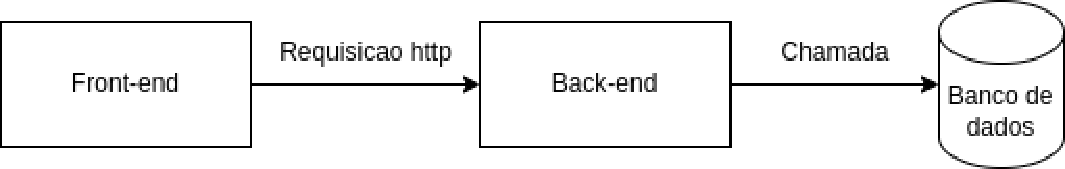
\includegraphics[width=0.75\textwidth]{figuras/arquitetura_antiga.pdf}
\caption{Estrutura geral antiga}
\label{estrutura_antiga}
\end{figure}

Considerando o modelo de arquitetura apresentado na Figura \ref{estrutura_antiga}, o procedimento para inserir um novo instituto exigia a replicação integral do código: front-end, back-end e a criação de um novo banco de dados independente. Isso resultava na criação separada de cada front-end, originando pequenas particularidades no desenvolvimento, embora os códigos fonte seguissem um modelo com considerável replicação entre os institutos. No back-end, a cada novo instituto, era necessário criar uma nova instância com código idêntico aos anteriores. O mesmo padrão era aplicado ao banco de dados, ou seja, uma nova instância era criada para cada instituto adicional.

Essa estrutura de código replicado ocasionou vários problemas. A manutenção do projeto tornou-se progressivamente mais complexa, trabalhosa e propensa a erros, uma vez que cada alteração demandava modificações em cada instância de código individualmente. Por exemplo, ao inserir um novo botão em todos os sites, era necessário modificar cada código fonte separadamente, resultando em desafios significativos na manutenção dos sites.

Com a arquitetura anterior, foram desenvolvidos sites para três institutos distintos: FAU, IME e FEARP, o que demandou o uso de três instâncias de máquinas virtuais na AWS. Essa abordagem resultou em um aumento de custos, uma vez que era necessário criar uma nova máquina virtual toda vez que um novo instituto era inserido no projeto. Embora, de acordo com a lógica de escalabilidade horizontal, isso fosse considerado uma qualidade do projeto, percebeu-se que a demanda pelo back-end era relativamente pequena. Portanto, concluiu-se que não seria necessário alocar uma máquina virtual exclusiva para a execução do back-end. A disposição das máquinas virtuais na AWS pode ser visualizada na figura a seguir.

\begin{figure}
    \centering
    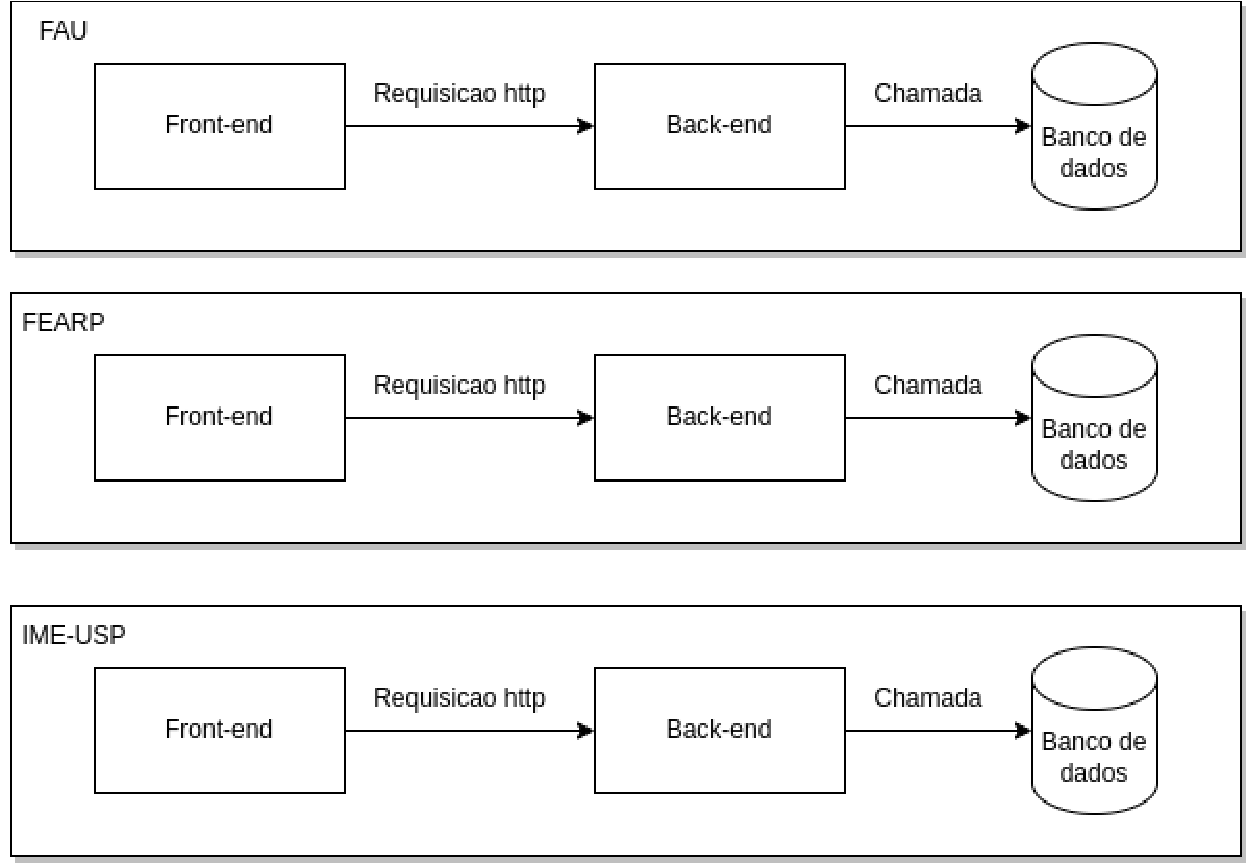
\includegraphics[width=0.75\linewidth]{figuras/arqtuitera_antiga_institutos.pdf}
    \caption{Estrutura antiga com os institutos que foram criados}
    \label{fig:arquitetura-antiga}
\end{figure}

Outra problemática presente na abordagem da arquitetura monolítica é a questão da segurança. A manutenção de todos os componentes agrupados em um único código base implica o compartilhamento do mesmo contexto de segurança. Em outras palavras, isso resulta em uma superfície de ataque maior, uma vez que uma vulnerabilidade em uma parte do sistema pode comprometer toda a plataforma.

Em resumo, a própria arquitetura se tornava um obstáculo para a escalabilidade do projeto, além de apresentar todas as dificuldades burocráticas relacionadas à obtenção de dados. Os custos associados à inclusão de novas unidades envolviam despesas financeiras (AWS), trabalho desnecessário por parte dos desenvolvedores e tempo a ser dedicado.


\section{Arquitetura Atual}

Visando corrigir esses problemas, buscou-se criar uma nova arquitetura que desacoplasse as diferentes partes do projeto. Inicialmente, separou-se o back-end e o front-end em diferentes repositórios para aprimorar a organização do projeto. A arquitetura Headless, que divide as responsabilidades entre o front-end, responsável pela interface de usuário, e o back-end, responsável pelo CMS e pela lógica de negócios, foi identificada como o sistema mais benéfico ao analisar os objetivos do projeto.

Anteriormente, cada instituto possuía um banco de dados próprio gerado dentro de um container Docker. Agora, esses bancos de dados individuais foram consolidados em uma única estrutura, utilizando uma tecnologia chamada RDS da Amazon, que armazena banco de dados PostgreSQL.

Essa nova estrutura de bancos de dados agregados possibilitou a unificação do back-end, uma vez que as requisições dos sites podiam ser filtradas, permitindo direcionar o back-end para o banco de dados apropriado em função dos diferentes tipos de consultas.

Os diferentes back-ends e bancos de dados criados para cada instituto foram unificados. Isso significa que os sites dos institutos poderiam requisitar dados de uma única API, resultando em apenas uma VM na AWS executando o back-end. Essa mudança não apenas reduziu os custos, mas também simplificou o processo de manutenção.

Uma nova camada para o CMS foi criada utilizando o Strapi, sendo responsável por gerir os estilos e estados dos diferentes sites. Nela, era possível armazenar os designs de cada site e modificá-los em tempo de execução. Em outras palavras, possibilitou a unificação do código-fonte do front-end, tornando viável a criação de páginas distintas utilizando a mesma estrutura. Essa nova arquitetura proporcionou facilidade na inserção de novos institutos, além de contribuir para a manutenção dos já existentes.

A figura a seguir (Figura \ref{fig:arquitetura-nova}) representa essa nova estrutura com os antigos institutos.

\begin{figure}
    \centering
    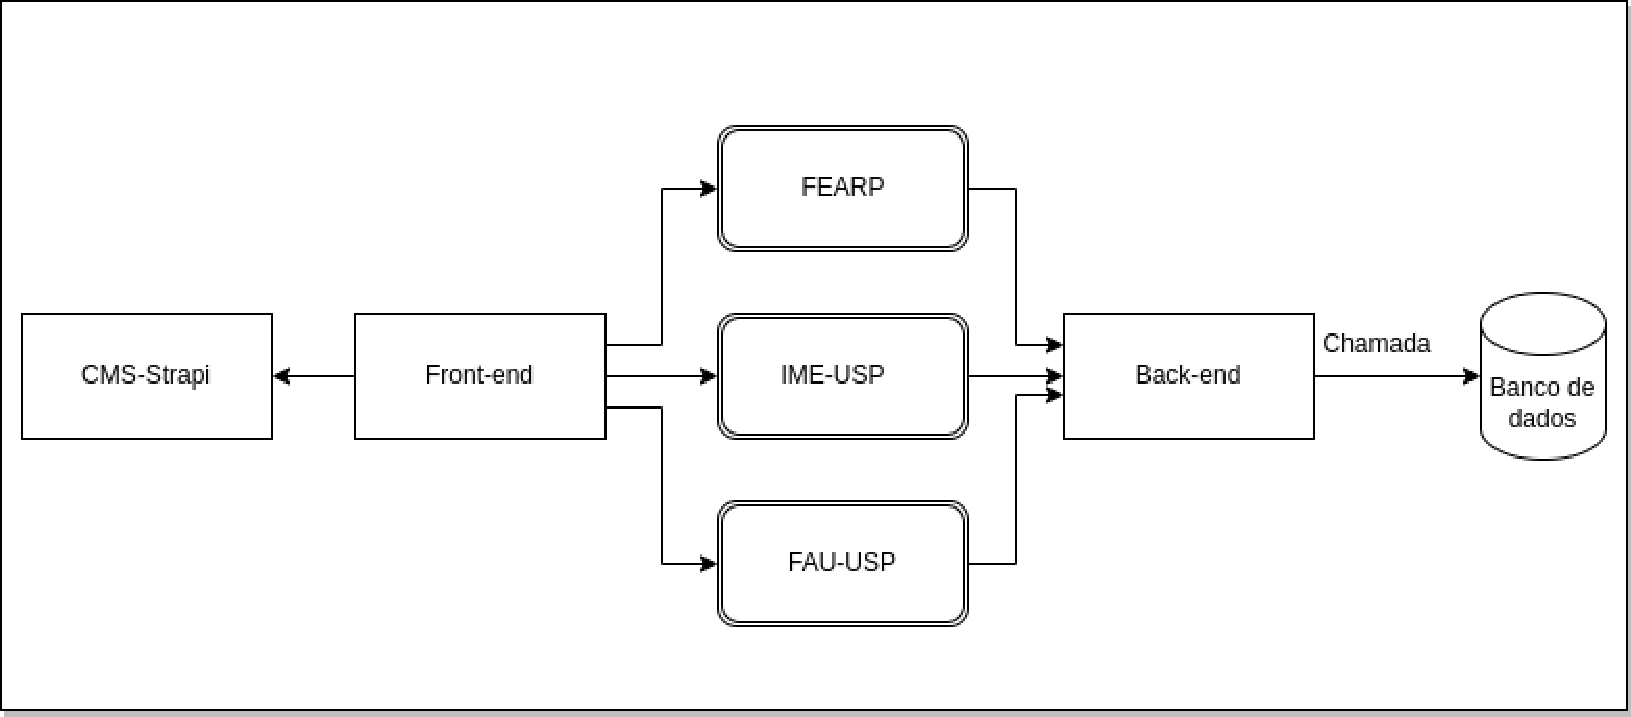
\includegraphics[width=0.75\linewidth]{figuras/nova_arquitetura.drawio-_1_.pdf}
    \caption{Estrutura novas com os institutos que foram criados}
    \label{fig:arquitetura-nova}
\end{figure}

Pela análise das imagens \ref{fig:arquitetura-antiga} e \ref{fig:arquitetura-nova}, é possível compreender melhor a questão da unificação. Na nova abordagem, há um front-end que realiza uma requisição para o CMS, gerando diferentes designs para os institutos. Quando o site é gerado, ocorre uma requisição para o back-end obter os dados referentes ao instituto em questão, direcionando a API para o banco de dados apropriado.

Atualmente, a instância do front-end utiliza o serviço da Amazon S3, que armazena arquivos e hospeda sites estáticos, como é o caso deste projeto que utiliza ReactJS. Para a hospedagem, basta utilizar a funcionalidade de build do framework, que gera um código HTML e, em seguida, é enviado para o serviço de armazenamento da Amazon. Dessa forma, não é mais necessário utilizar um container e uma VM para executar o front-end.

Portanto, na arquitetura atual, ocorre a build do código, que é o mesmo para todos os institutos, sendo a única diferença a especificação na variável ambiente indicando qual instituto está passando pelo processo.

\section{Opções e escolhas}
    \subsection{Headless CMS}
Um Headless CMS separa o conteúdo da apresentação, fornecendo esse conteúdo por meio de APIs para que os desenvolvedores possam escolher a forma de apresentação. Conceitualmente, o termo "headless" refere-se à separação da cabeça (front-end) do corpo (back-end), de forma semelhante ao Decoupled CMS. Embora ambos apresentem vantagens em aplicações complexas, o headless CMS se destaca ao enviar o conteúdo via API para diversos dispositivos, como dispositivos móveis e Internet das Coisas (IoT).

Ao comparar ambas as abordagens, decoupled e headless, a principal distinção está na flexibilidade de personalização. No atual projeto, em que a principal preocupação diz respeito à possível limitação na personalização, o headless CMS mostrou-se como a melhor alternativa.

Enquanto o decoupled CMS permite a desacoplagem do back-end e front-end, ainda mantendo opções de visualização pré-construídas, o headless CMS garante liberdade para criar interfaces de usuário (front-end) personalizadas para diferentes plataformas. Em outras palavras, a abordagem escolhida oferece total controle sobre a Interface de Usuário (UI), permitindo sua criação a partir do zero. Por outro lado, a outra alternativa proporciona maior flexibilidade em relação ao CMS tradicional, mas apresenta algumas opções pré-construídas.

Em contrapartida, existem algumas desvantagens na abordagem Headless. A escolha por maior flexibilidade de personalização implica maior dificuldade no uso, implementação, manutenção e gerenciamento. No entanto, a equipe responsável pela incorporação do Headless CMS realizou o estudo adequado e superou a curva de aprendizado apresentada.

    %%%%% grafico da curva

    \begin{figure}
        \centering
        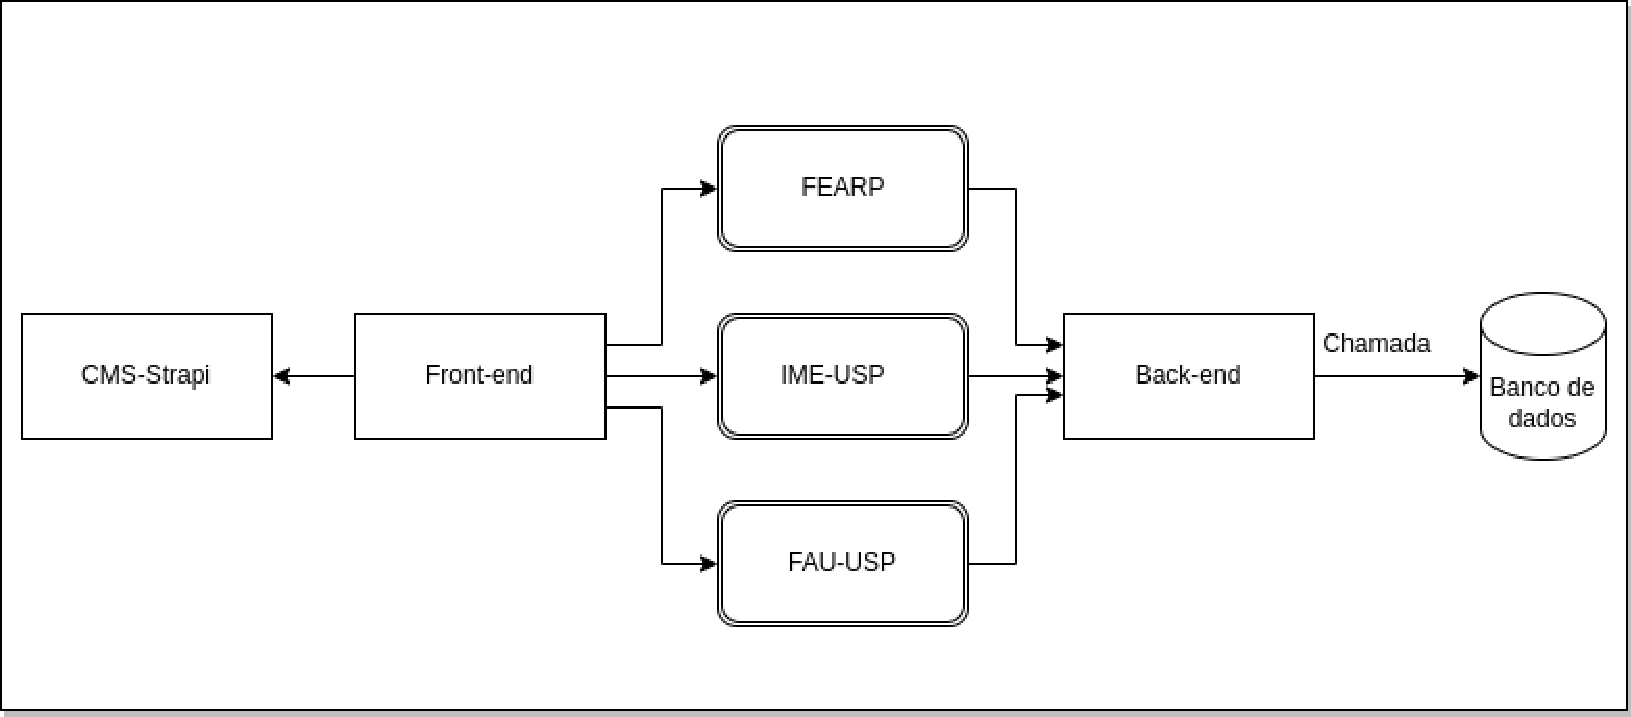
\includegraphics[width=0.75\linewidth]{figuras/nova_arquitetura.drawio-_1_.pdf}
        \caption{Gráfico de aprendizado para cada membro da equipe}
        \label{fig:learning-curve}
    \end{figure}

No gráfico \ref{fig:learning-curve}, foi retratada a porcentagem de domínio da nova tecnologia para cada membro da equipe de desenvolvedores. Observa-se que os membros que possuíam maior conhecimento em relação à linguagem do código herdado apresentaram maior facilidade para se adaptar à nova abordagem. Entretanto, membros cuja linguagem não era familiar no início do desenvolvimento enfrentaram maiores desafios ao lidar com a nova implementação.

Os dados para o gráfico foram coletados no período de 1 de agosto até o início de novembro, com intervalos aproximados de duas semanas entre cada coleta.

Outro fator determinante na escolha da abordagem Headless CMS foi a situação atual das empresas no mercado de trabalho. No início do projeto, foi realizada uma reunião com desenvolvedores de plataformas web de algumas empresas, onde o Strapi foi indicado como a melhor ferramenta para incorporar o sistema headless no projeto.

    Em conclusão, a adoção de um Headless CMS, que separa o conteúdo da apresentação, revelou-se uma escolha estratégica para o atual projeto. Conceitualmente, a abordagem "headless" transcende a metáfora de separar a cabeça (front-end) do corpo (back-end), oferecendo uma vantagem crucial ao enviar o conteúdo através de APIs para diversos dispositivos, como dispositivos móveis e Internet das Coisas (IoT). A comparação entre as abordagens decoupled e headless destacou a principal distinção na flexibilidade de personalização, sendo que o Headless CMS proporcionou a liberdade desejada para criar interfaces de usuário personalizadas para diferentes plataformas. Embora esta escolha tenha apresentado desafios em termos de dificuldade de uso, implementação, manutenção e gerenciamento, a equipe dedicada superou eficazmente a curva de aprendizado, conforme evidenciado no gráfico de aprendizado apresentado. A análise do domínio tecnológico revelou que membros da equipe com conhecimento prévio na linguagem de código herdado tiveram uma transição mais suave para a nova abordagem. Além disso, a consulta inicial a especialistas do mercado de trabalho, que recomendaram o Strapi como a melhor ferramenta para incorporar um sistema headless, solidificou a decisão estratégica. Assim, a escolha do Headless CMS foi respaldada por sua capacidade única de oferecer personalização sem restrições, essencial para atender às demandas específicas do projeto em questão.

    \subsection{Tecnologia Strapi}

   Em relação à escolha tecnológica, as principais alternativas consideradas além do Strapi incluíram o Contentful, o GraphCMS e o Sanity, plataformas de CMS headless amplamente reconhecidas. A decisão de optar pelo Strapi foi fundamentada na aderência à filosofia do Software Livre, destacando-se como um diferencial a sua natureza de código aberto. Este atributo se traduz em uma vantagem significativa, especialmente no que se refere ao extenso ecossistema de plugins. A abertura do código amplia o conjunto de desenvolvedores capacitados a criar plugins, resultando em uma maior diversidade e quantidade de extensões disponíveis.

    É válido mencionar que, embora a escolha pelo Strapi tenha apresentado inúmeras vantagens, algumas desvantagens foram identificadas, embora consideradas menos impactantes pela equipe. Por exemplo, plataformas como o GraphCMS e o Sanity oferecem recursos que aprimoram a colaboração em equipe, como controle de versão e atribuição de tarefas diretamente na plataforma. No entanto, ao explorar o catálogo de plugins do Strapi, foram identificados plugins direcionados ao controle de versão (Content Versioning), enquanto a edição colaborativa poderia ser abordada por meio de um recurso específico, o Strapi Cloud, disponível apenas para usuários pagos.

    Outra consideração abordada refere-se à manipulação de imagens e assets dinâmicos. Embora plataformas como Contentful e Sanity ofereçam abordagens diferenciadas para a manipulação desses dados, no atual contexto do projeto, a presença limitada de imagens, essencialmente relacionadas aos logotipos institucionais, minimizou a relevância desses recursos específicos.

    Em síntese, a escolha do Strapi como plataforma para o desenvolvimento do sistema revelou-se alinhada aos princípios fundamentais do projeto, notadamente no que concerne à adesão à filosofia do Software Livre. A natureza de código aberto do Strapi proporcionou não apenas uma flexibilidade ímpar, mas também um robusto ecossistema de plugins, garantindo uma personalização eficaz e a disponibilidade de uma ampla gama de recursos adicionais. Embora a análise criteriosa tenha evidenciado algumas desvantagens, como a necessidade de recursos pagos para funcionalidades específicas e a abordagem diferenciada de plataformas concorrentes em aspectos colaborativos, esses aspectos foram considerados secundários diante da solidez e adaptabilidade que o Strapi ofereceu ao projeto. A decisão fundamentada na busca pelo equilíbrio entre recursos, filosofia, e necessidades específicas, culminou em uma escolha que não apenas atendeu, mas também enriqueceu os objetivos propostos.
\chapter{Funcionamento e tecnologias}
\label{chap:funcionamento}

\enlargethispage{-.5\baselineskip}

\section{Processo de desenvolvimento}
   Durante o período de desenvolvimento, a equipe adotou a Metodologia Ágil. Dada a complexidade do processo de desenvolvimento de software, a utilização de um modelo único mostrou-se insuficiente e ineficaz. A abordagem ágil foi escolhida devido aos benefícios de sua natureza adaptativa e personalizada, proporcionando não apenas desenvolvimento mais rápido e eficaz, mas também maturidade à organização, conforme discutido por \cite{8229928}.

    Nesse contexto, os principais marcos temporais do ciclo de desenvolvimento foram estabelecidos como Milestones. Em resumo, esses marcos representam metas específicas a serem alcançadas em momentos determinados, auxiliando na divisão do processo em fases gerenciáveis. Isso permite o acompanhamento do progresso e a avaliação do cumprimento de objetivos em momentos-chave.

   \begin{figure}[!htb]
       \centering
       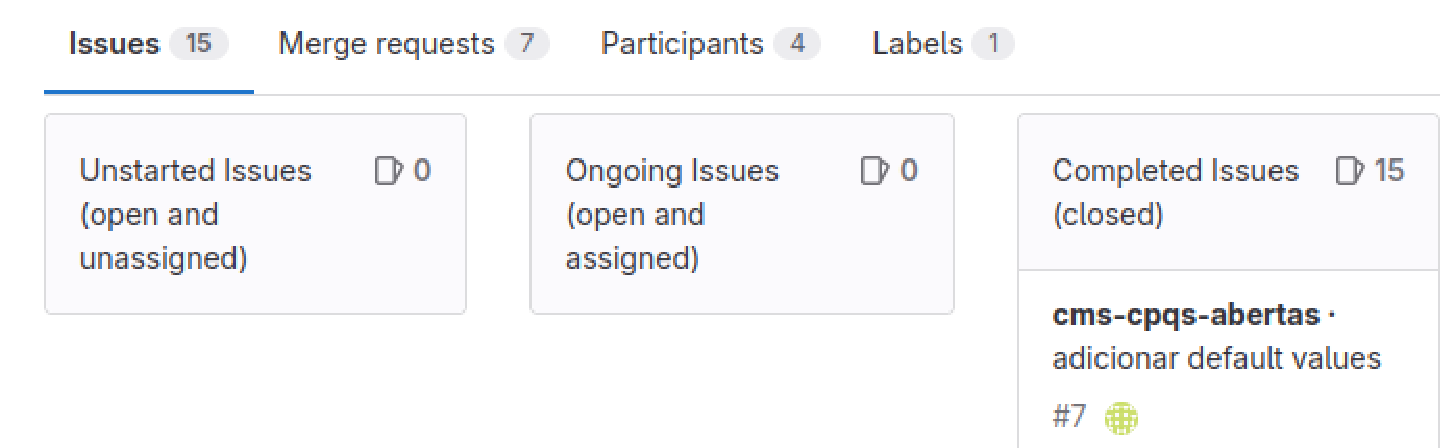
\includegraphics[width=0.75\textwidth]{figuras/milestones.pdf}
       \caption{Milestone: visualização Scrum Board}
       \label{milestones}
    \end{figure}

 Além disso, dentro de cada Milestone, a administração era conduzida por meio da visualização em forma de Scrum Board, conforme ilustrado em \ref{milestones}. Essa ferramenta visual geralmente consiste em colunas representando etapas como "To Do", "In Progress" e "Done". Dessa forma, foi possível obter uma visão rápida do status de cada issue ou tarefa.

As issues ou tarefas, por sua vez, podem se referir a bugs, melhorias ou qualquer unidade de trabalho identificada e registrada no sistema de controle e gerenciamento. É importante ressaltar que não havia um formato padrão de issue: algumas eram abrangentes e continham subitens para auxiliar no entendimento, enquanto outras eram curtas e gerais.

Para cada issue realizada, o código referente à melhoria era adicionado a uma branch, ou seja, a uma versão independente do código-fonte no repositório do Gitlab. Esse uso permitiu que todos os desenvolvedores da equipe trabalhassem em recursos separados sem interferir uns nos outros.

Ao concluir a issue, era efetuado um Pull Request, ou seja, uma solicitação para incorporar as alterações de uma branch ao código principal. A aprovação dessas requisições ocorria após a realização do code review, prática essencial em metodologias ágeis. Esse método envolve a revisão sistemática e colaborativa do código por outros membros da equipe. Durante cada revisão, o membro responsável garantia que o código estivesse em conformidade com os padrões de codificação, diretrizes e práticas estabelecidas pela equipe.

\section{Strapi}
Como mencionado em seções anteriores, a estratégia adotada para avançar no desenvolvimento do projeto foi a utilização do Headless CMS, com destaque para a abordagem empregada pelo Strapi. O Strapi é uma ferramenta de gerenciamento de conteúdo de código aberto que utiliza Node.js. Seu papel central inclui a disponibilização de APIs e a organização dos conteúdos de maneira clara e intuitiva.

Na atual paisagem de desenvolvimento web, a gestão de conteúdo digital desempenha um papel fundamental na construção de sites e aplicativos interativos e dinâmicos. O Strapi destaca-se como uma solução notável e inovadora nesse cenário, oferecendo um sistema de gerenciamento de conteúdo de código aberto que se diferencia por sua flexibilidade, personalização e capacidade de criar e gerenciar APIs robustas. Projetado para atender às necessidades dos desenvolvedores modernos que buscam uma abordagem mais flexível na gestão de conteúdo, o Strapi permite que os desenvolvedores criem, modifiquem e organizem facilmente o conteúdo digital conforme as especificações de seus projetos. Essa flexibilidade é alcançada por meio de uma arquitetura de plugin extensível, que facilita a adição de funcionalidades personalizadas de maneira simples e eficaz.

Uma das características mais distintivas do Strapi é sua habilidade de gerar automaticamente APIs RESTful e GraphQL com base no conteúdo definido no sistema. Isso implica não apenas a capacidade de criar conteúdo, mas também de expô-lo facilmente para uso em aplicativos web, móveis e outros sistemas. A capacidade de oferecer acesso a dados estruturados por meio de APIs é especialmente valiosa em um mundo digital altamente interconectado. O Strapi foi concebido com interoperabilidade em mente, suportando vários tipos de bancos de dados. Essa abertura possibilita aos desenvolvedores escolher o sistema de armazenamento de dados que melhor se alinha às necessidades de seus projetos, desde bancos de dados SQL tradicionais até soluções NoSQL. Essa flexibilidade é essencial para integrar o Strapi em diversos contextos de desenvolvimento.

Outra vantagem significativa da ferramenta é sua interface de usuário intuitiva e amigável. Isso simplifica a criação e gestão de conteúdo, tornando o Strapi acessível mesmo a usuários não técnicos. No entanto, a plataforma também oferece uma estrutura orientada para desenvolvedores que possibilita personalizações avançadas. Isso garante que as equipes de desenvolvimento possam criar experiências de usuário refinadas e complexas, ao mesmo tempo em que os editores de conteúdo consigam gerenciar o conteúdo de forma fácil, sem depender constantemente de intervenção técnica.

O núcleo do Headless CMS, presente no gerenciador de conteúdo da ferramenta, é onde reside a essência do Strapi. Nele, são listados os chamados 'Collection Types', cuja definição depende do contexto específico do projeto. No caso do CpqsAbertas, por exemplo, temos Institutos e Departamentos como coleções distintas. Nesse contexto, Departamentos representam unidades específicas, como MAT, DCC, MAE, etc., enquanto Institutos servem como representação das faculdades em si, como IME, FAU, FEARP. Cada 'Collection Type' possui campos variados, como texto, JSON, números, relações, entre outros. O preenchimento desses campos é crucial, pois é por meio deles que a API é alimentada.

%%%%%%%%%%%%%%%%%%%%%%%%%%%%%%%%%%%%
%(talvez inserir aqui um print da página do strapi que lista os campos disponíveis para uso)

%%%%%%%%%%%%%%%%%%%%%%%%%%%%5
O Strapi ganhou popularidade em diversos cenários de desenvolvimento web e de aplicativos, sendo frequentemente escolhido para projetos que demandam um alto grau de controle sobre o conteúdo e sua exposição por meio de APIs. Essa escolha abrange uma ampla gama de casos de uso, desde sites corporativos e blogs até aplicativos móveis, lojas online e sistemas de gerenciamento de conteúdo complexos. Essa versatilidade demonstra a adaptabilidade e a eficácia do Strapi em atender às necessidades de diferentes tipos de projetos.

Ao adotar o modelo de arquitetura Headless CMS, por meio da implementação eficaz do Strapi, o Projeto Cpqs-abertas experimentou uma transformação significativa em sua infraestrutura e metodologia de desenvolvimento. A transição de uma abordagem monolítica para uma estrutura mais flexível e desacoplada proporcionou não apenas uma gestão mais eficiente do conteúdo, mas também uma maior adaptabilidade às demandas em constante evolução do projeto. A estratégia "white label" e o uso estratégico de um Sistema de Gerenciamento de Conteúdo (CMS) desempenharam papéis fundamentais na unificação e manutenção contínua do projeto, permitindo que ele cumprisse sua missão de disseminar conhecimento de forma eficaz e colaborativa. A escolha do Strapi, com sua capacidade de gerar APIs automaticamente e oferecer flexibilidade na gestão de conteúdo, destacou-se como um elemento central para alcançar o equilíbrio entre personalização avançada e simplicidade na administração do sistema. Essa seção revela não apenas uma evolução tecnológica, mas também um alinhamento estratégico crucial para o Cpqs-abertas, marcando um capítulo significativo em sua trajetória de desenvolvimento.

\section{Manutenção AWS}

\section{Disseminação Software Livre}
Uma das motivações intrínsecas do projeto, desde a sua concepção, está vinculada à sua participação ativa na comunidade de Software Livre. Seguindo a definição da Free Software Foundation, uma embaixadora desse movimento, o Software Livre proporciona o controle sobre a tecnologia utilizada em nossas residências, escolas e negócios. Este controle visa o benefício individual e coletivo, não sendo submetido a empresas de software proprietário ou governos que buscam restringir e monitorar os usuários.
    
    \begin{quote}
     \enquote{Free software is about having control over the technology we use in our homes, schools and businesses, where computers work for our individual and communal benefit, not for proprietary software companies or governments who might seek to restrict and monitor us.}
    \end{quote}

Nesse contexto, a base essencial para o sucesso de um software na comunidade de Software Livre é sua hospedagem em plataformas de código aberto. Atualmente, as opções mais populares incluem o GitHub, GitLab e Bitbucket. Durante a fundação do projeto CPQs Abertas, esse critério teve influência decisiva na escolha, e o projeto está hospedado no GitLab. Além disso, a escolha da licença é de extrema importância, levando à escolha da MIT, cujas principais características incluem permissividade, reutilização livre e liberdade de uso. Essa licença também é compatível com outras, permitindo sua combinação no mesmo software, inclusive com software proprietário. É vital, no entanto, manter a nota de direitos autorais e a isenção de responsabilidade em todas as cópias do software.

Durante o desenvolvimento, é crucial manter uma documentação abrangente e fornecer um canal de comunicação aberto. No caso do CPQs Abertas, após cada período de trabalho dos grupos, a documentação era obrigatoriamente atualizada para incluir explicações detalhadas sobre instalação, configuração e uso do software. Isso facilitaria a contribuição de novos desenvolvedores para o projeto. No que diz respeito ao canal de comunicação, as issues relacionadas a determinado período eram atualizadas conforme sua execução. Adicionalmente, foi organizado um procedimento para adicionar e documentar cada uma das issues pendentes ao final do período de desenvolvimento, visando facilitar para os próximos desenvolvedores.

Apesar da base existente, o projeto ainda não alcançou o reconhecimento necessário na comunidade de Software Livre, limitando-se ao desenvolvimento por grupos anuais de alunos. Isso destaca a importância de construir uma comunidade mais ampla e promover a disseminação do projeto. Dado o desejo dos fundadores de transformar o projeto em um verdadeiro software de código aberto com contribuições ativas, é imperativo trabalhar nesse aspecto. Para os futuros desenvolvedores da CPQs Abertas, especialmente se não houver a necessidade imediata de lidar com mudanças estruturais, é desejável dedicar esforços nesse sentido. Isso pode ser realizado por meio de palestras, apresentações, participação em conferências relacionadas ao código aberto e divulgação online.

Nesta etapa, para conquistar espaço e visibilidade em mídias de grande alcance, é essencial contar com o apoio de influentes dentro da Universidade, além de obter reconhecimento de todas as unidades da USP. O principal desafio estava relacionado à dificuldade de criar e manter atualizadas novas plataformas web. Administrar várias plataformas simultaneamente sem recursos adequados é inviável. Os recursos implementados pela equipe solucionam questões emergenciais relacionadas à escalabilidade, possibilitando a construção quase imediata de plataformas web para cada unidade. A única barreira é a obtenção dos dados do Lattes, uma vez que a equipe da CPqs Abertas não tem acesso direto a essas informações.

A estratégia de implementação baseada em White Label tem como principal objetivo reduzir os custos de produção, permitindo um foco maior no marketing e divulgação. Com as melhorias implementadas, é razoável afirmar que, a médio prazo, haverá um reconhecimento suficiente por parte da comunidade acadêmica e universitária. Isso abrirá caminho para buscar apoio em mídias de divulgação mais amplas.

Em síntese, a orientação do projeto CPQs Abertas em direção à filosofia do Software Livre, embasada nos princípios de controle tecnológico descentralizado e benefício coletivo, reflete-se na escolha estratégica de plataformas de código aberto, como o GitLab, e na adoção da licença MIT. Estes fundamentos não apenas alinham o projeto com os valores essenciais do movimento, mas também estabelecem uma base sólida para o engajamento e contribuições da comunidade. No entanto, o desafio persiste na ampliação do reconhecimento e participação, sendo essencial explorar estratégias de divulgação em eventos, palestras e meios online. A busca pelo apoio de detentores de poder na Universidade, bem como o aprimoramento constante da infraestrutura técnica, são passos fundamentais para superar as barreiras que limitam o crescimento do projeto. Ao promover uma cultura de Software Livre e fortalecer a comunidade ao seu redor, o CPQs Abertas pode solidificar sua posição como uma contribuição valiosa para a disseminação do conhecimento acadêmico em um contexto aberto e colaborativo.
\chapter{Implementação}
\label{chap:implementacao}
\section{section}
\chapter{Conclusão}
\label{chap:conclusao}


%%%% Apêndices %%%%

\makeatletter
\if@openright\cleardoublepage\else\clearpage\fi
\makeatother


%%%%%%%%%%%%%%% SEÇÕES FINAIS (BIBLIOGRAFIA E ÍNDICE REMISSIVO) %%%%%%%%%%%%%%%%

% O comando backmatter desabilita a numeração de capítulos.
\backmatter

%\pagestyle{backmatter}

% Espaço adicional no sumário antes das referências / índice remissivo
\addtocontents{toc}{\vspace{2\baselineskip plus .5\baselineskip minus .5\baselineskip}}

% A bibliografia é obrigatória

\printbibliography[
  title=\refname\label{bibliografia}, % "Rseferências", recomendado pela ABNT
  %title=\bibname\label{bibliografia}, % "Bibliografia"
  heading=bibintoc, % Inclui a bibliografia no sumário
]

\printindex % imprime o índice remissivo no documento (opcional)

\end{document}
